% !TEX root = ../projekt.tex
% =============================================================================
% STAV: všetky doplnkové grafy z porovnania hashov (staršia verzia kódu, thesis_results/).
% =============================================================================
\chapter{Doplnkové grafy porovnania hashovacích funkcií}
\label{app:grafy}

Príloha obsahuje grafy ďalších vzoriek prevádzky. Pochádzajú zo staršej verzie simulátora: používajú 128 položiek RETA, 16 kľúčov, pevné okno 150\,000 paketov a namiesto jednoduchej tabelácie funkciu multiply-shift (NH). Grafy pre \texttt{odid1} s~plným tuple a aktuálnou sadou funkcií sú v~kapitole~\ref{chap:analyza}.

\TODO{Prekresliť so slovenskými popismi po prepočítaní novým simulátorom.}

\clearpage
\begin{figure}[p]
  \centering
  \begin{subfigure}{0.60\textwidth}
    \centering
    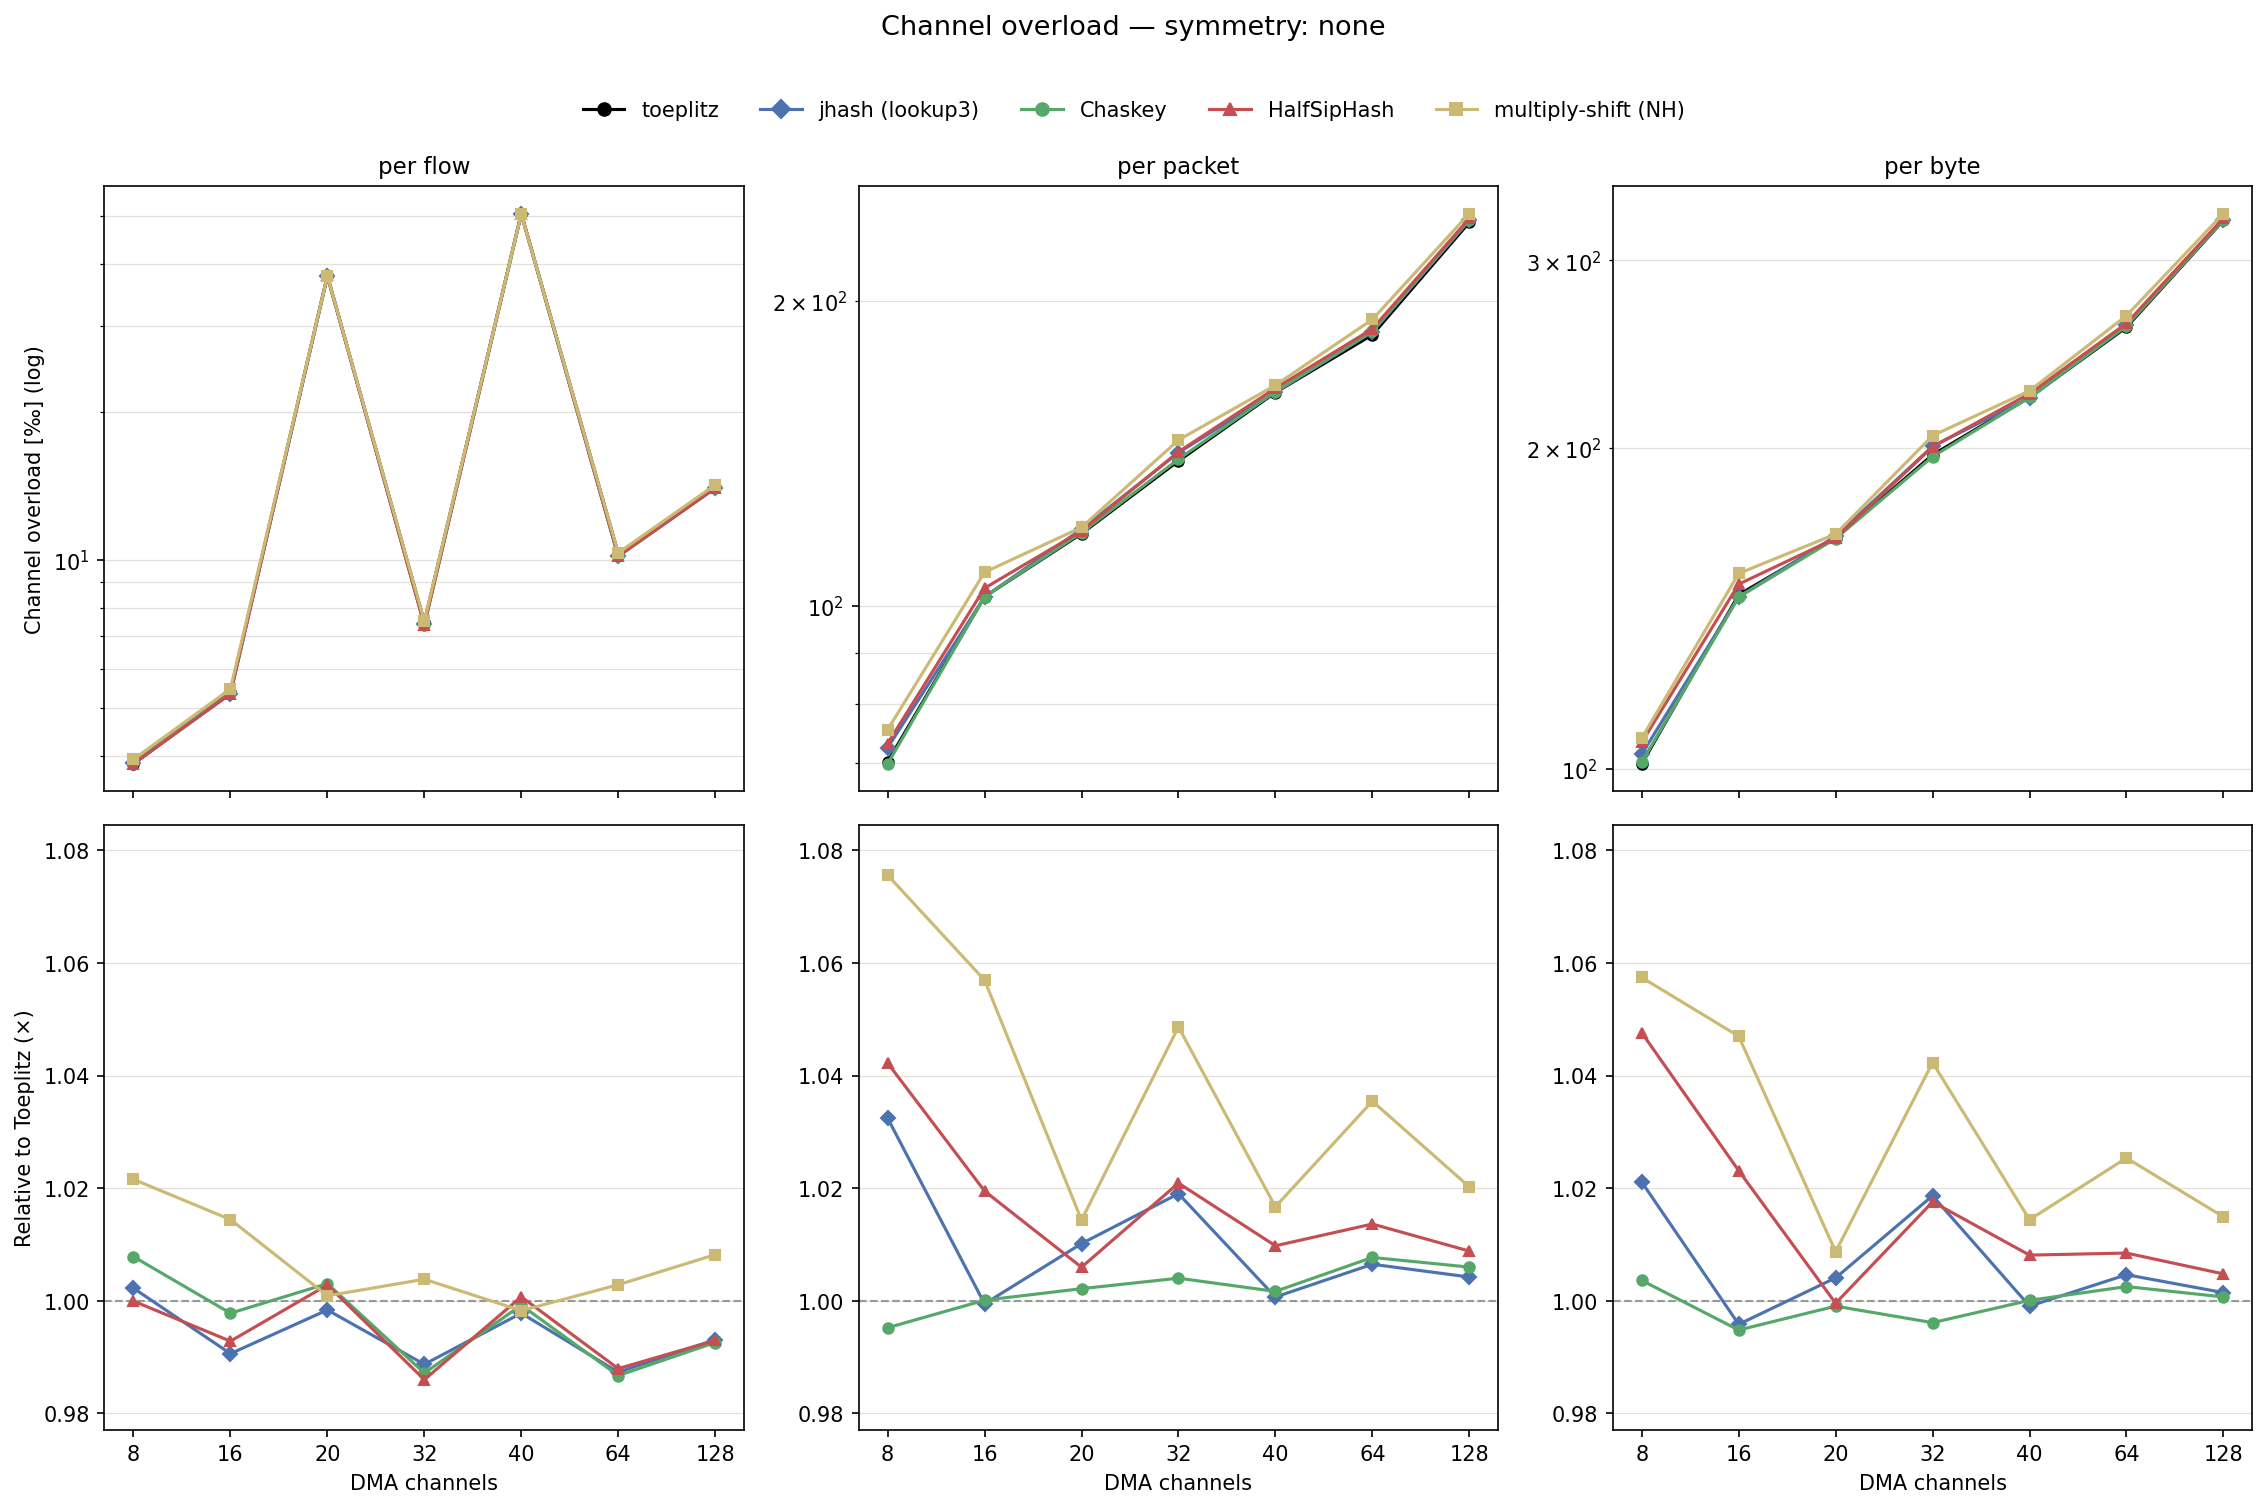
\includegraphics[width=\textwidth]{ostatne_vzorky/odid2_full_tuple/overload_none.png}
    \caption{bez symetrie}
  \end{subfigure}

  \begin{subfigure}{0.60\textwidth}
    \centering
    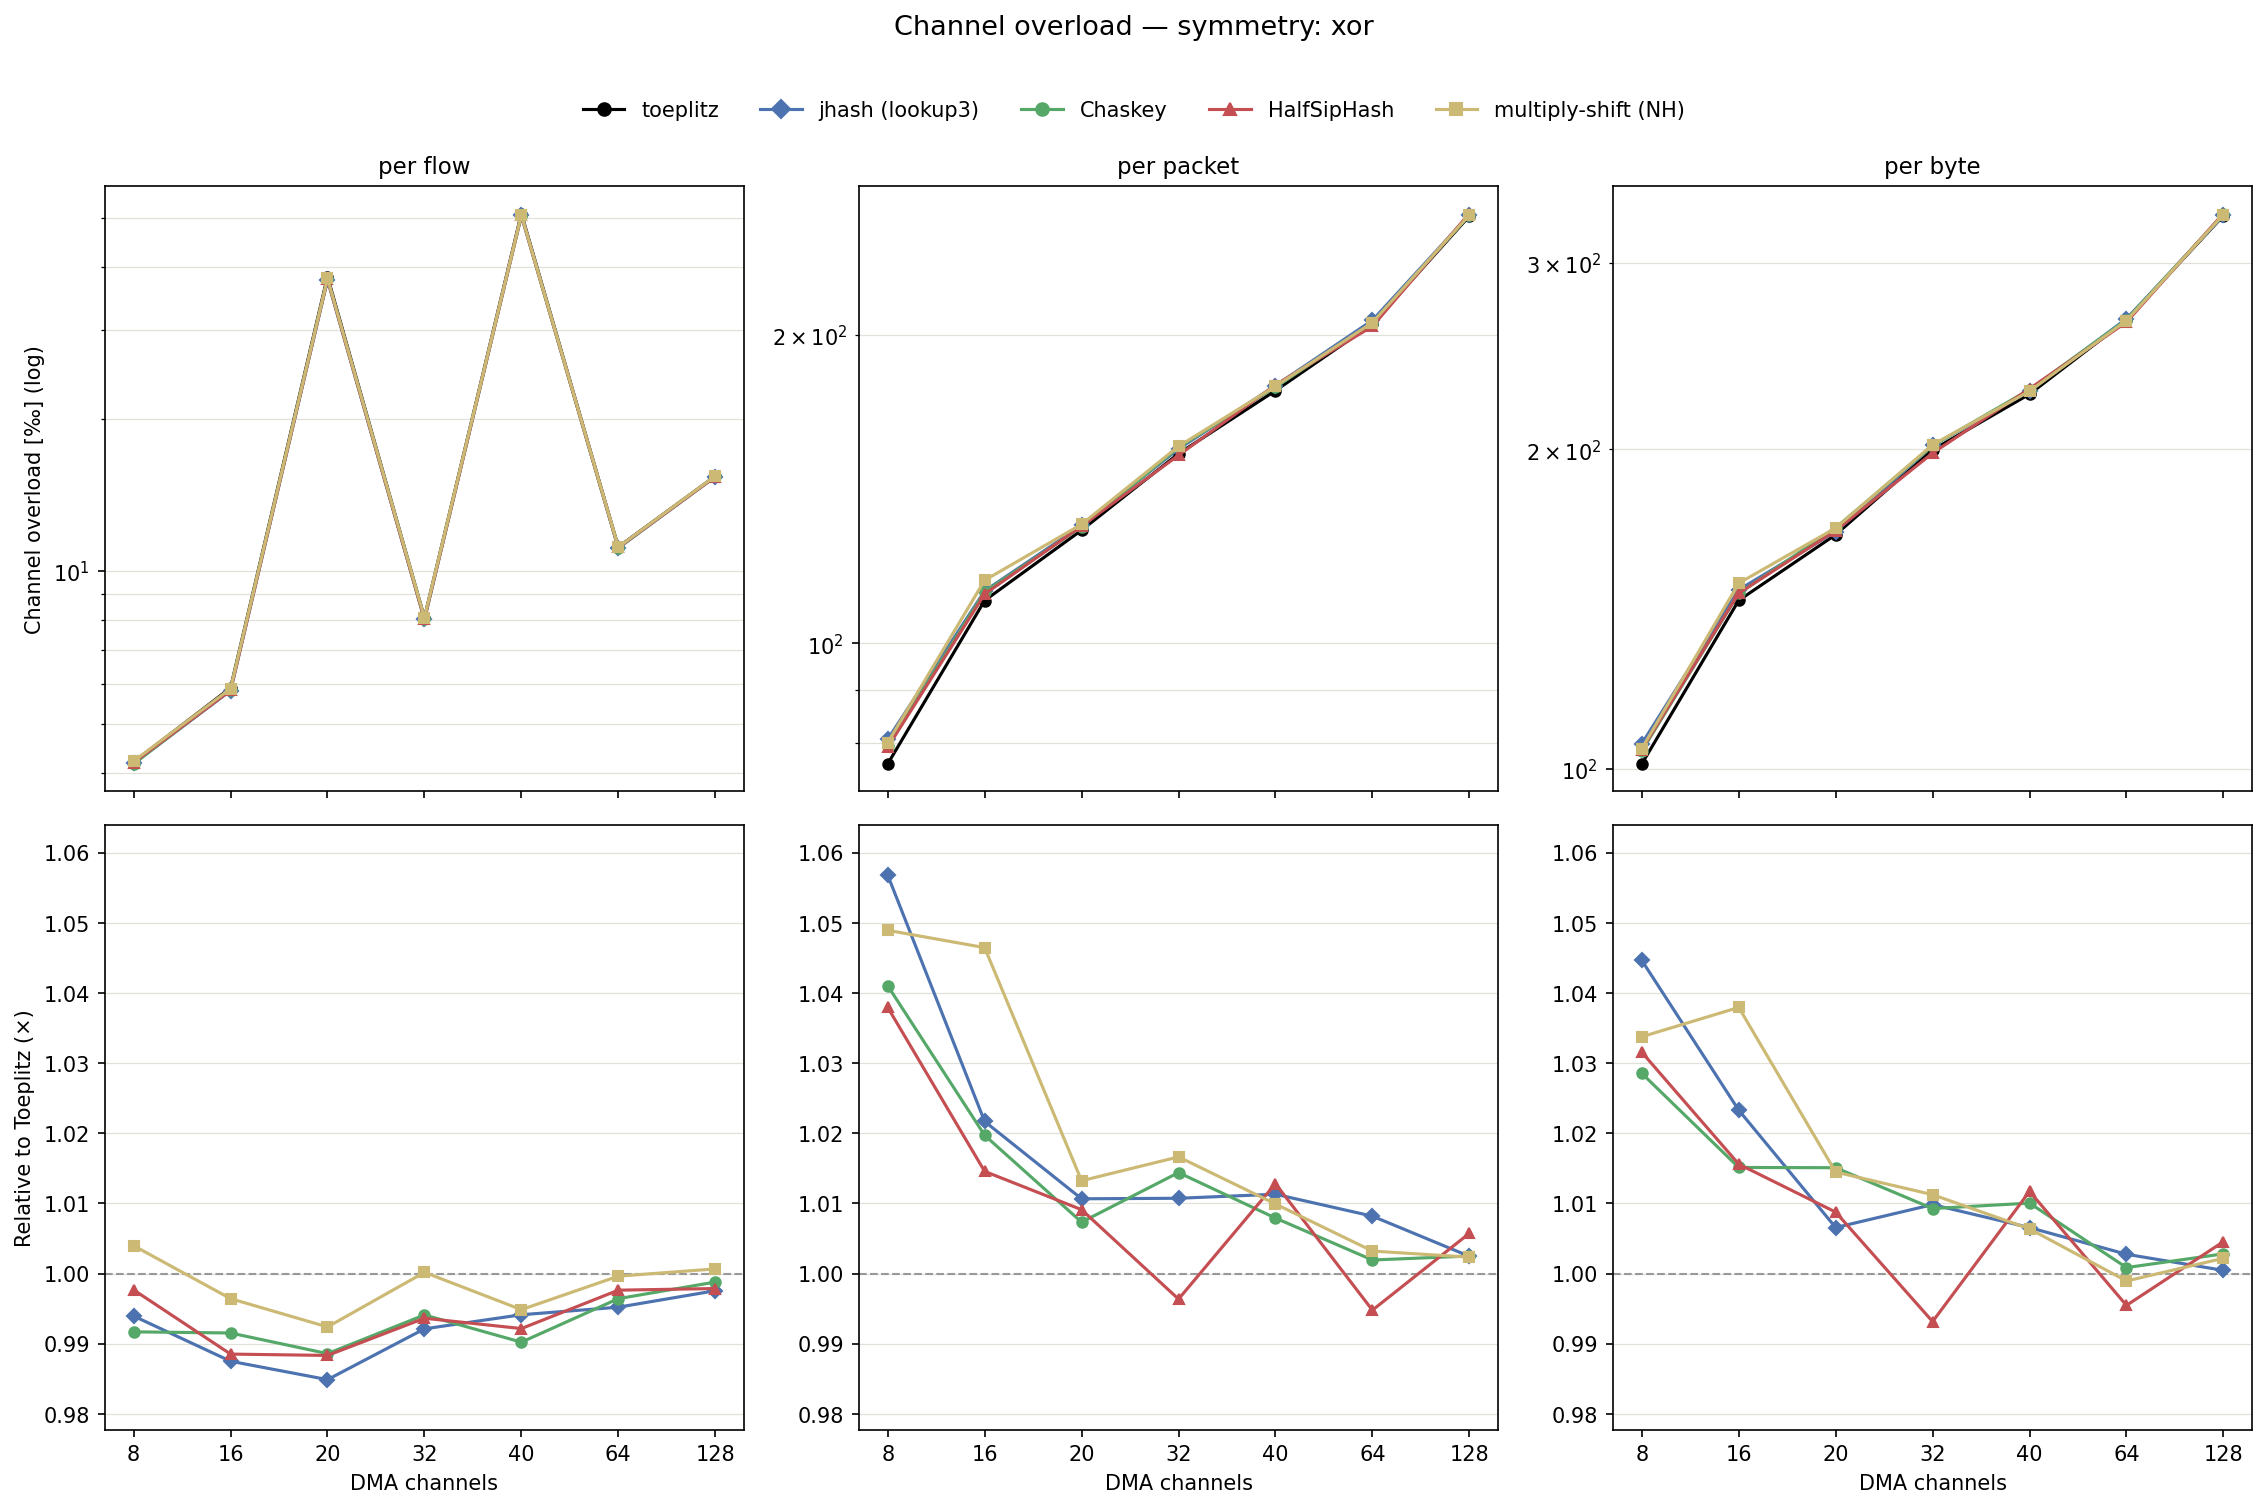
\includegraphics[width=\textwidth]{ostatne_vzorky/odid2_full_tuple/overload_xorfold.png}
    \caption{symetria XOR}
  \end{subfigure}

  \begin{subfigure}{0.60\textwidth}
    \centering
    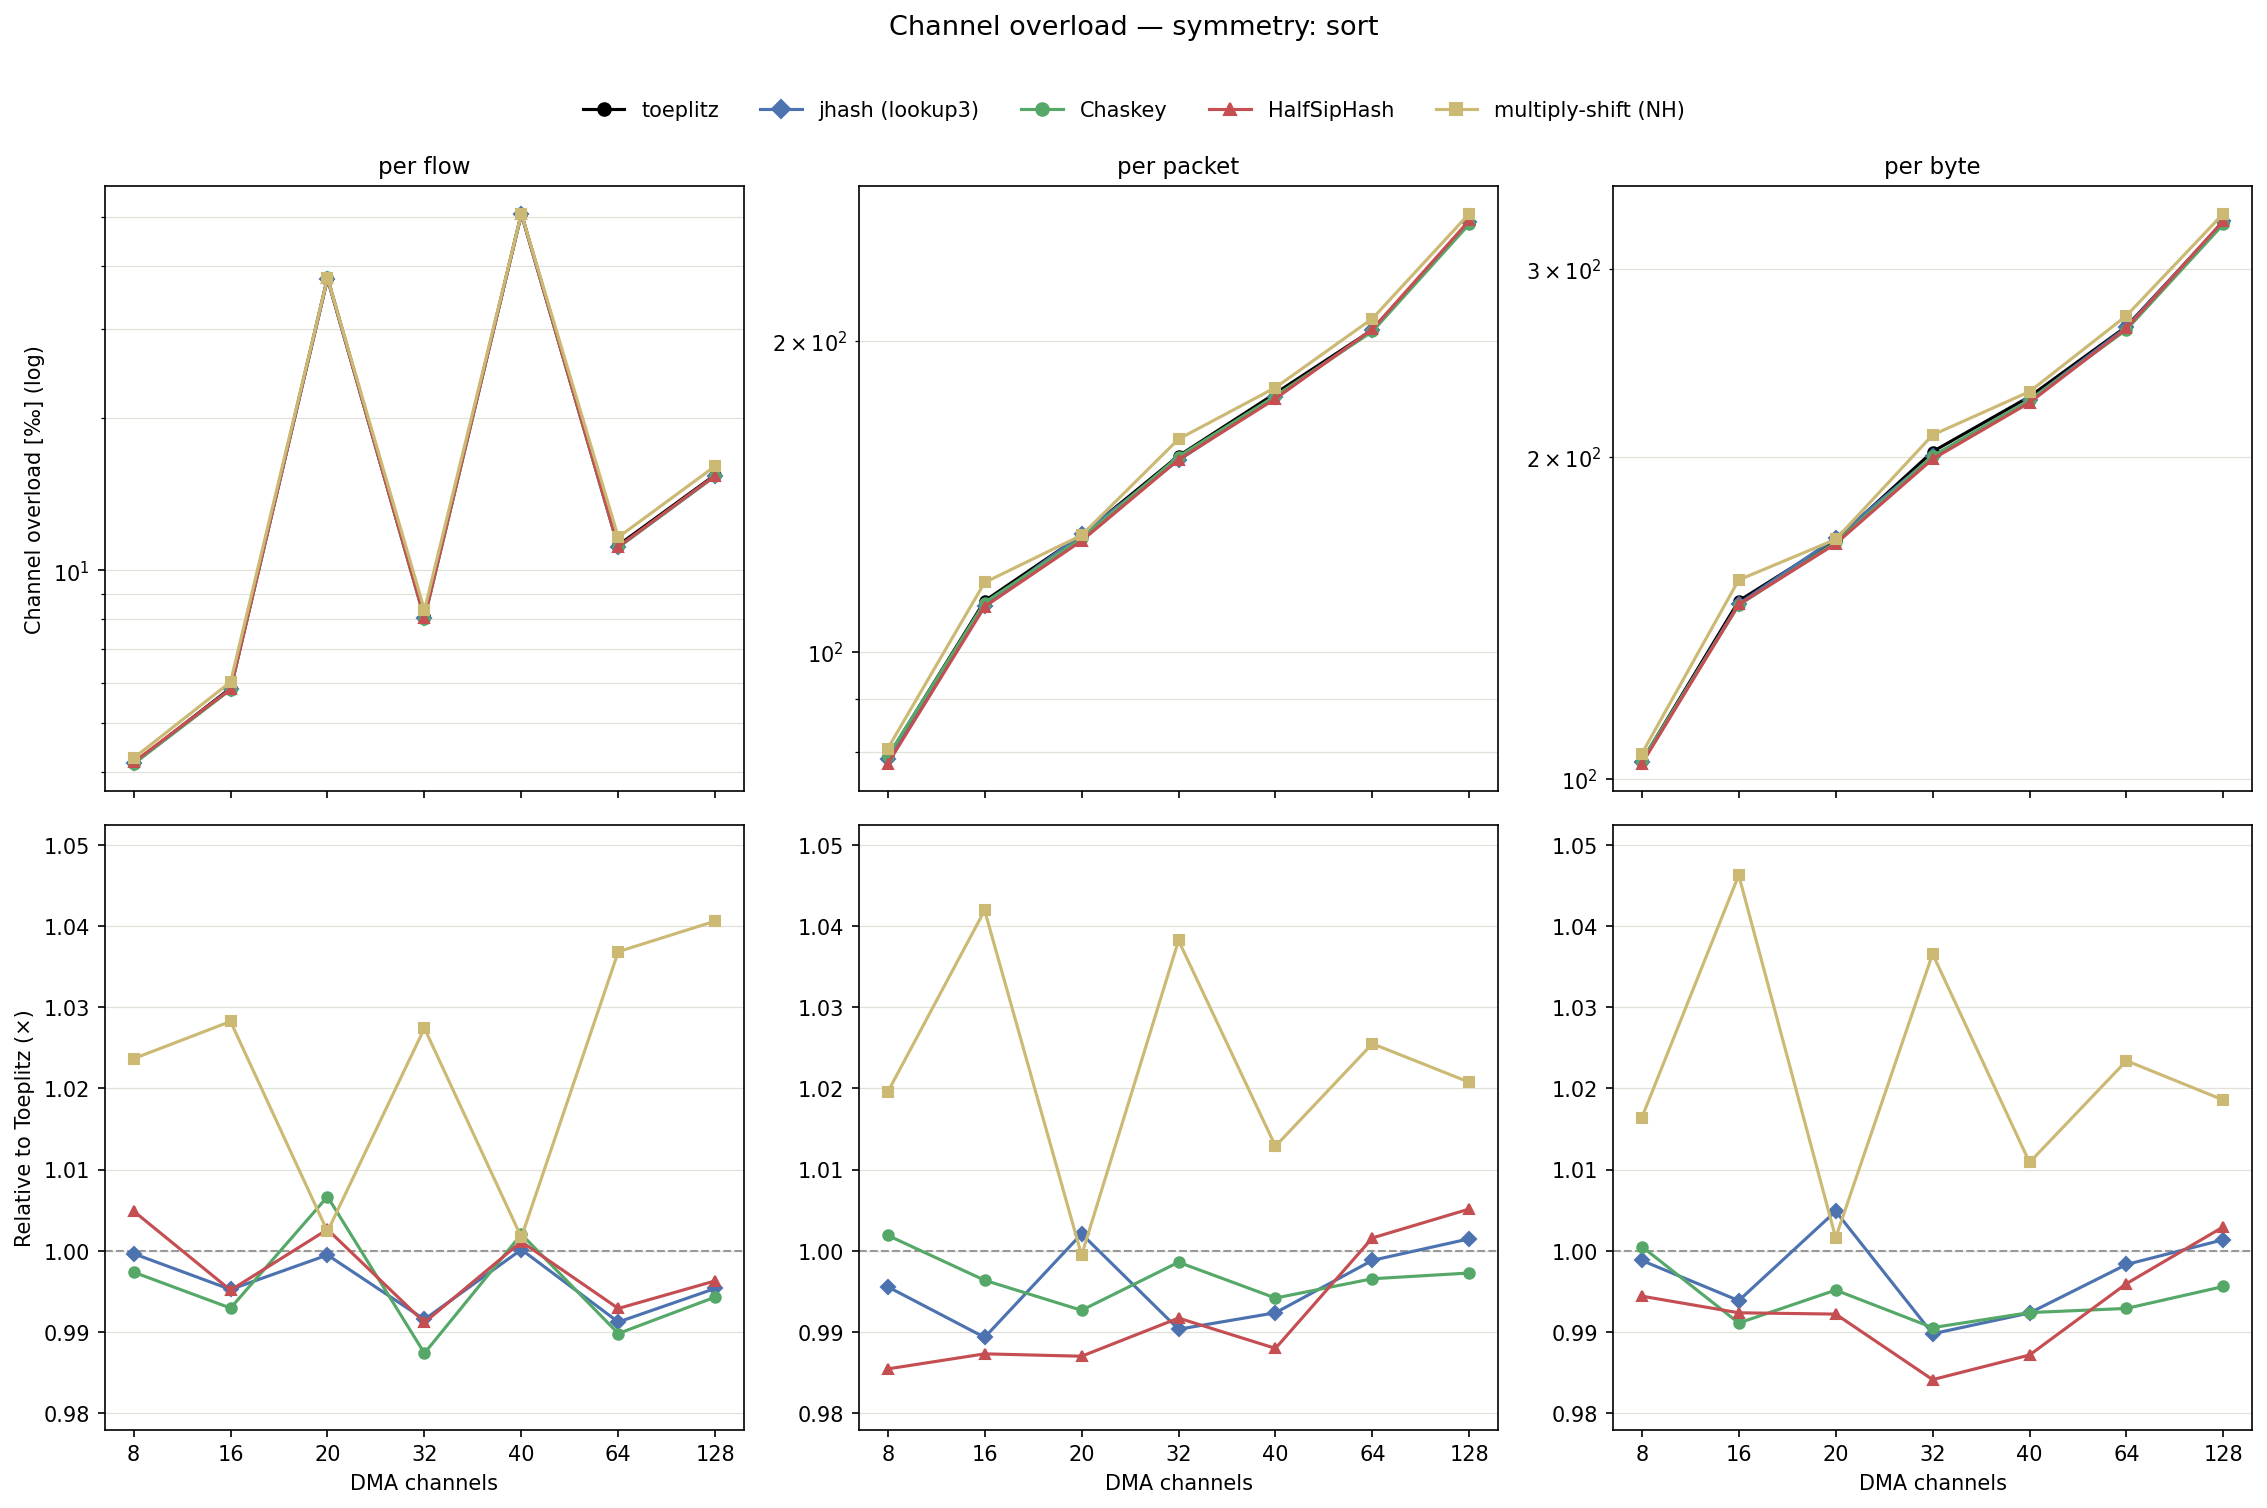
\includegraphics[width=\textwidth]{ostatne_vzorky/odid2_full_tuple/overload_sortfold.png}
    \caption{symetria sort}
  \end{subfigure}

  \caption{Preťaženie funkcií a pomer k~Toeplitzu: \texttt{odid2}, plný tuple.}
  \label{fig:b-odid2-full-tuple-overload}
\end{figure}

\begin{figure}[p]
  \centering
  \begin{subfigure}{0.54\textwidth}
    \centering
    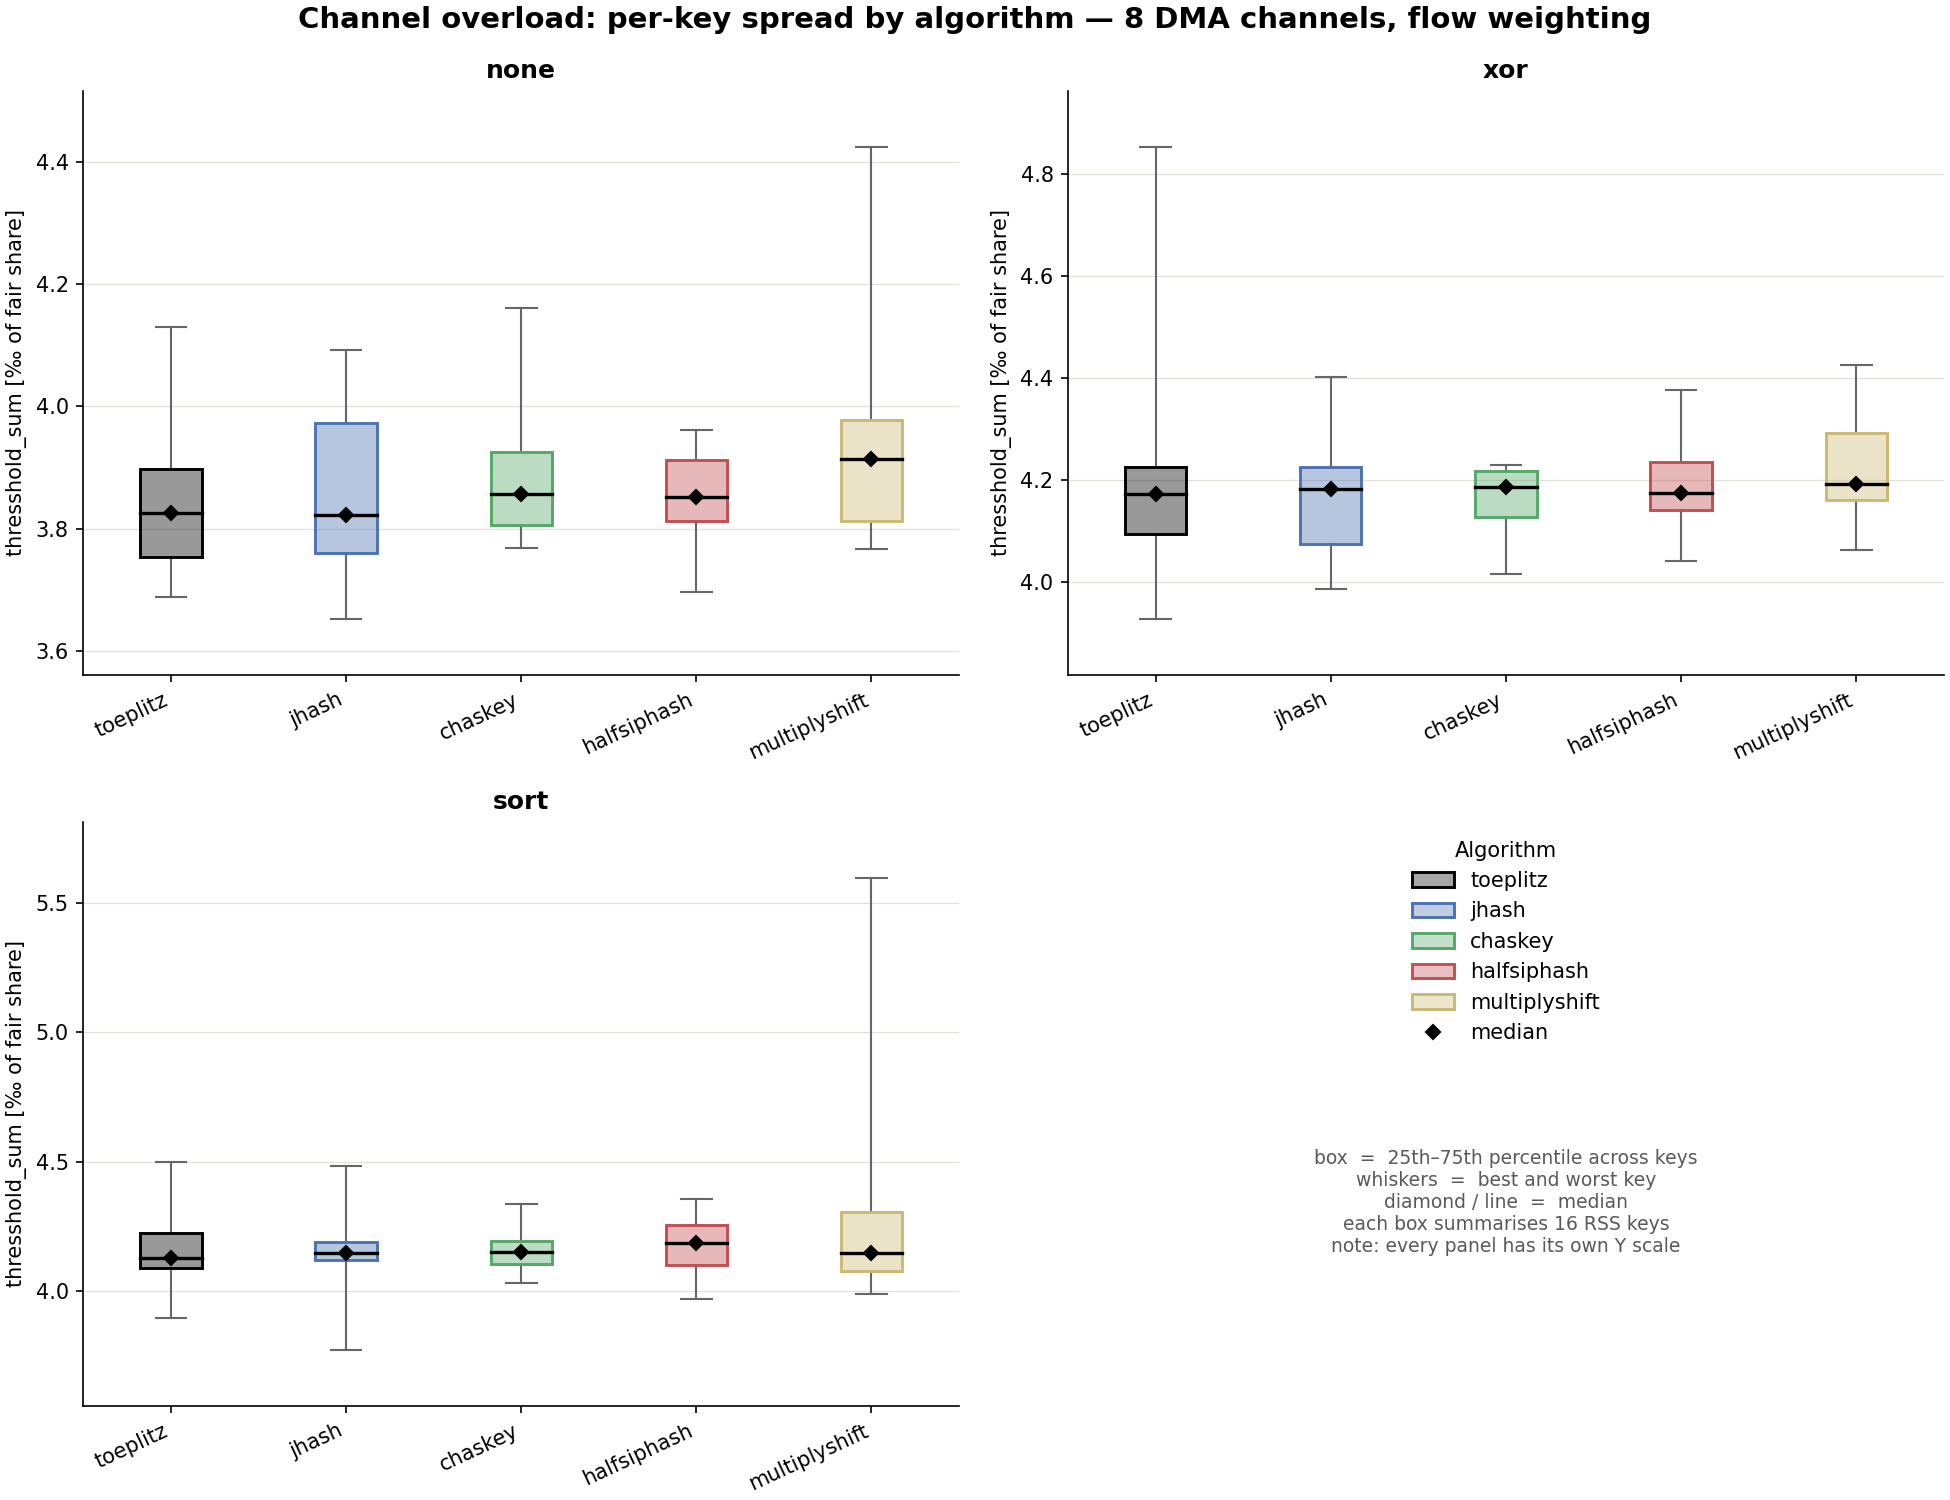
\includegraphics[width=\textwidth]{ostatne_vzorky/odid2_full_tuple/keys_8.png}
    \caption{8 kanálov}
  \end{subfigure}

  \begin{subfigure}{0.54\textwidth}
    \centering
    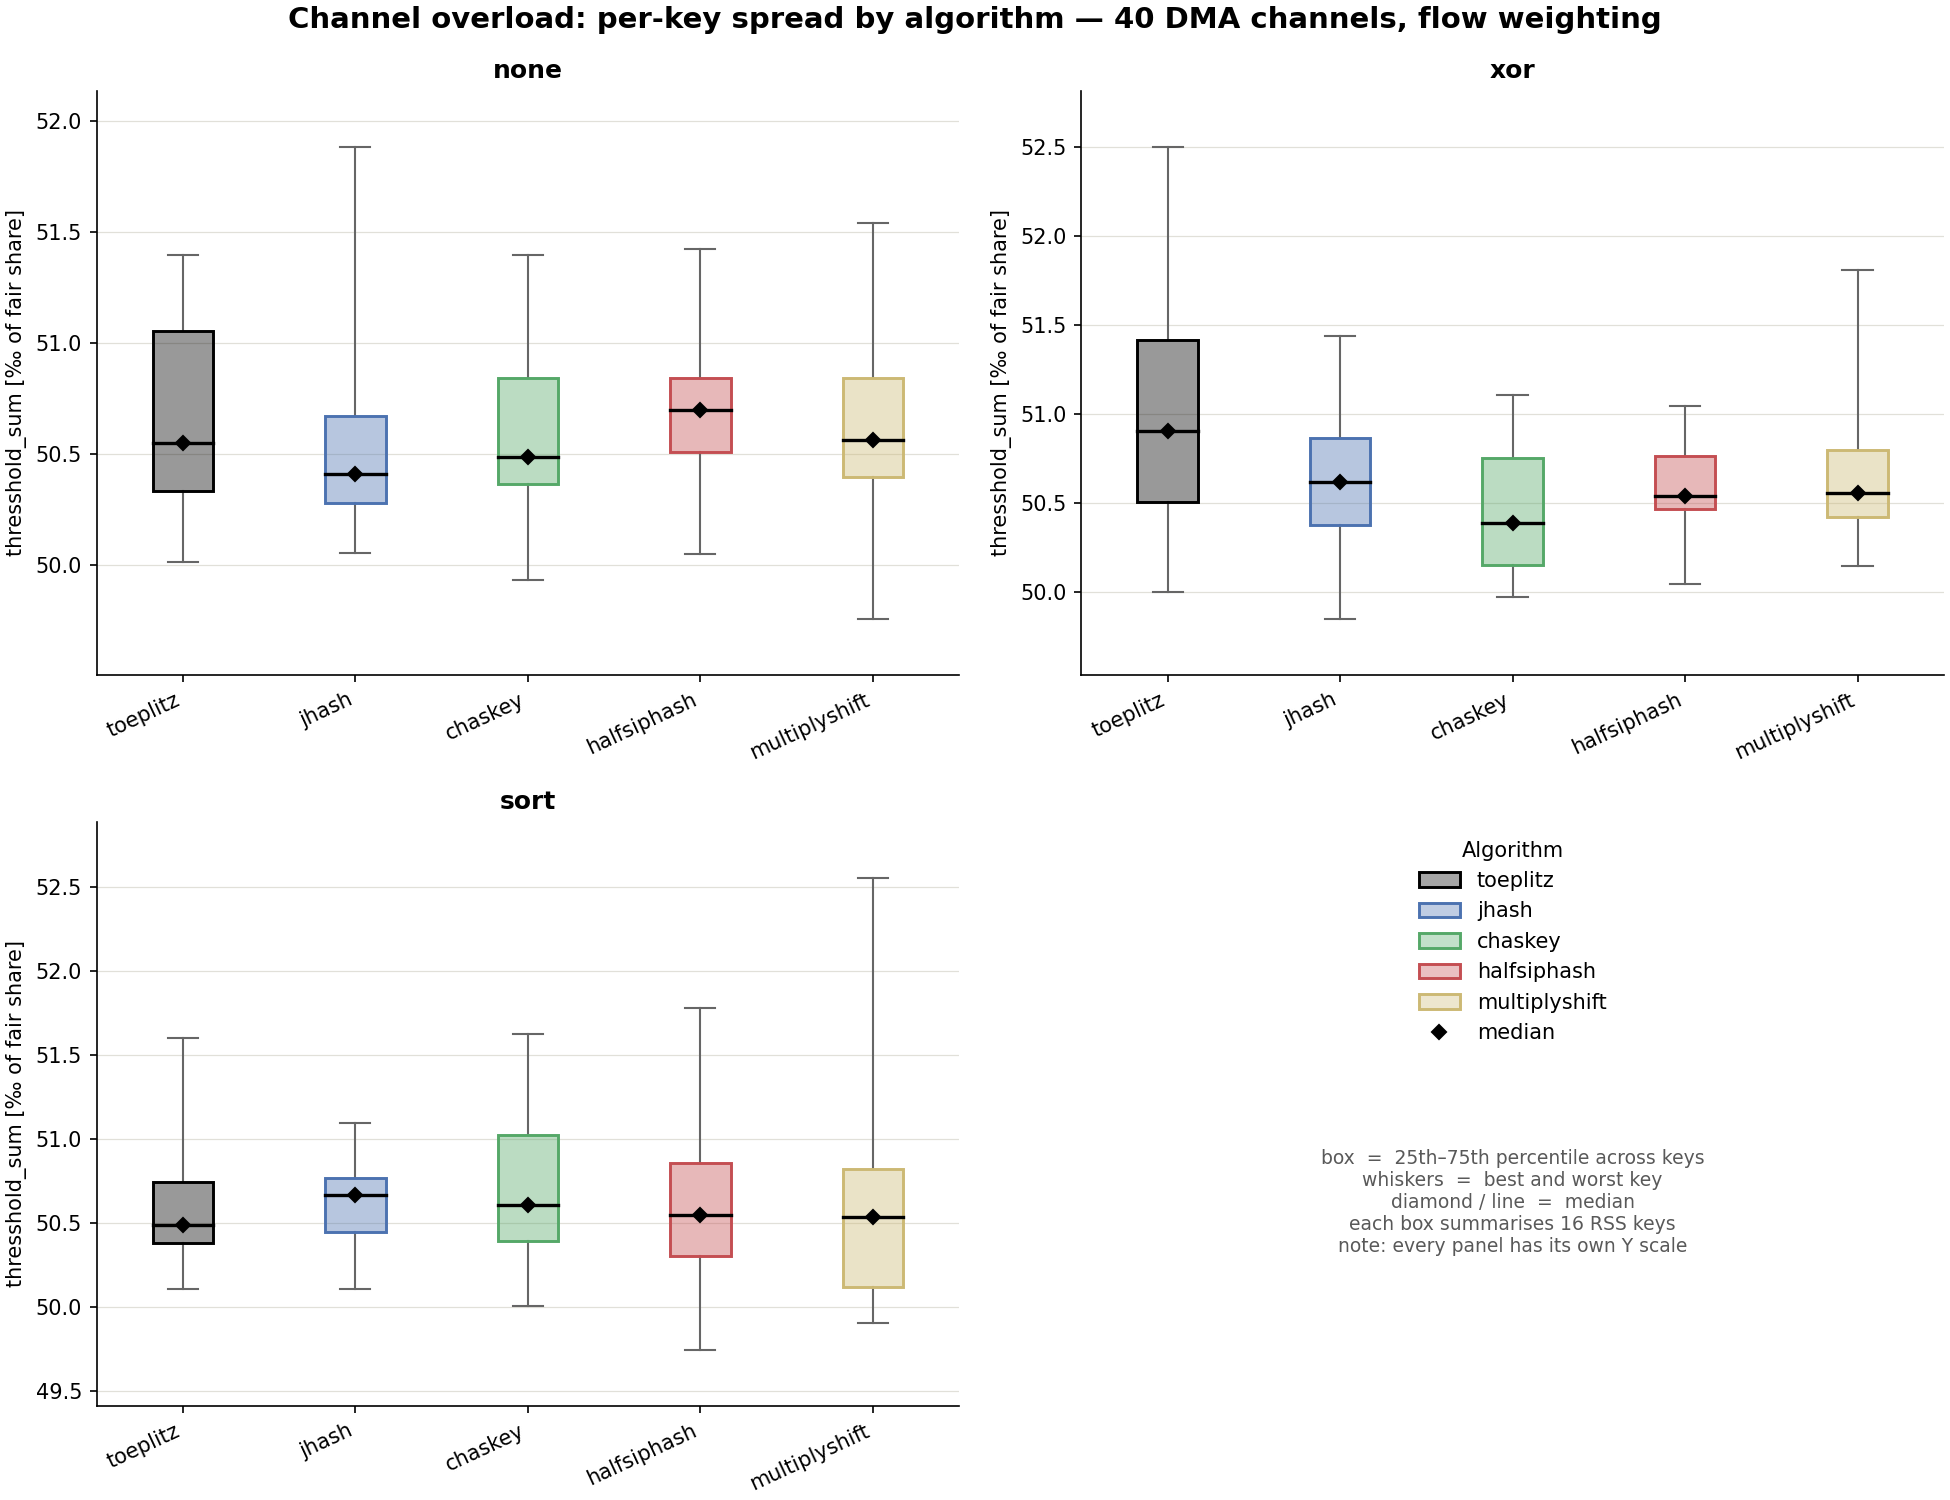
\includegraphics[width=\textwidth]{ostatne_vzorky/odid2_full_tuple/keys_40.png}
    \caption{40 kanálov}
  \end{subfigure}

  \begin{subfigure}{0.54\textwidth}
    \centering
    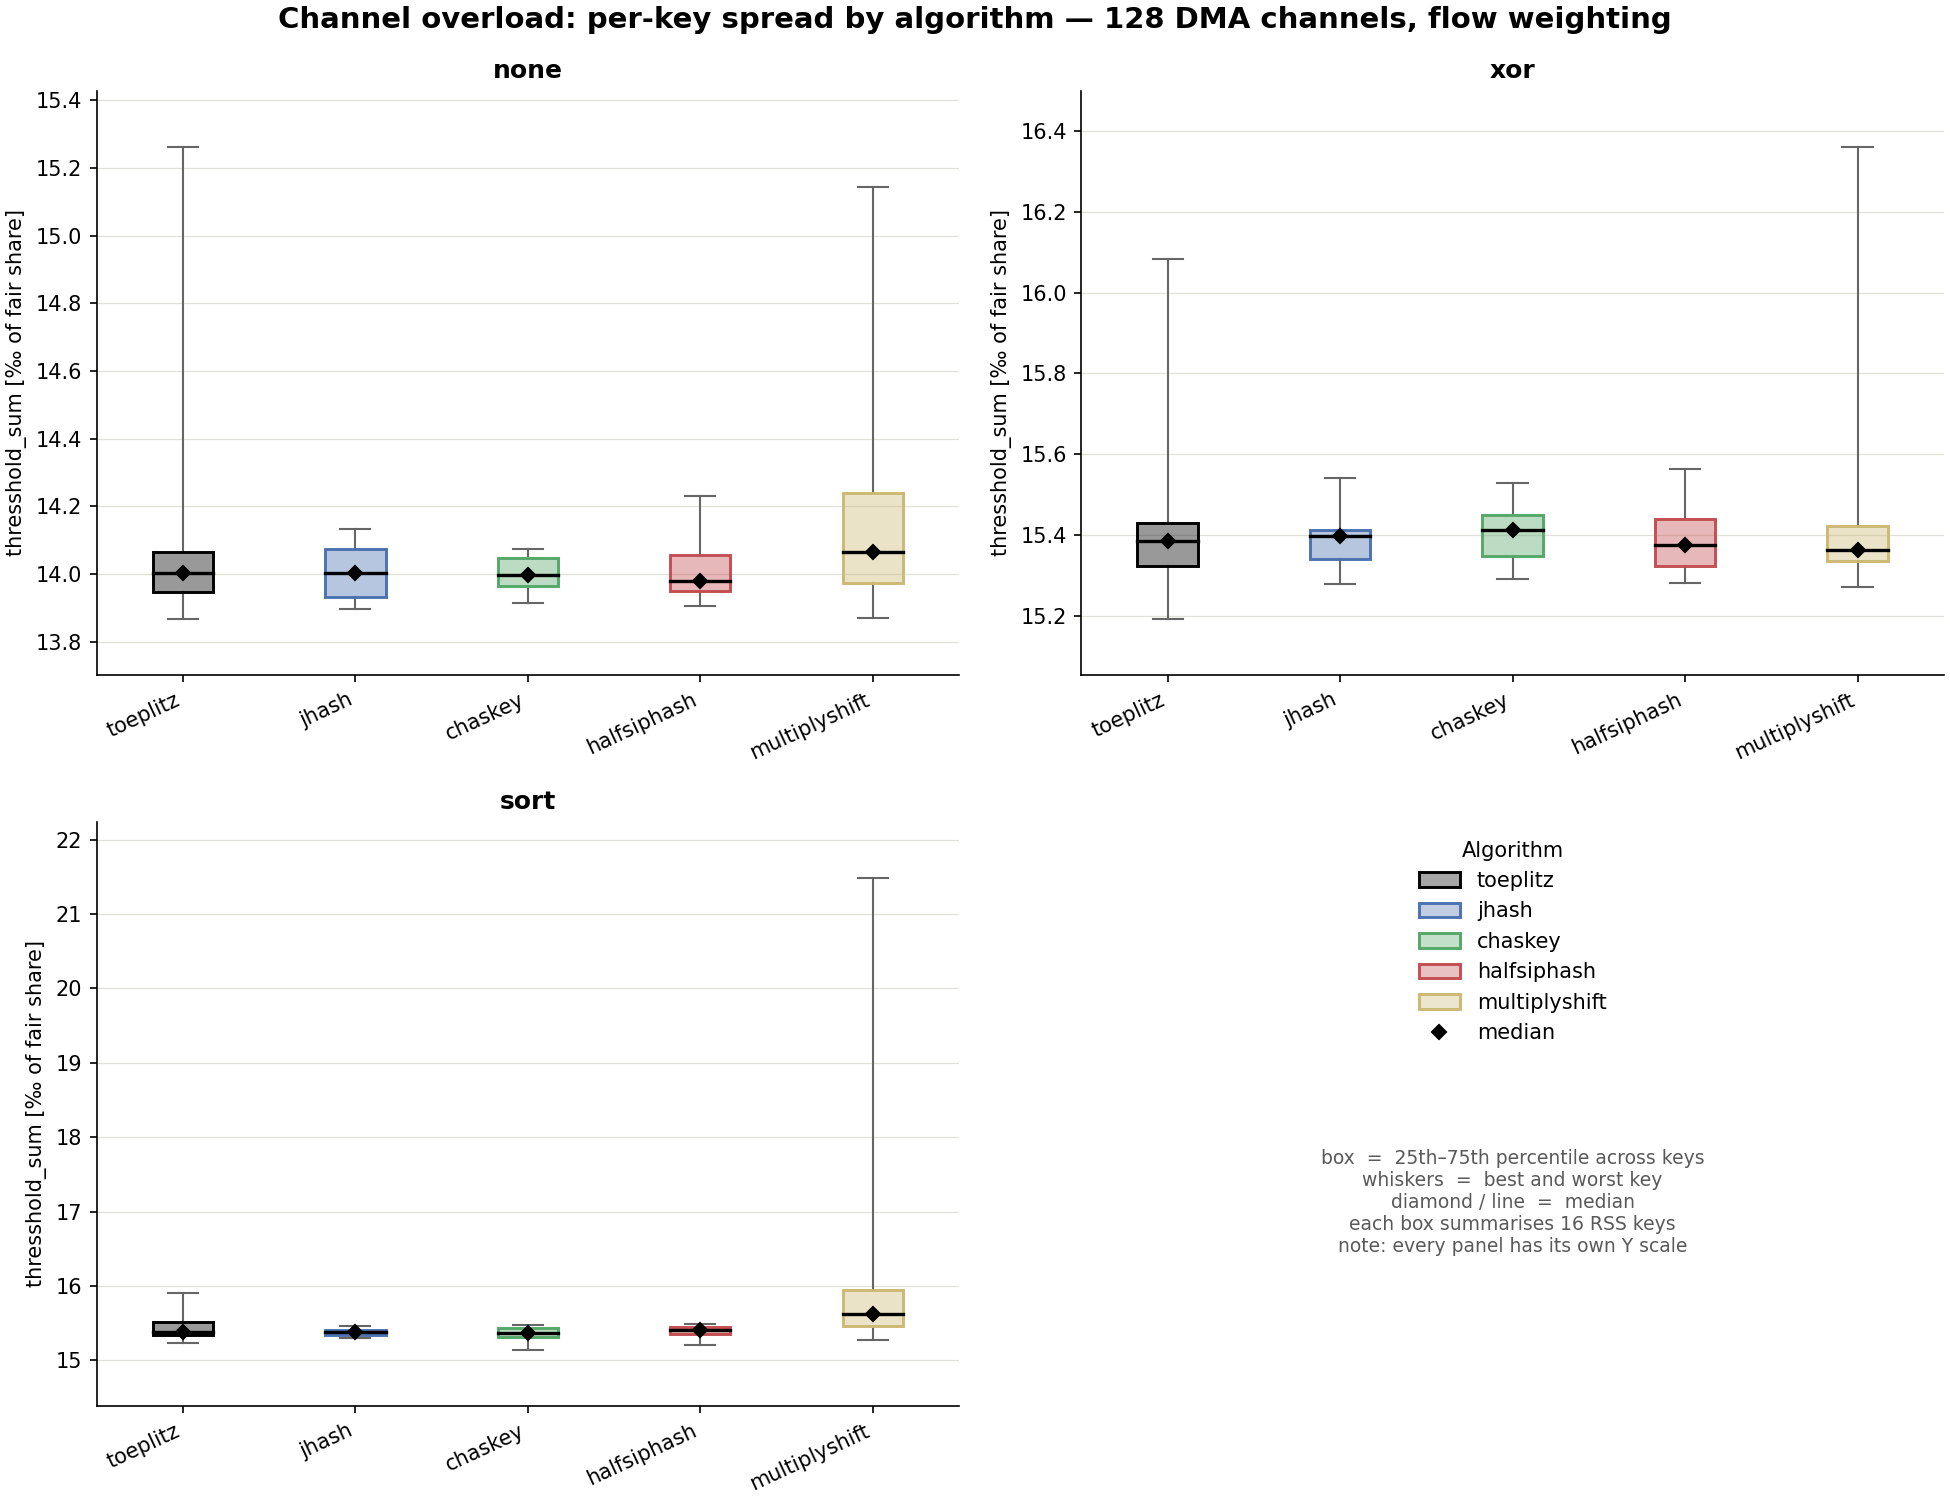
\includegraphics[width=\textwidth]{ostatne_vzorky/odid2_full_tuple/keys_128.png}
    \caption{128 kanálov}
  \end{subfigure}

  \caption{Rozptyl preťaženia medzi 16 kľúčmi pri váhe \texttt{flow}: \texttt{odid2}, plný tuple.}
  \label{fig:b-odid2-full-tuple-keys}
\end{figure}

\begin{figure}[ht]
  \centering
  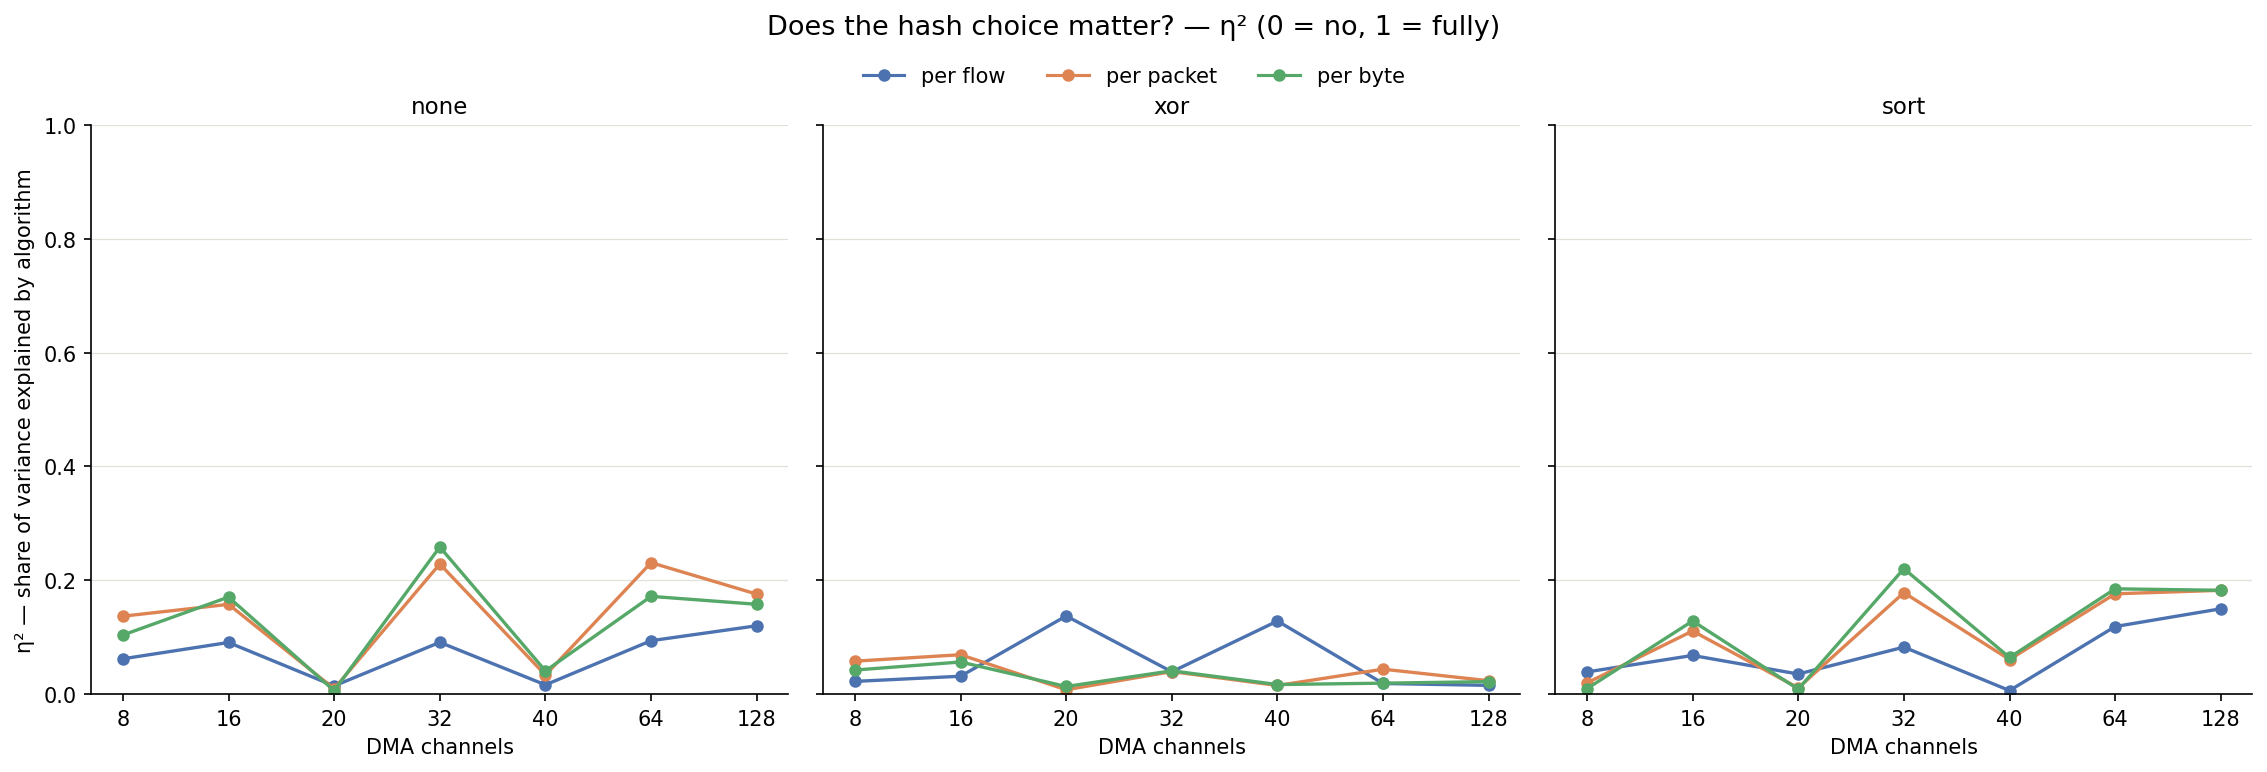
\includegraphics[width=0.9\textwidth]{ostatne_vzorky/odid2_full_tuple/spread.png}
  \caption{Podiel rozptylu vysvetlený voľbou funkcie ($\eta^2$): \texttt{odid2}, plný tuple.}
  \label{fig:b-odid2-full-tuple-spread}
\end{figure}

\clearpage
\begin{figure}[p]
  \centering
  \begin{subfigure}{0.60\textwidth}
    \centering
    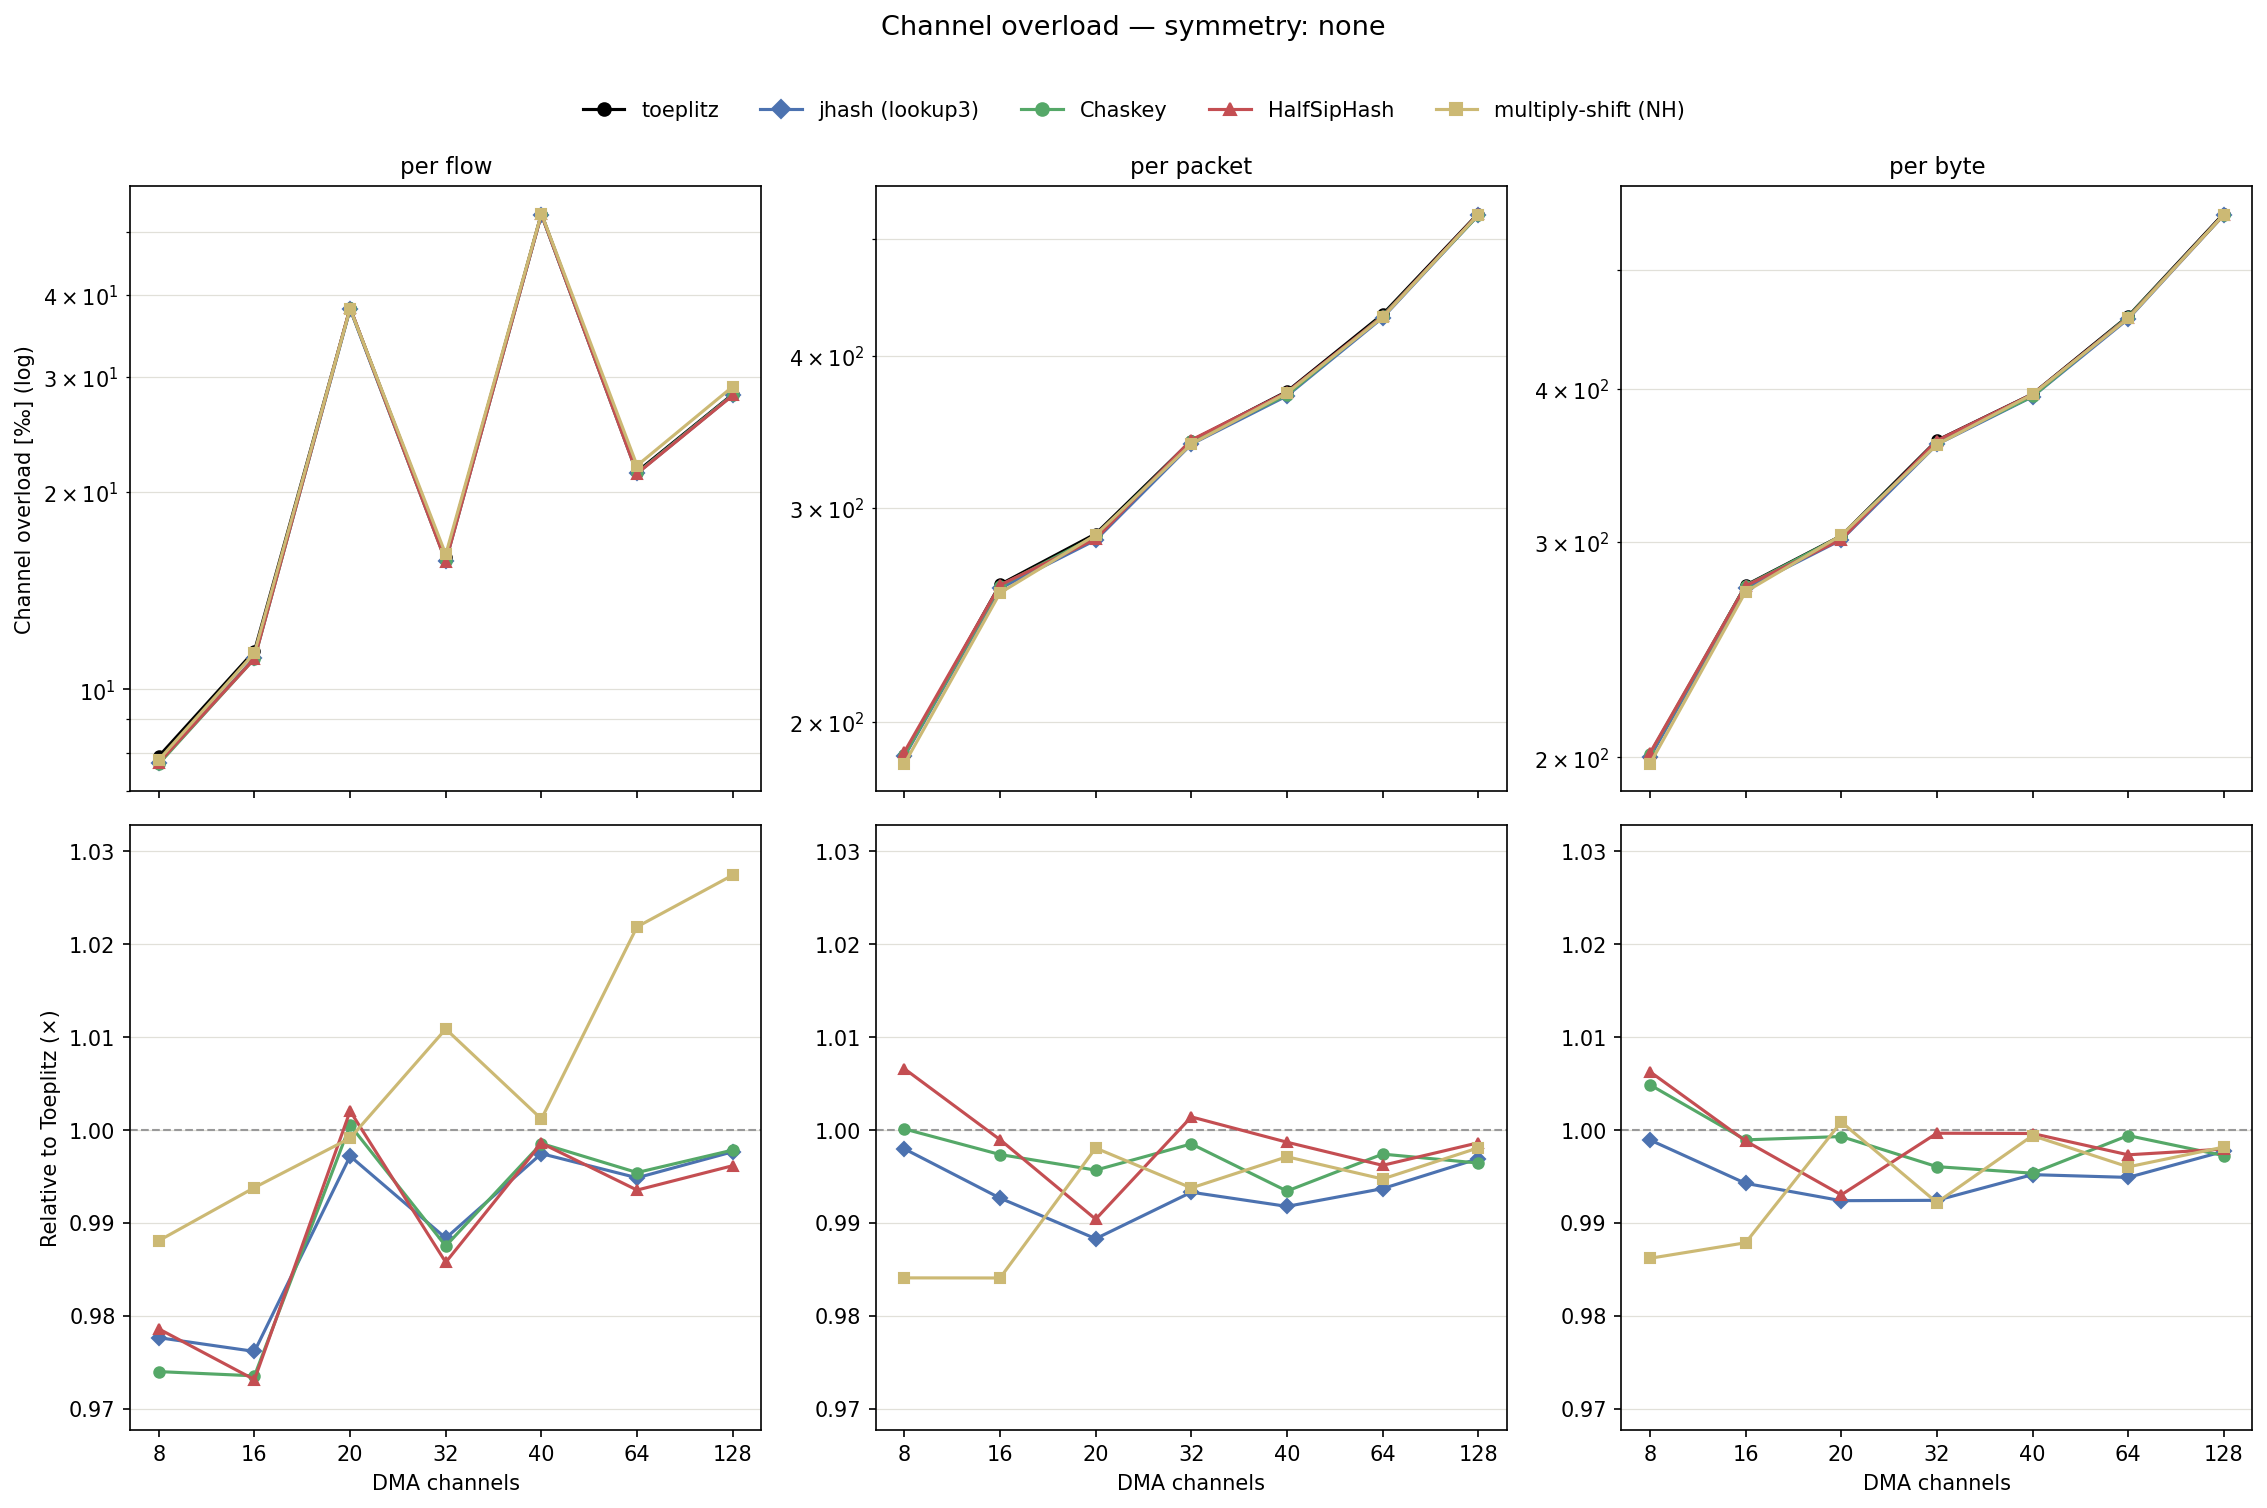
\includegraphics[width=\textwidth]{ostatne_vzorky/odid4_full_tuple/overload_none.png}
    \caption{bez symetrie}
  \end{subfigure}

  \begin{subfigure}{0.60\textwidth}
    \centering
    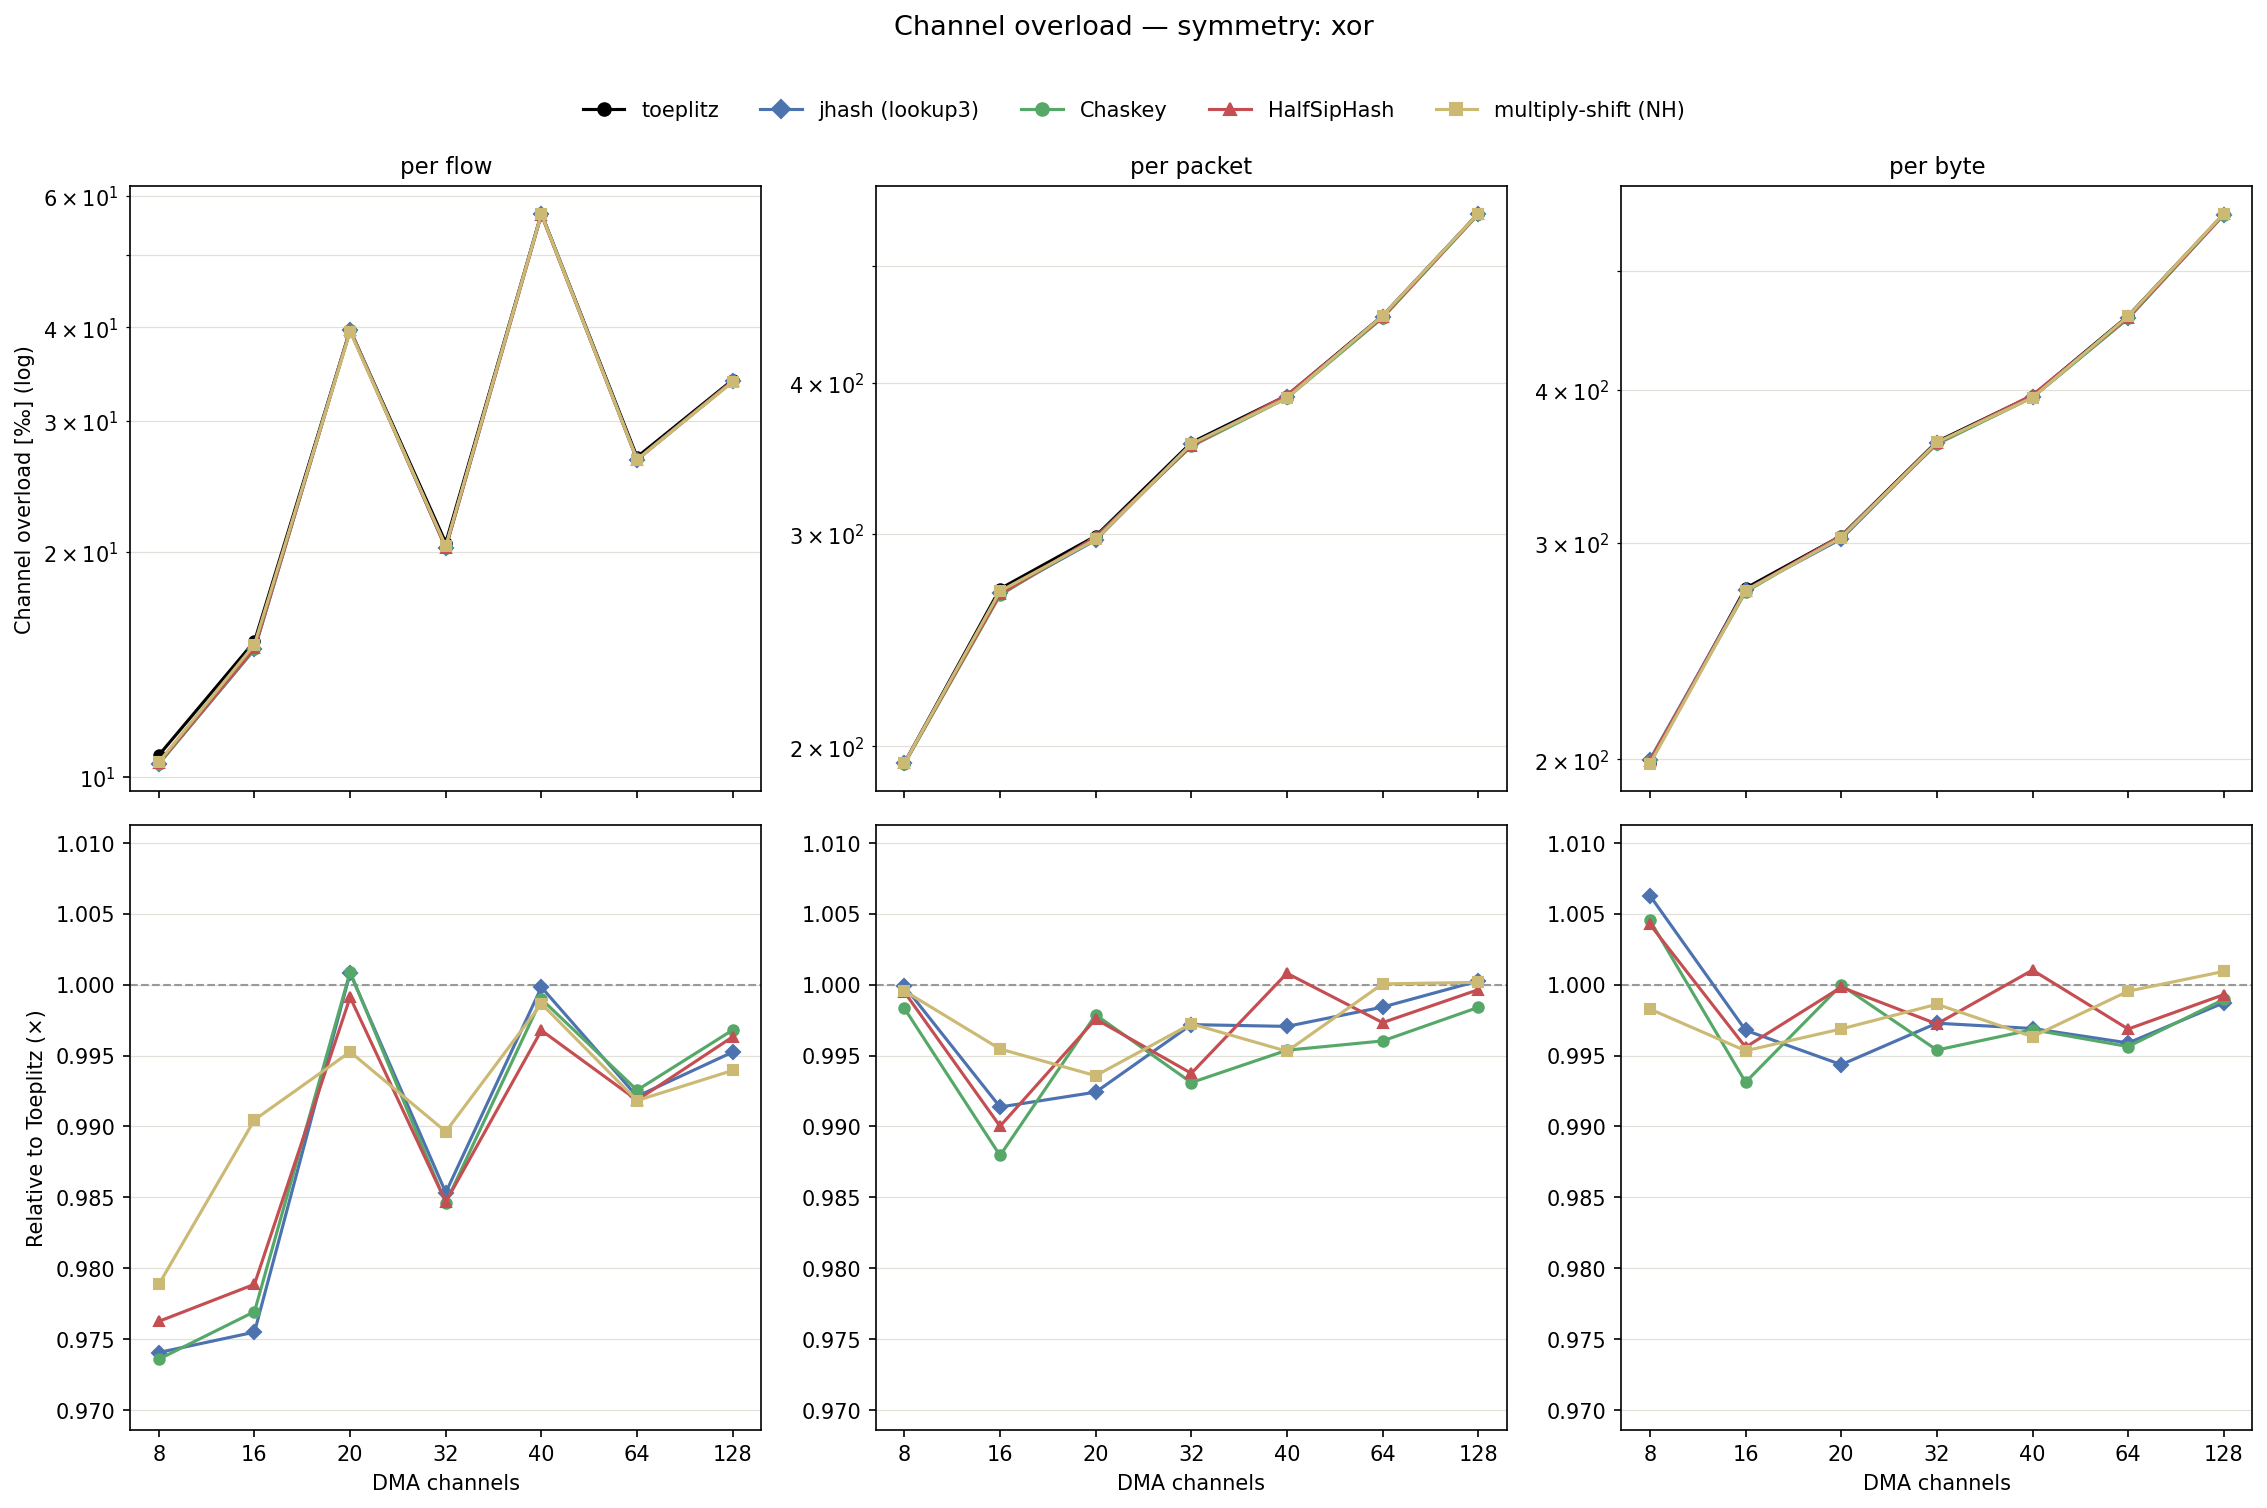
\includegraphics[width=\textwidth]{ostatne_vzorky/odid4_full_tuple/overload_xorfold.png}
    \caption{symetria XOR}
  \end{subfigure}

  \begin{subfigure}{0.60\textwidth}
    \centering
    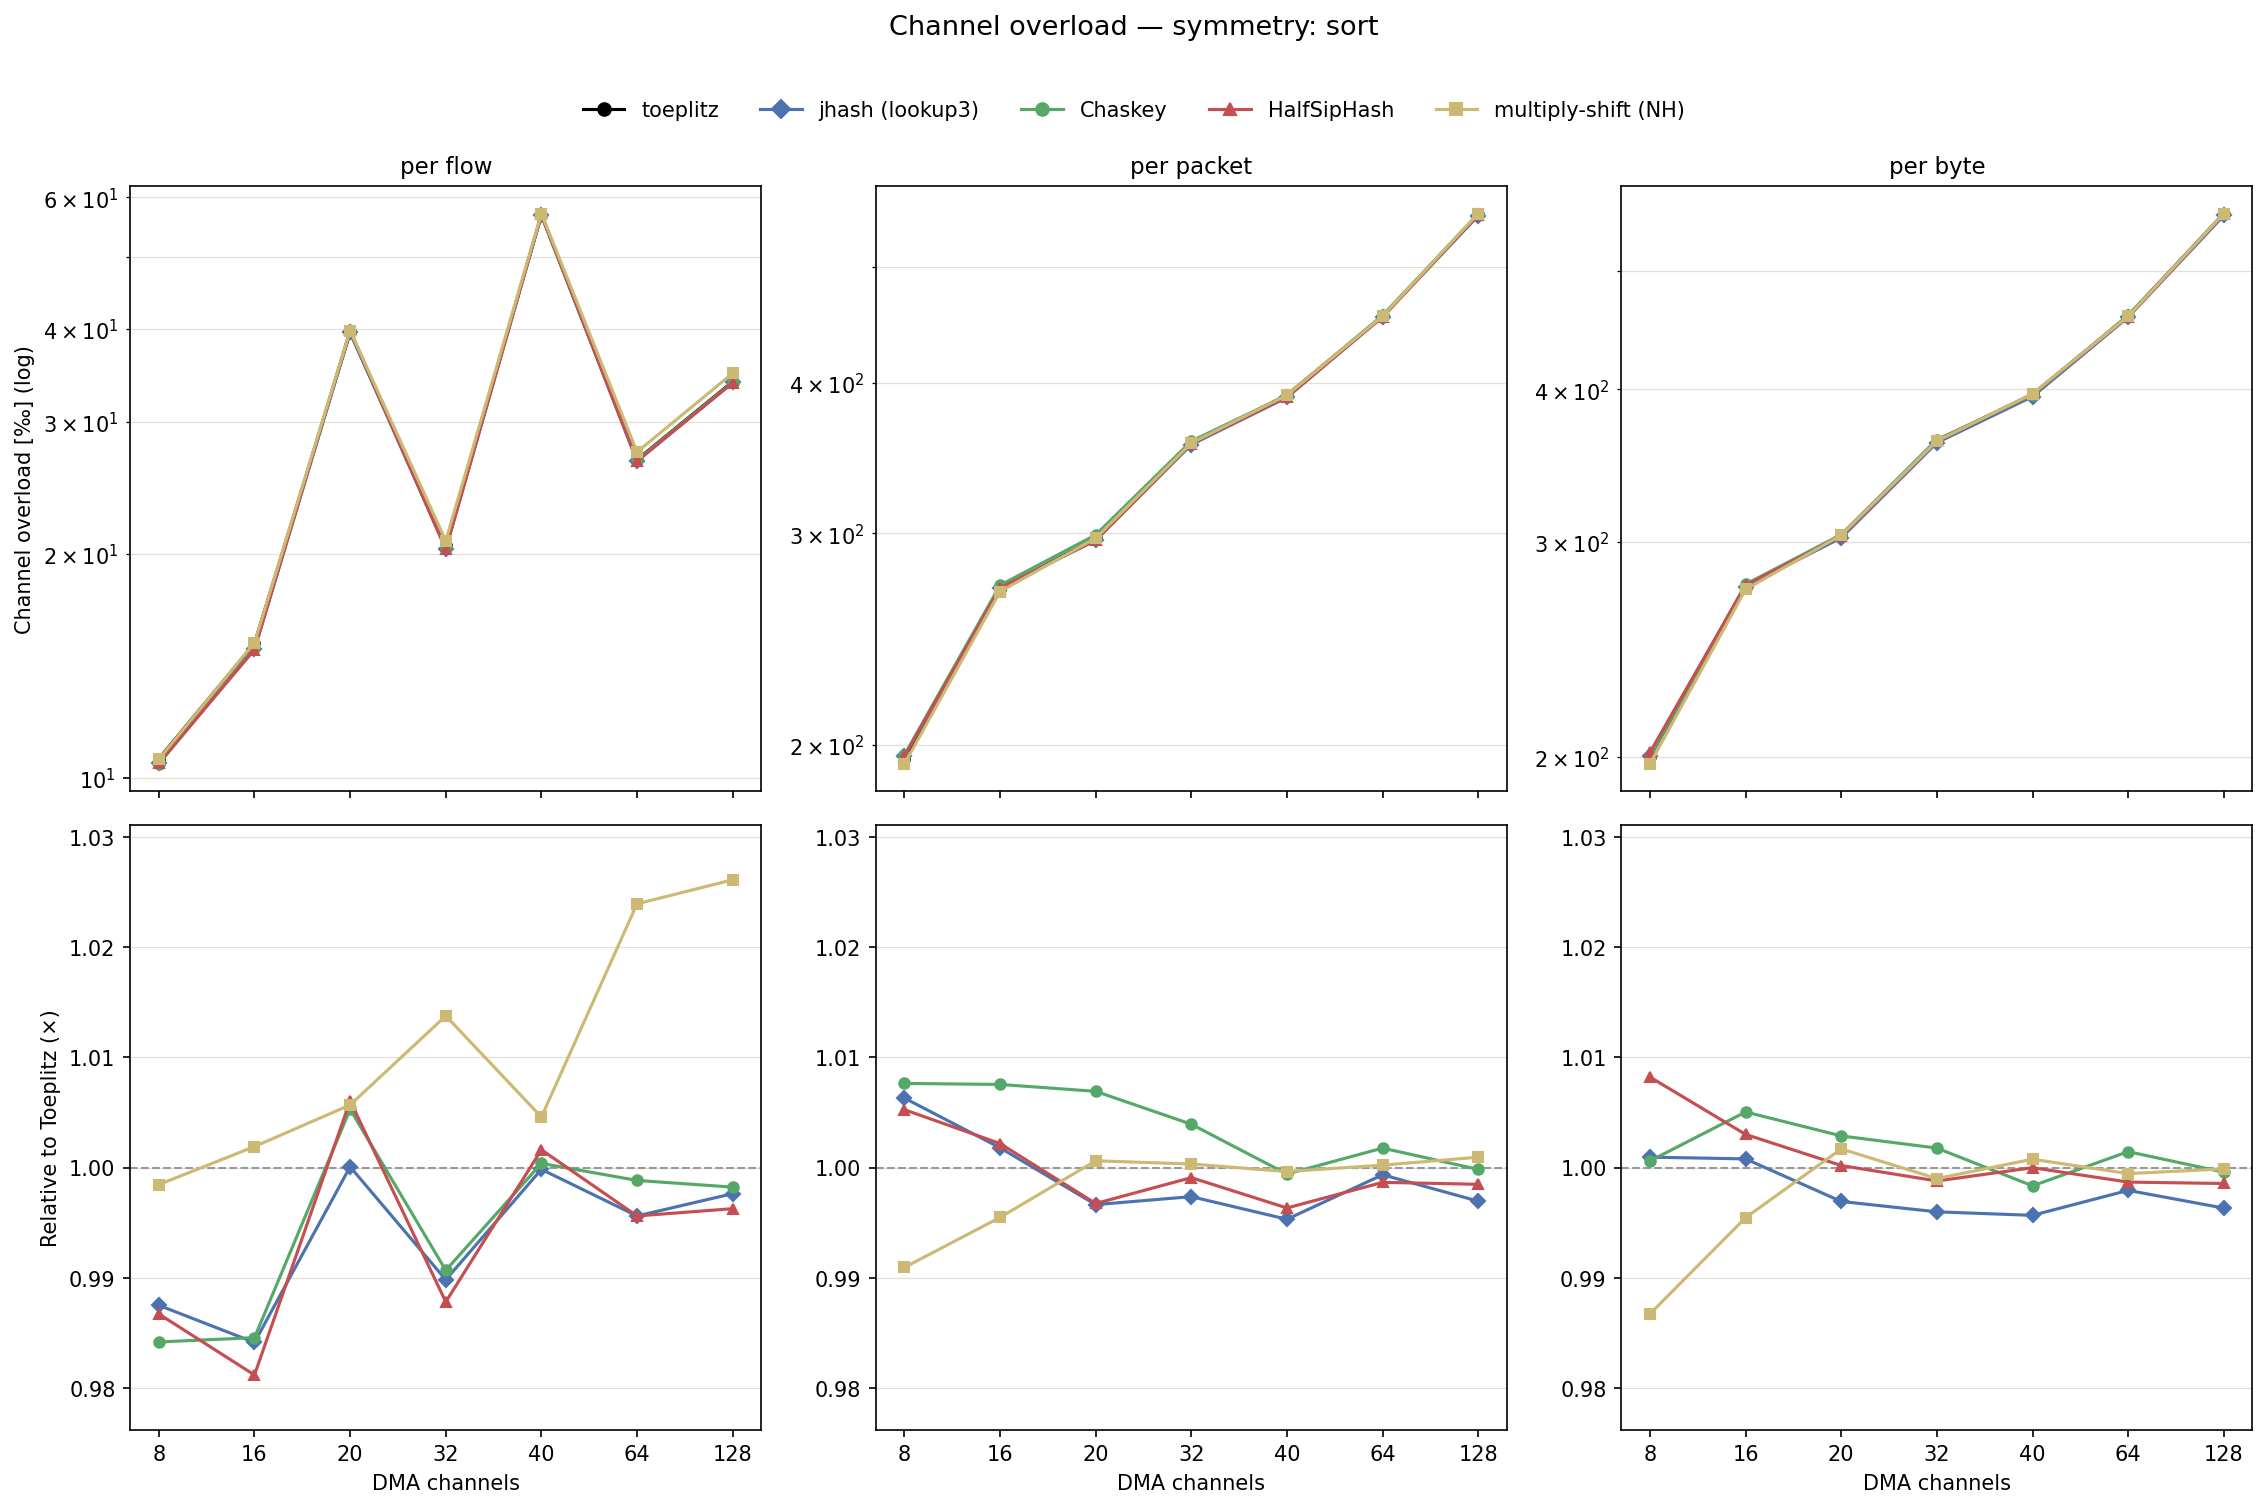
\includegraphics[width=\textwidth]{ostatne_vzorky/odid4_full_tuple/overload_sortfold.png}
    \caption{symetria sort}
  \end{subfigure}

  \caption{Preťaženie funkcií a pomer k~Toeplitzu: \texttt{odid4}, plný tuple.}
  \label{fig:b-odid4-full-tuple-overload}
\end{figure}

\begin{figure}[p]
  \centering
  \begin{subfigure}{0.54\textwidth}
    \centering
    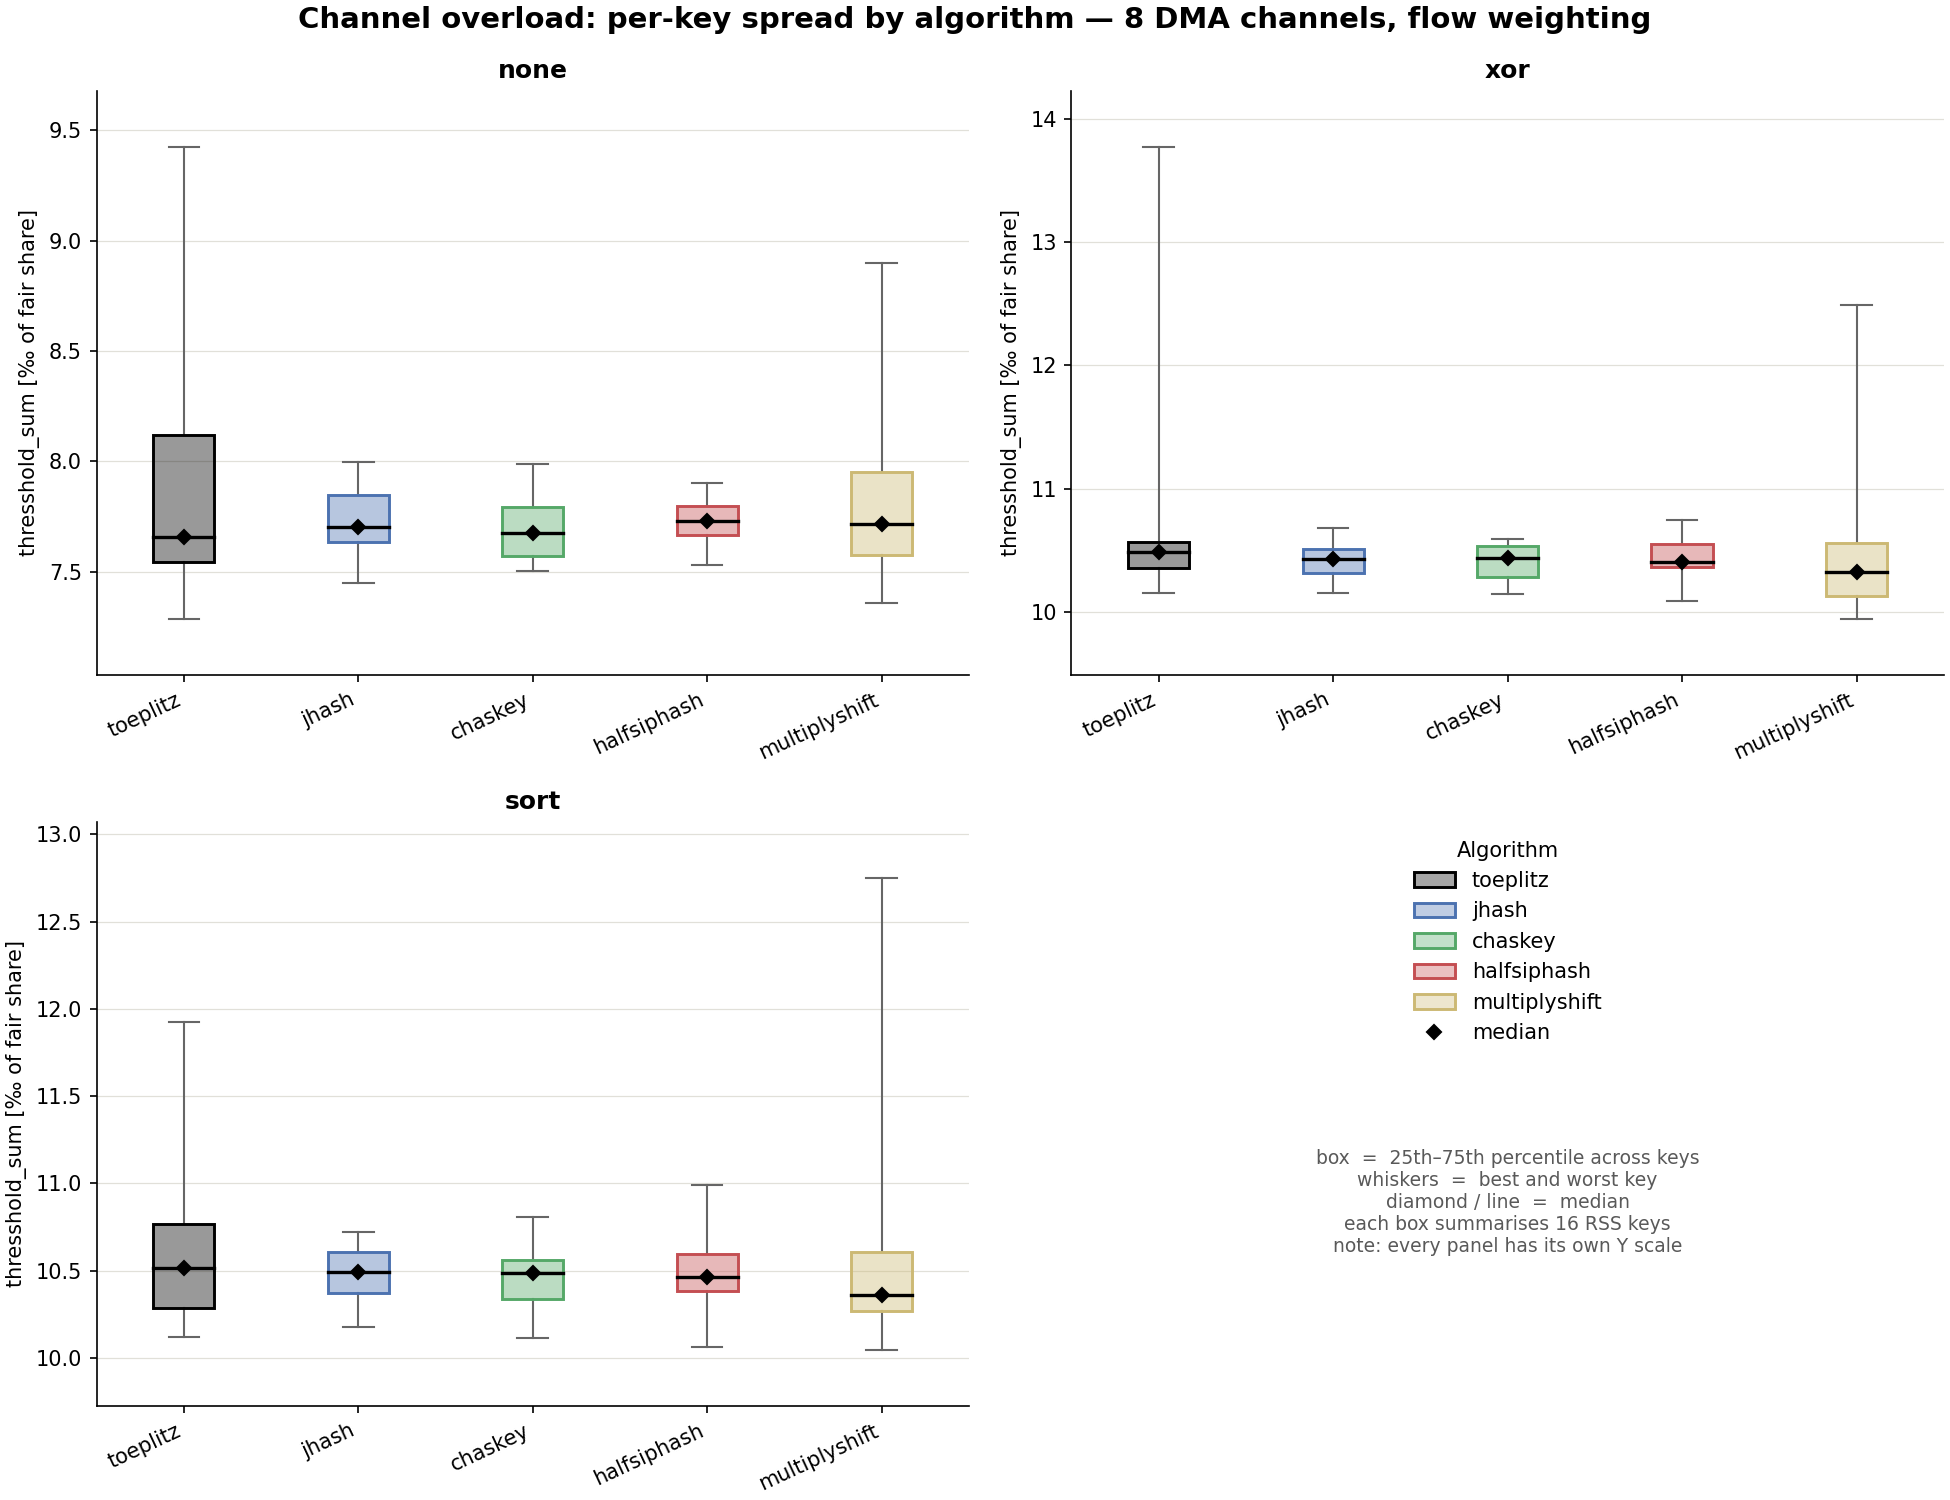
\includegraphics[width=\textwidth]{ostatne_vzorky/odid4_full_tuple/keys_8.png}
    \caption{8 kanálov}
  \end{subfigure}

  \begin{subfigure}{0.54\textwidth}
    \centering
    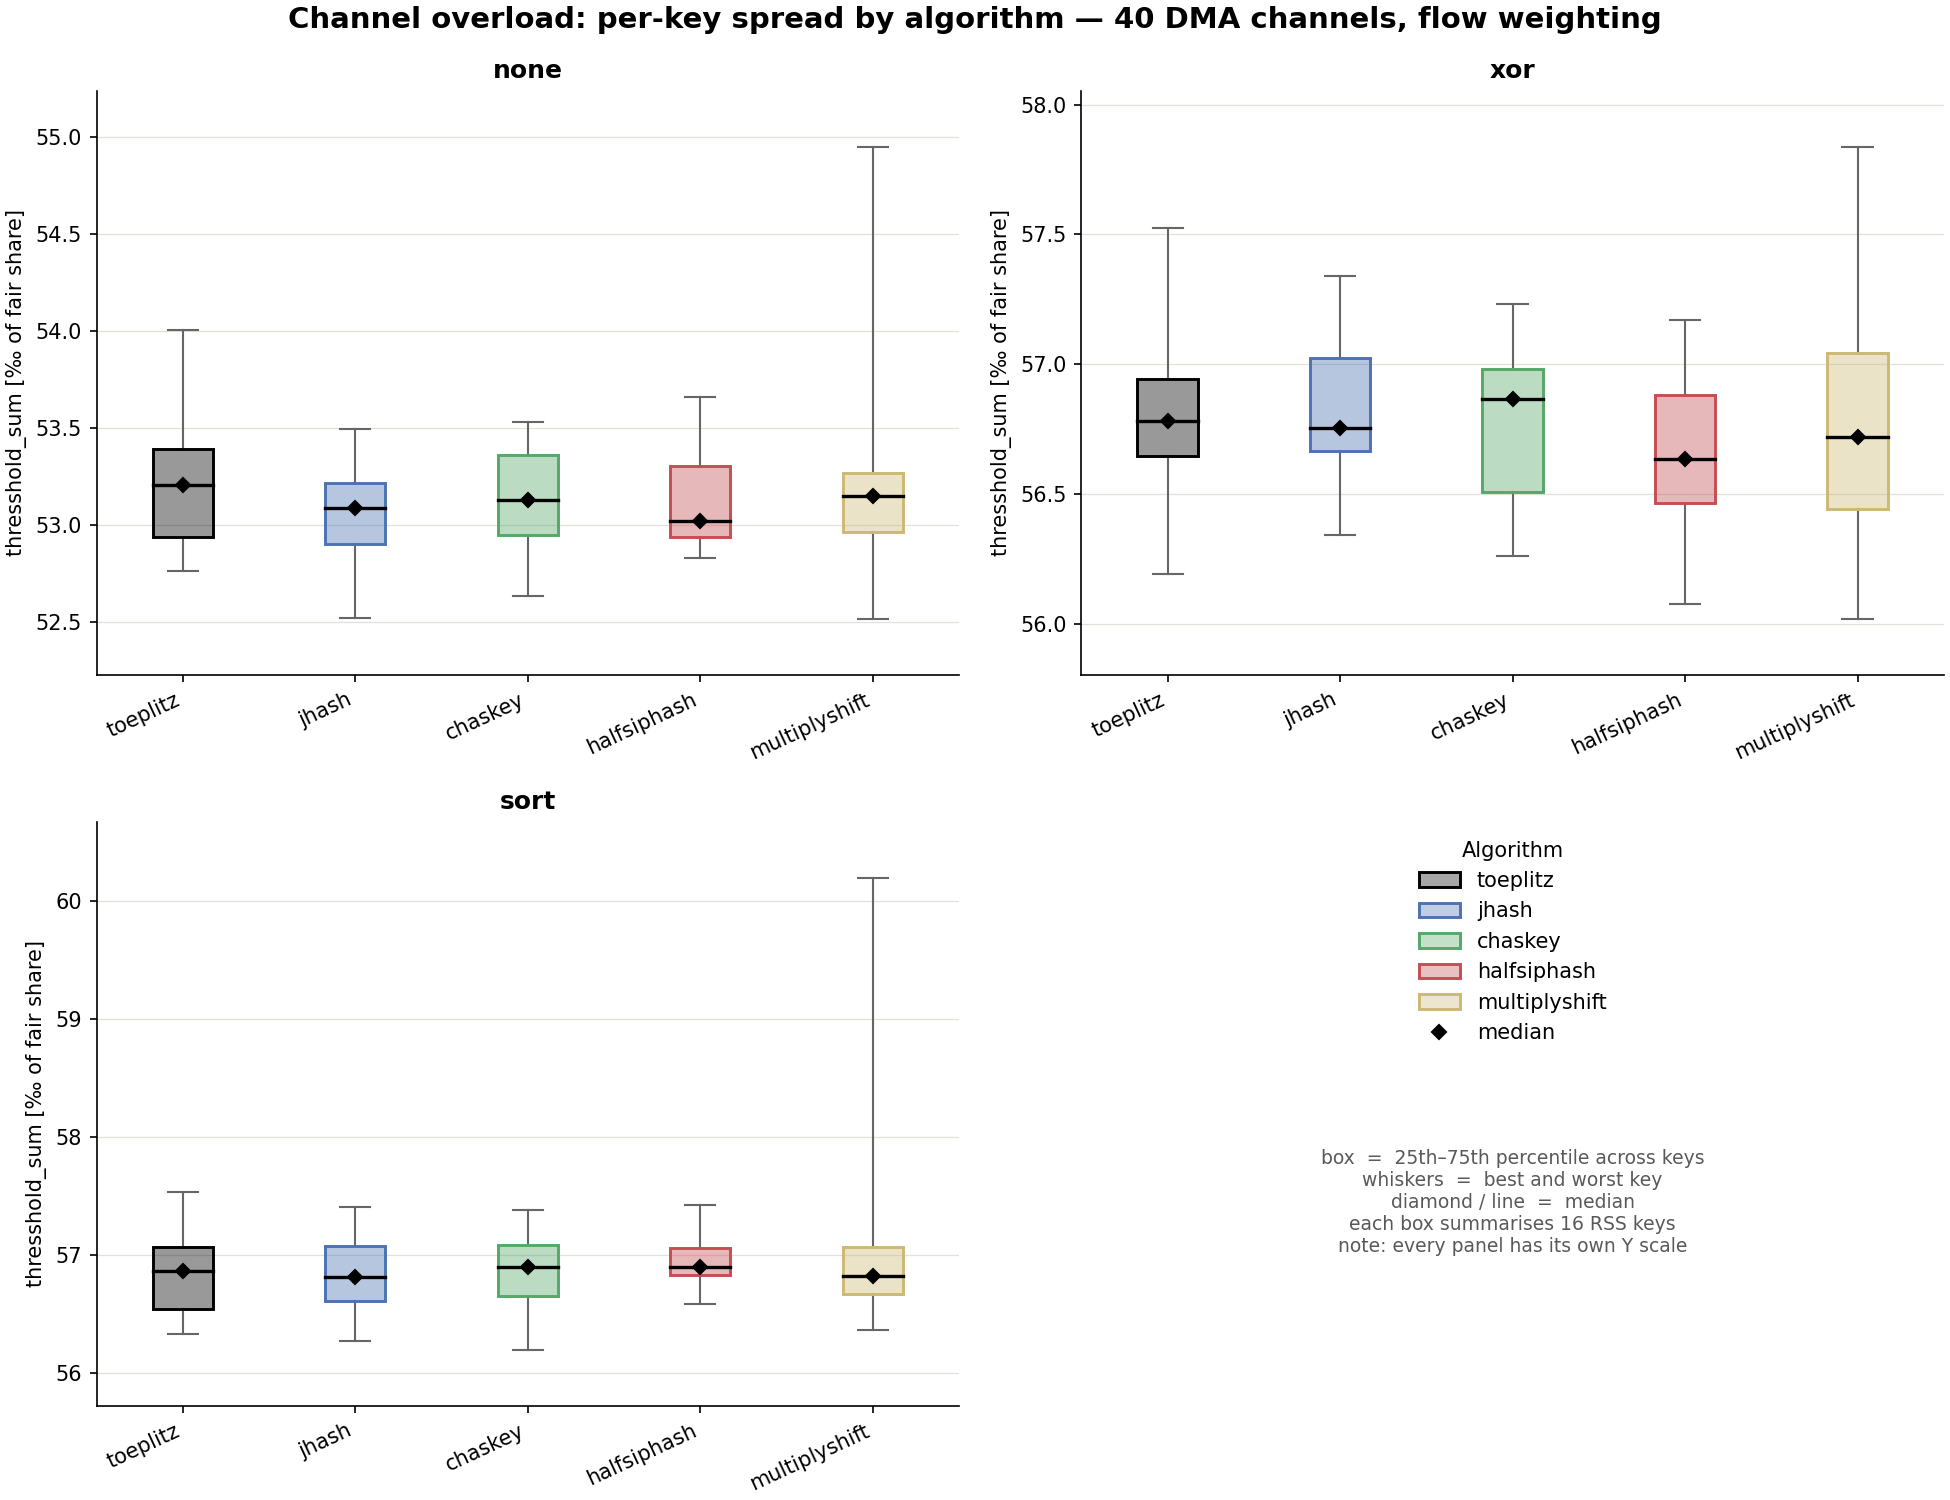
\includegraphics[width=\textwidth]{ostatne_vzorky/odid4_full_tuple/keys_40.png}
    \caption{40 kanálov}
  \end{subfigure}

  \begin{subfigure}{0.54\textwidth}
    \centering
    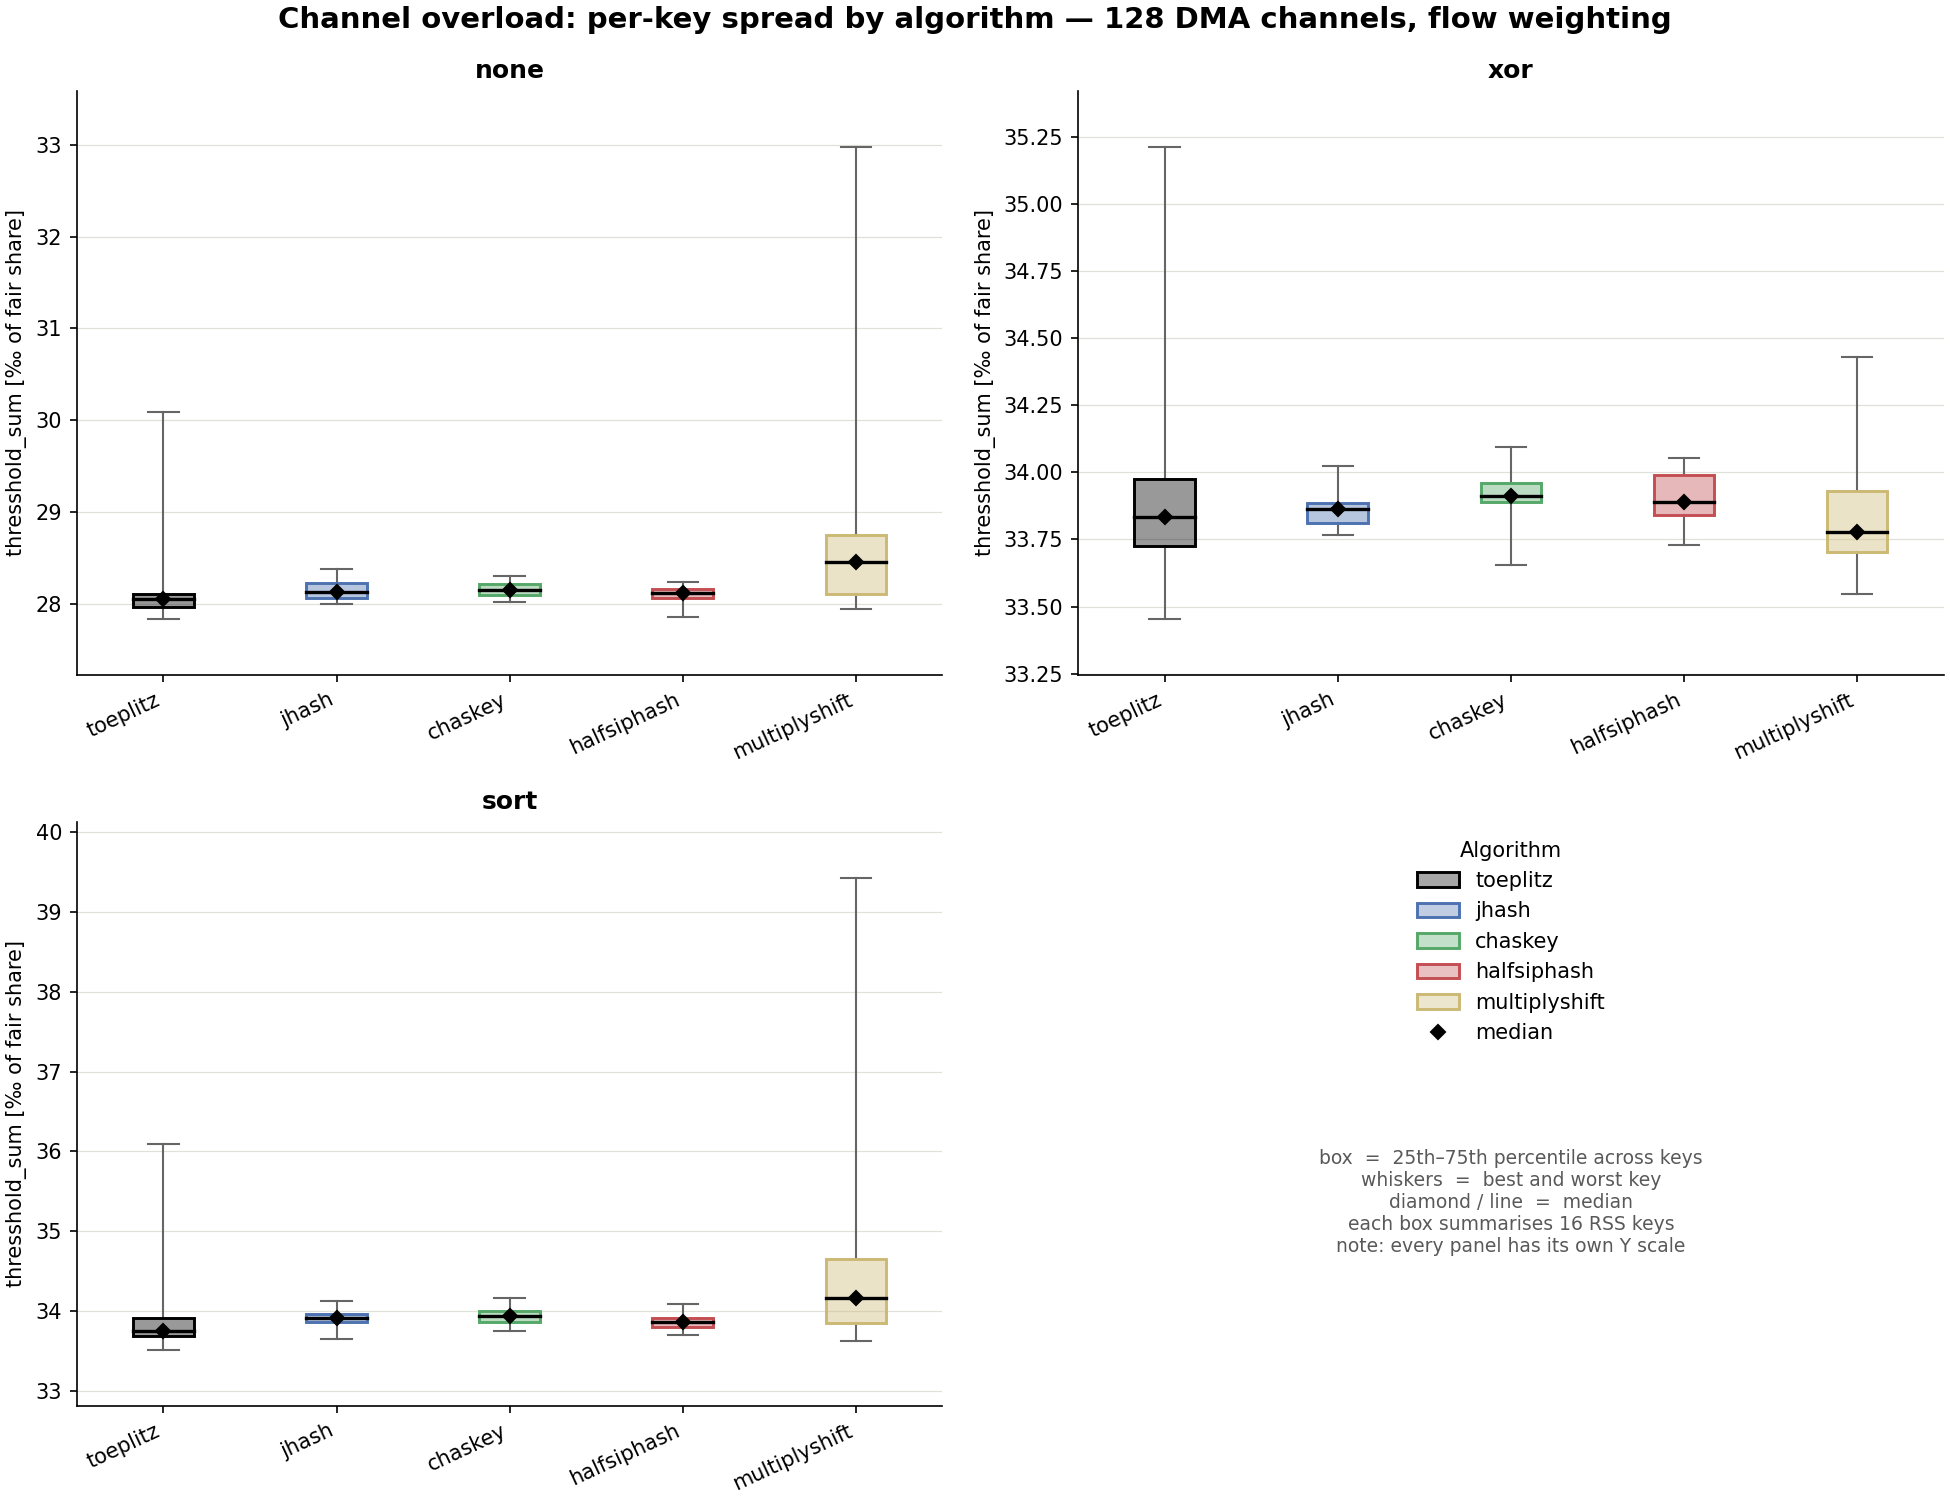
\includegraphics[width=\textwidth]{ostatne_vzorky/odid4_full_tuple/keys_128.png}
    \caption{128 kanálov}
  \end{subfigure}

  \caption{Rozptyl preťaženia medzi 16 kľúčmi pri váhe \texttt{flow}: \texttt{odid4}, plný tuple.}
  \label{fig:b-odid4-full-tuple-keys}
\end{figure}

\begin{figure}[ht]
  \centering
  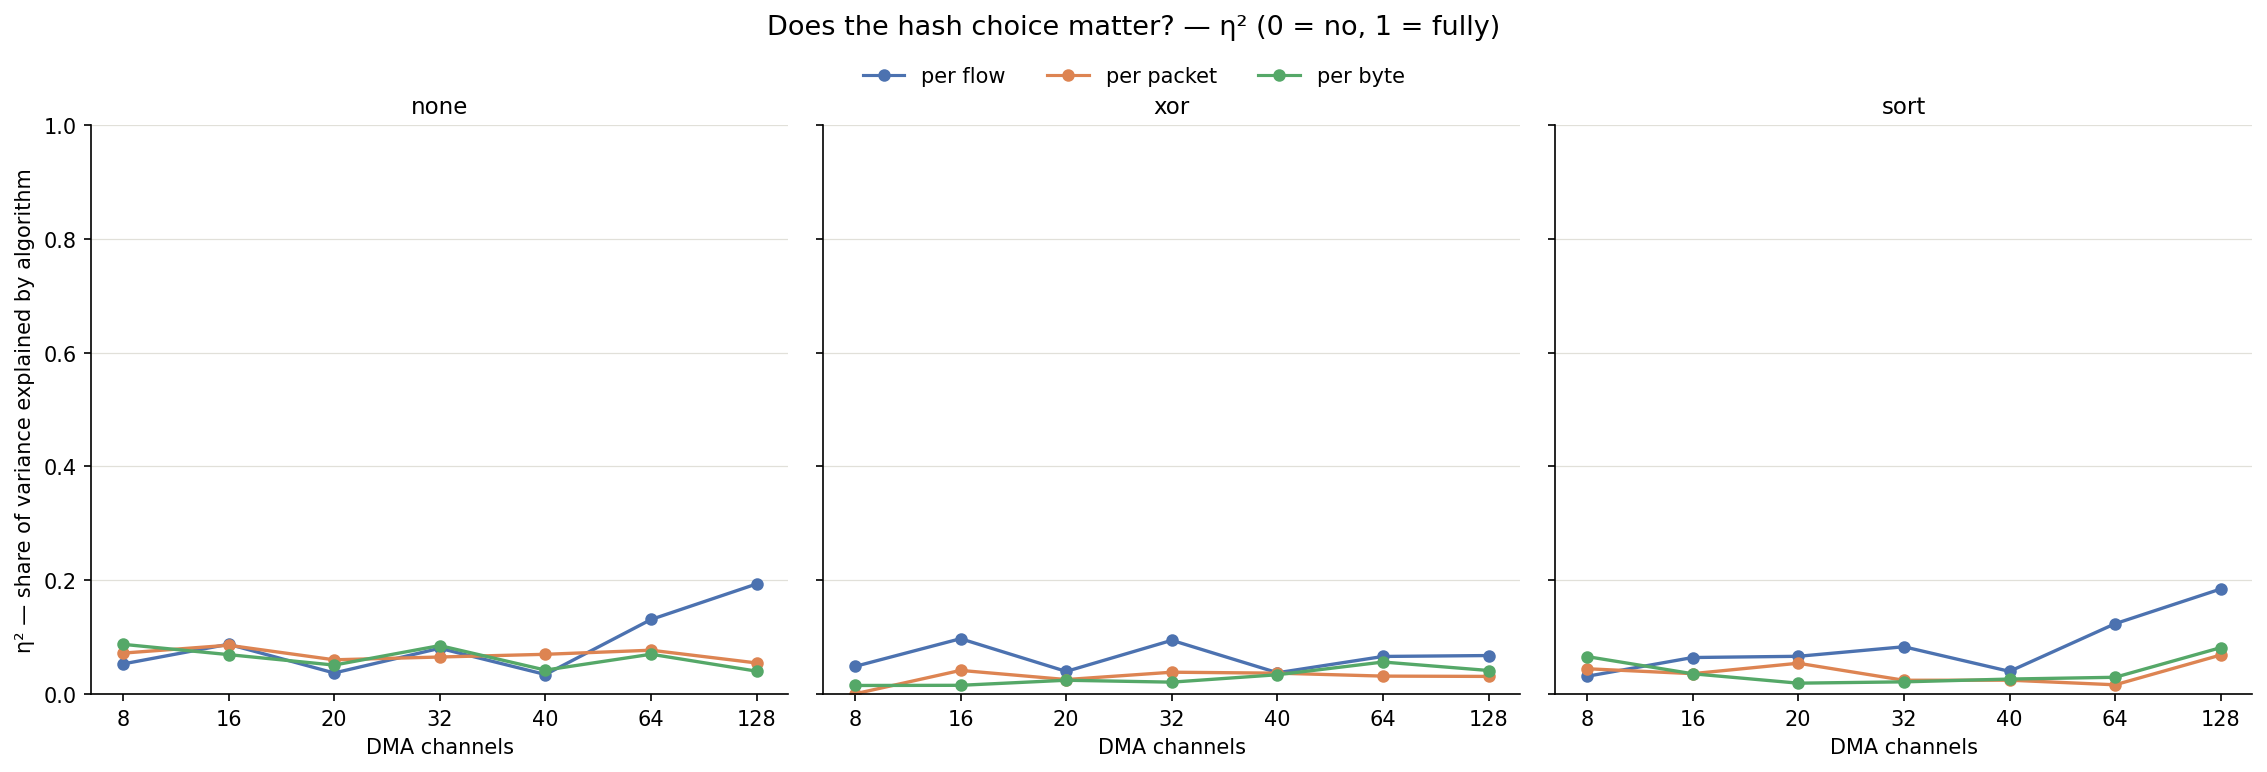
\includegraphics[width=0.9\textwidth]{ostatne_vzorky/odid4_full_tuple/spread.png}
  \caption{Podiel rozptylu vysvetlený voľbou funkcie ($\eta^2$): \texttt{odid4}, plný tuple.}
  \label{fig:b-odid4-full-tuple-spread}
\end{figure}

\clearpage
\begin{figure}[p]
  \centering
  \begin{subfigure}{0.60\textwidth}
    \centering
    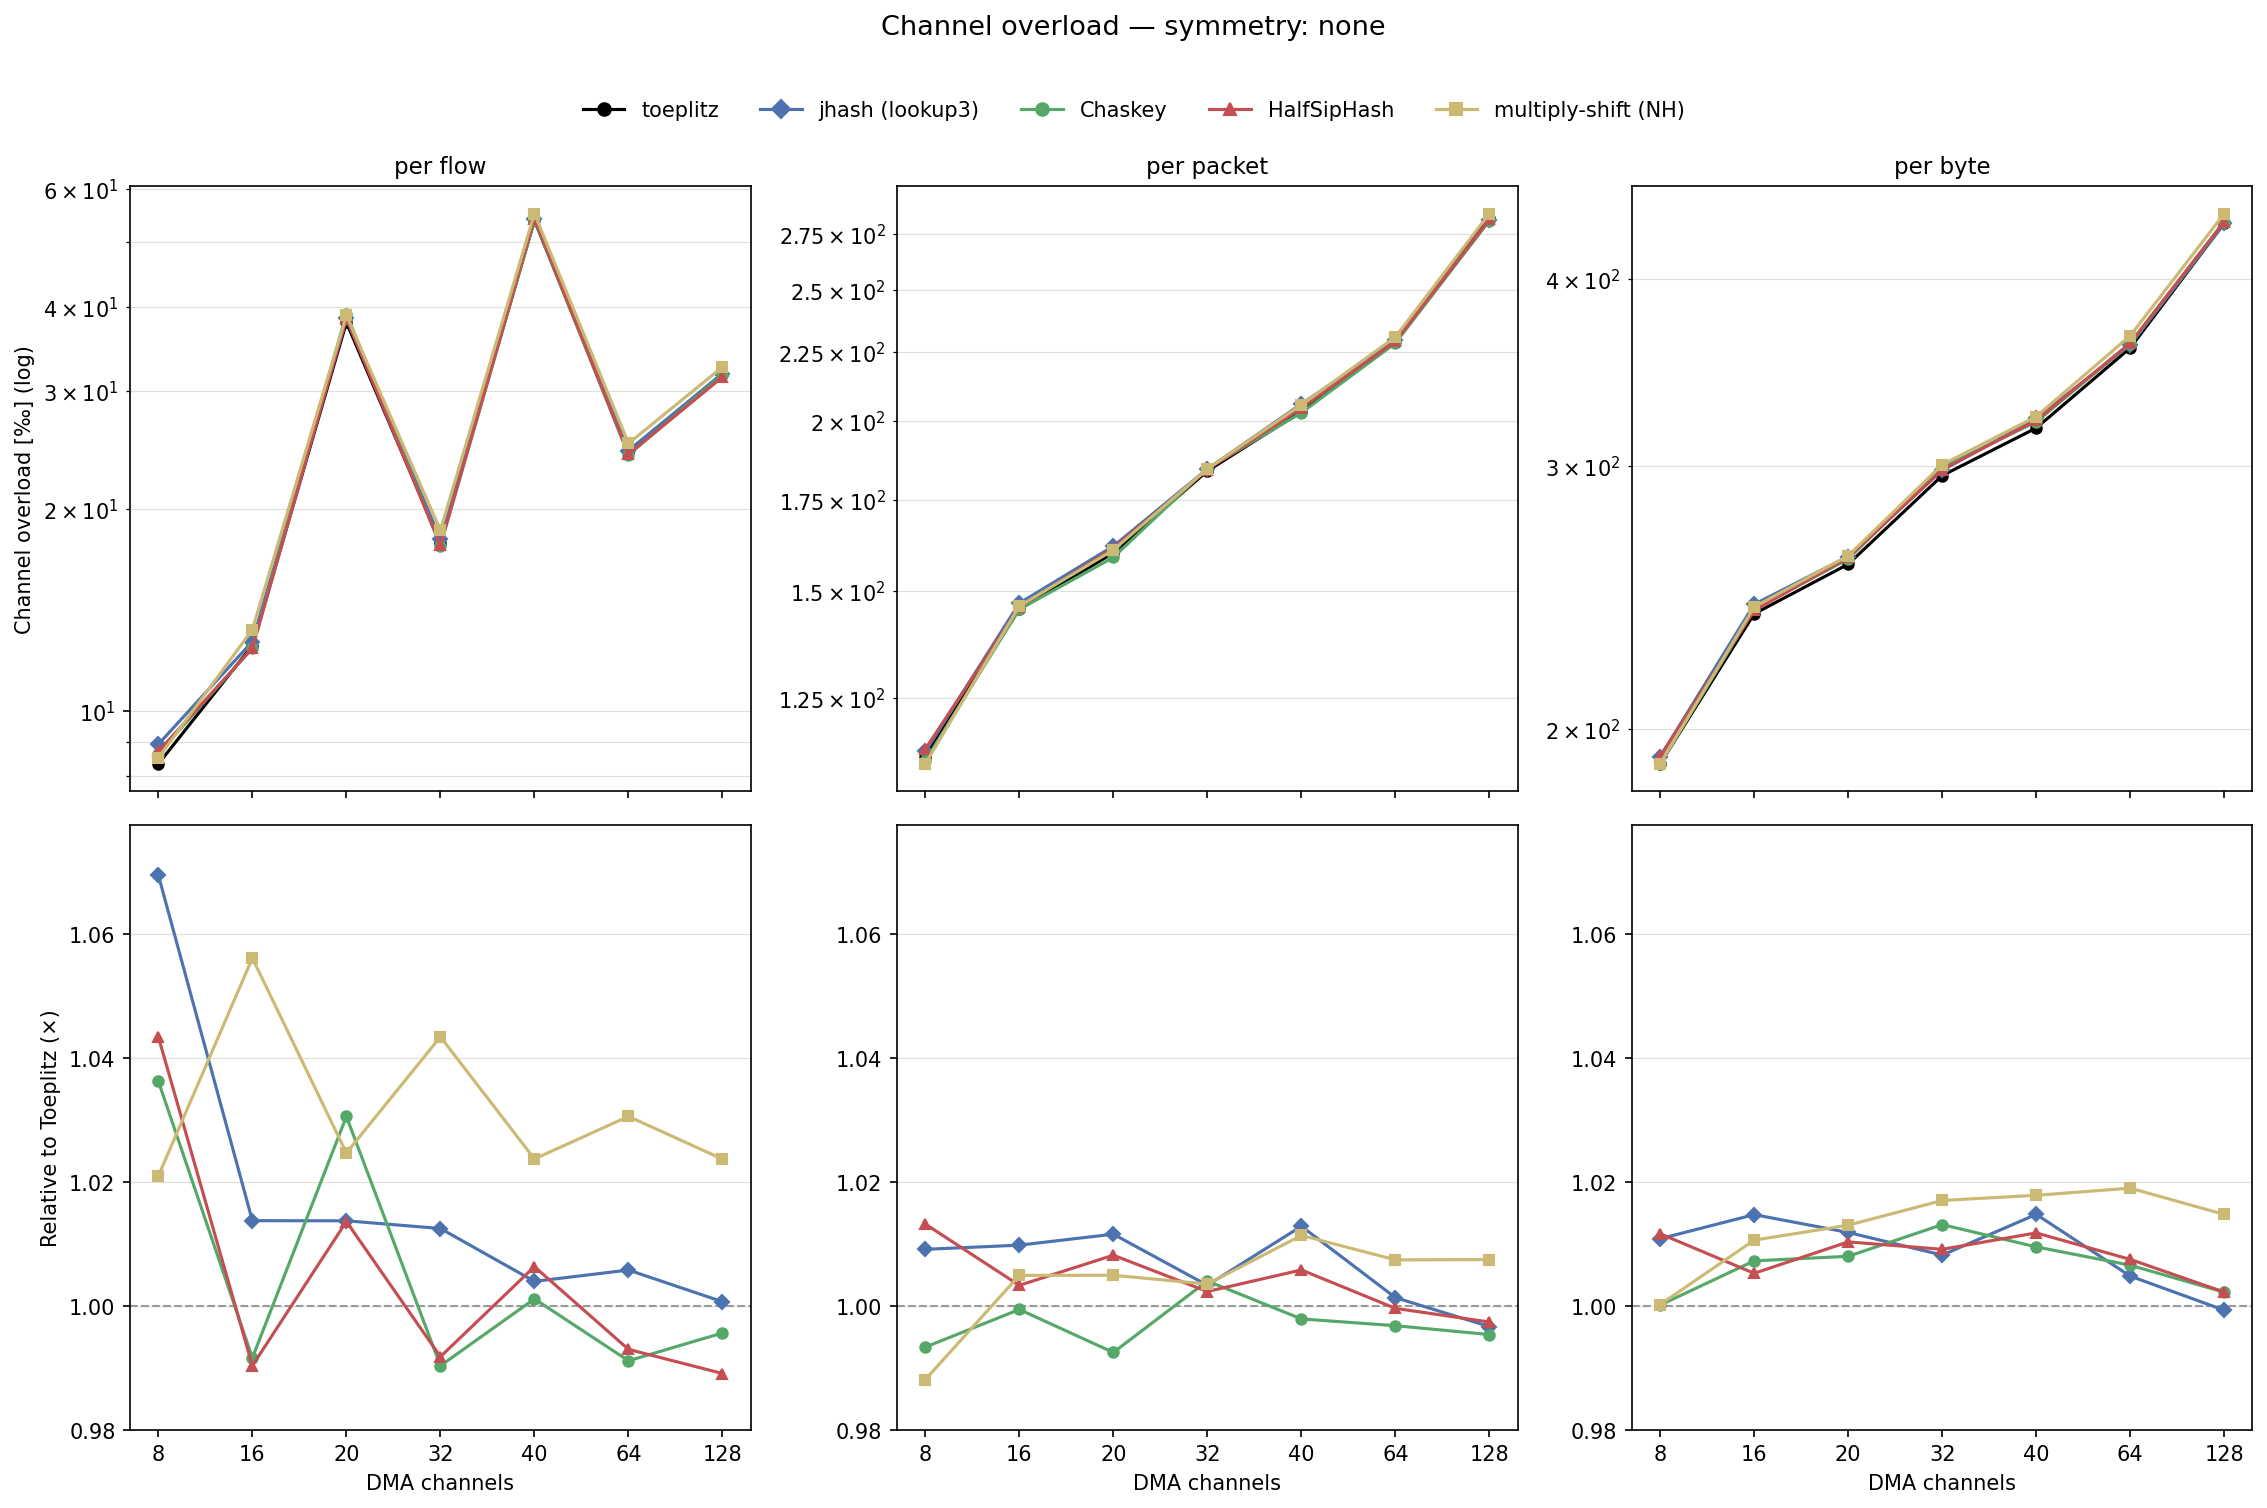
\includegraphics[width=\textwidth]{ostatne_vzorky/odid6_full_tuple/overload_none.png}
    \caption{bez symetrie}
  \end{subfigure}

  \begin{subfigure}{0.60\textwidth}
    \centering
    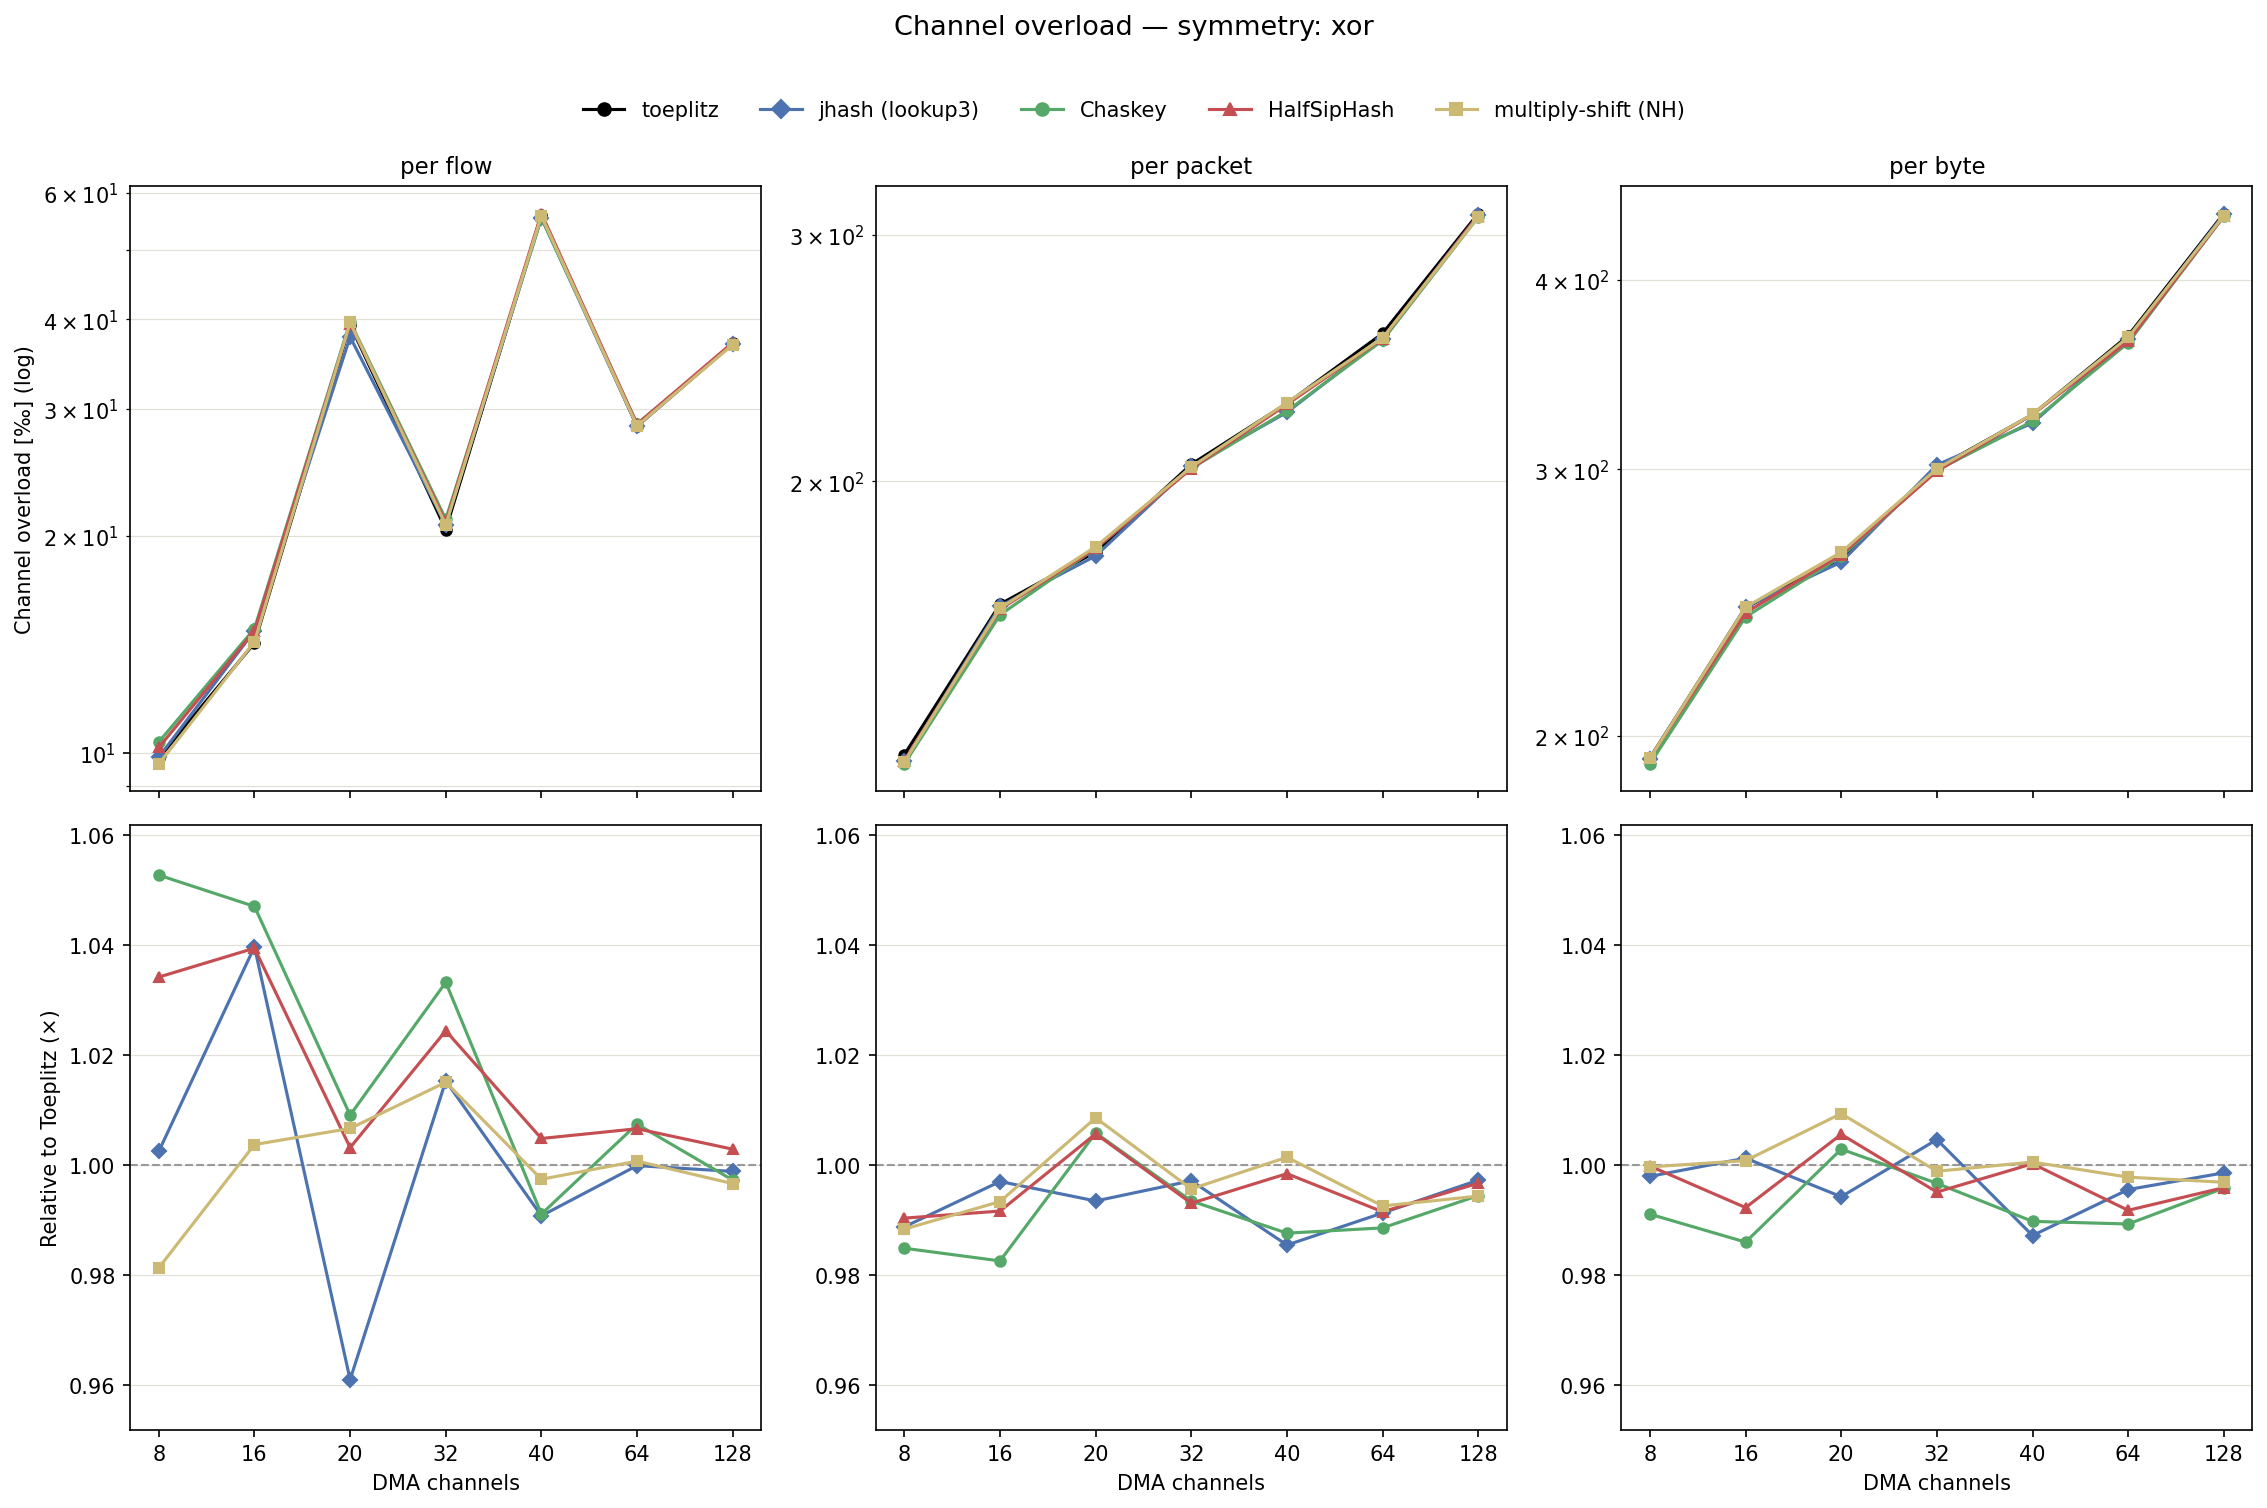
\includegraphics[width=\textwidth]{ostatne_vzorky/odid6_full_tuple/overload_xorfold.png}
    \caption{symetria XOR}
  \end{subfigure}

  \begin{subfigure}{0.60\textwidth}
    \centering
    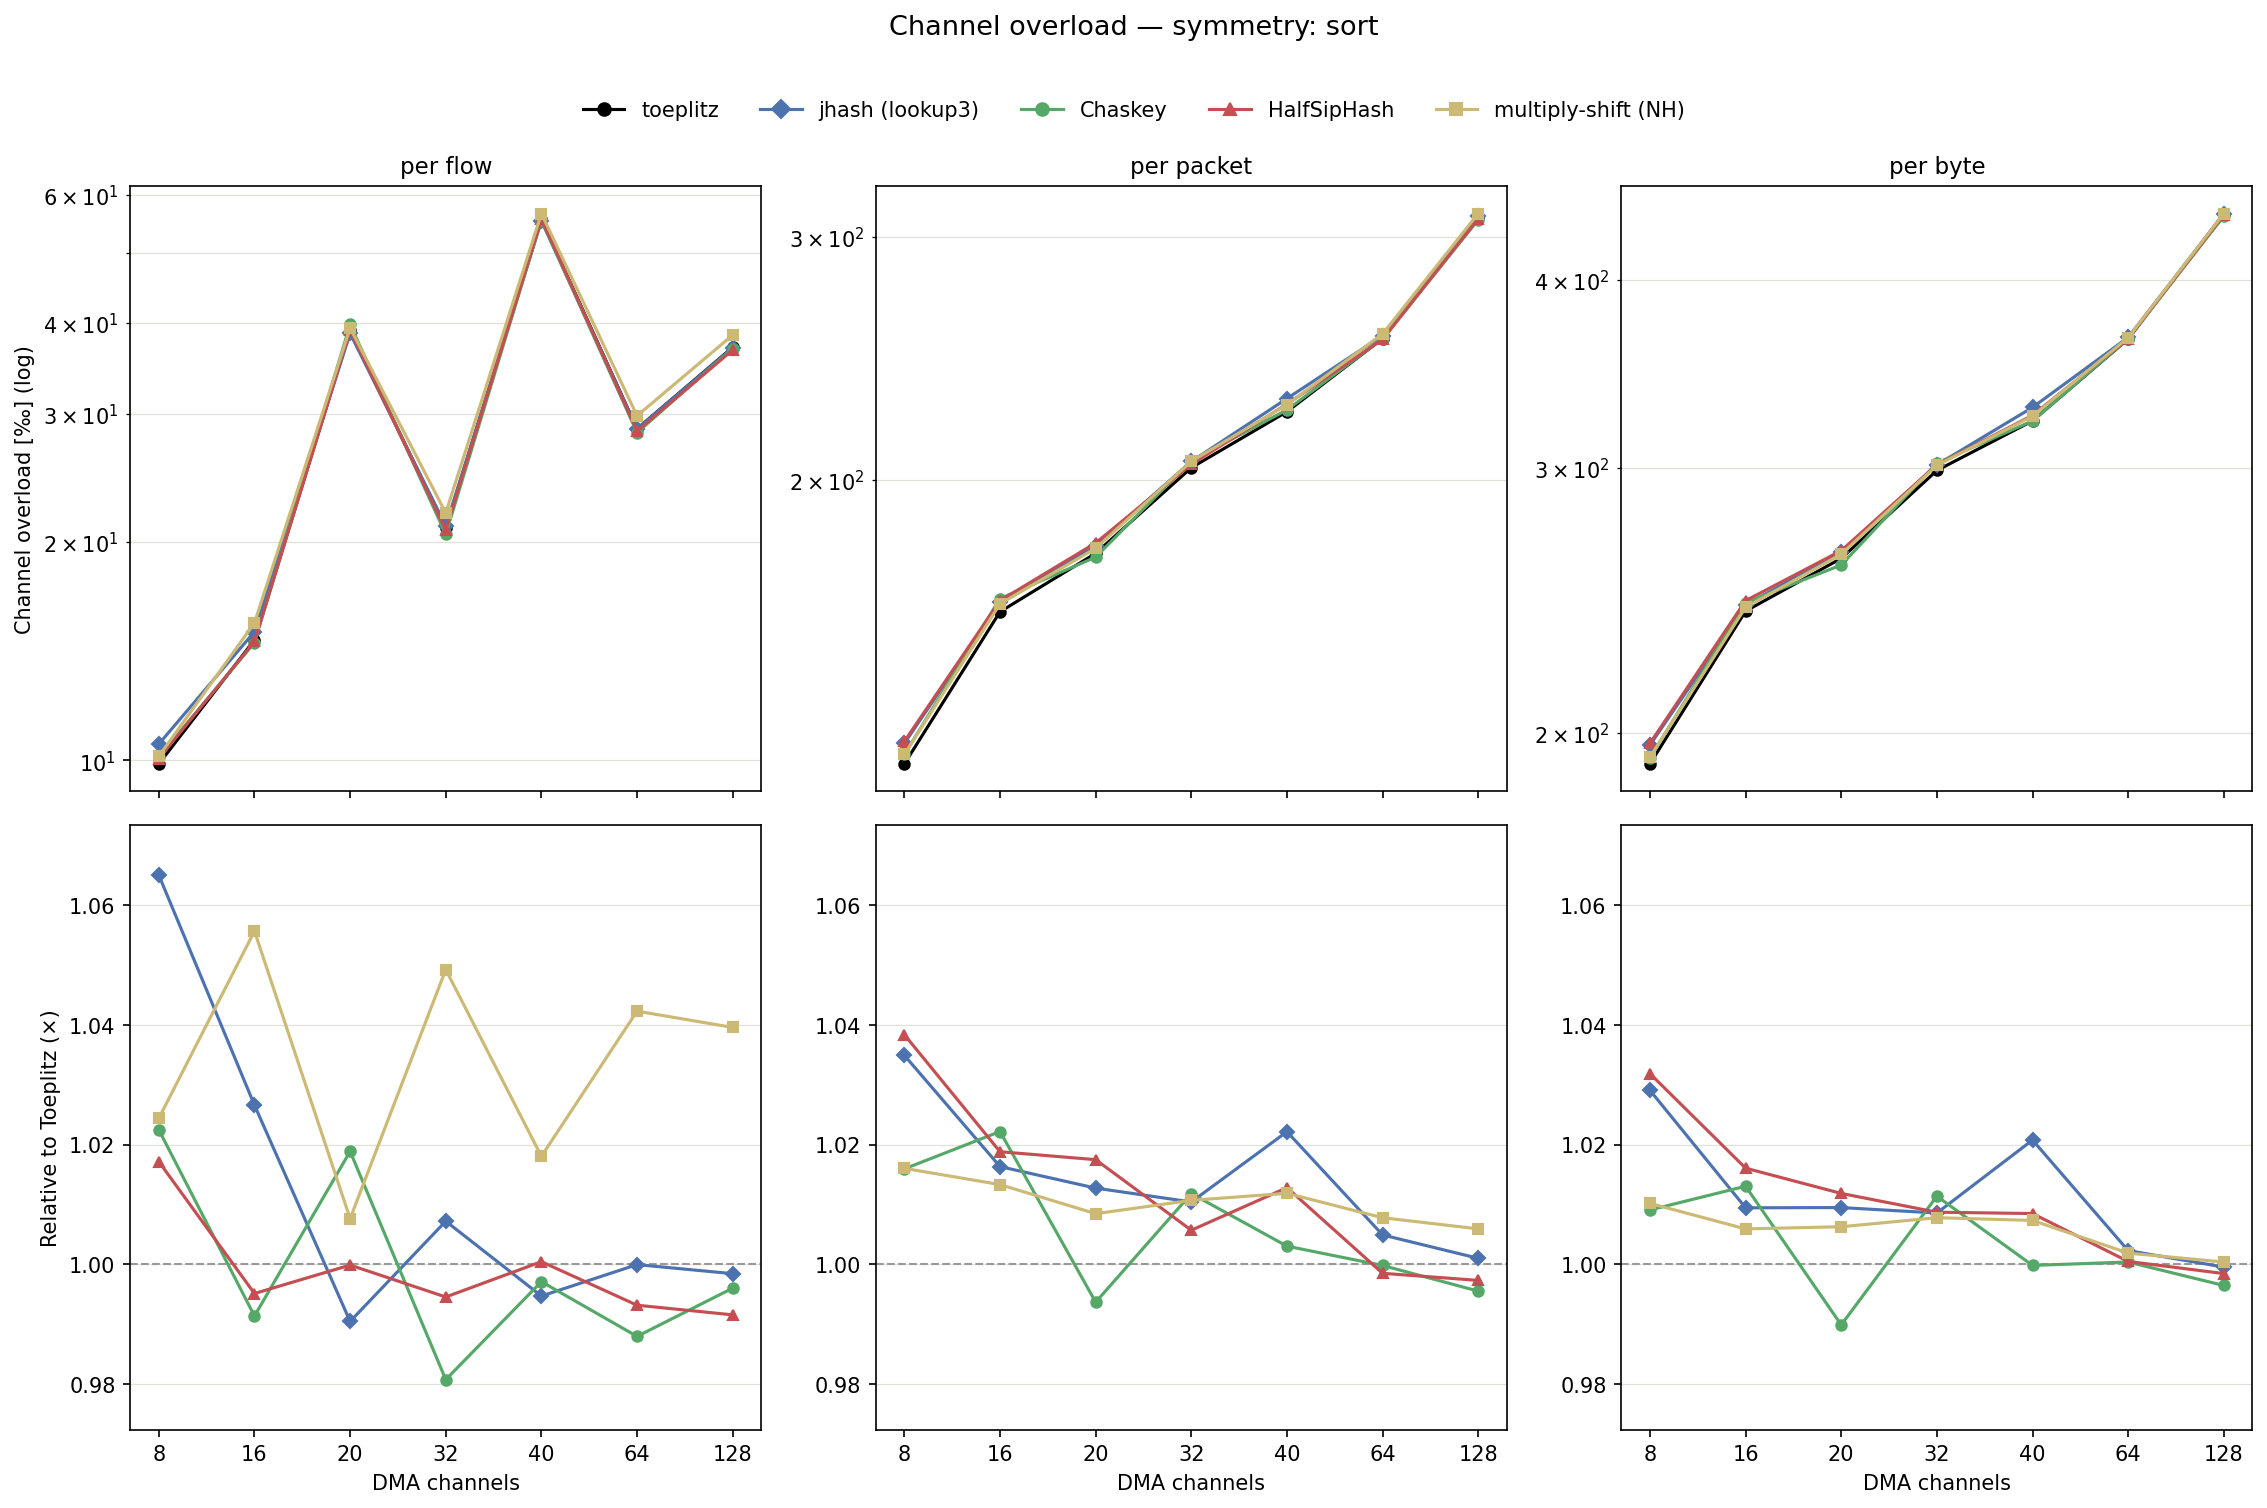
\includegraphics[width=\textwidth]{ostatne_vzorky/odid6_full_tuple/overload_sortfold.png}
    \caption{symetria sort}
  \end{subfigure}

  \caption{Preťaženie funkcií a pomer k~Toeplitzu: \texttt{odid6}, plný tuple.}
  \label{fig:b-odid6-full-tuple-overload}
\end{figure}

\begin{figure}[p]
  \centering
  \begin{subfigure}{0.54\textwidth}
    \centering
    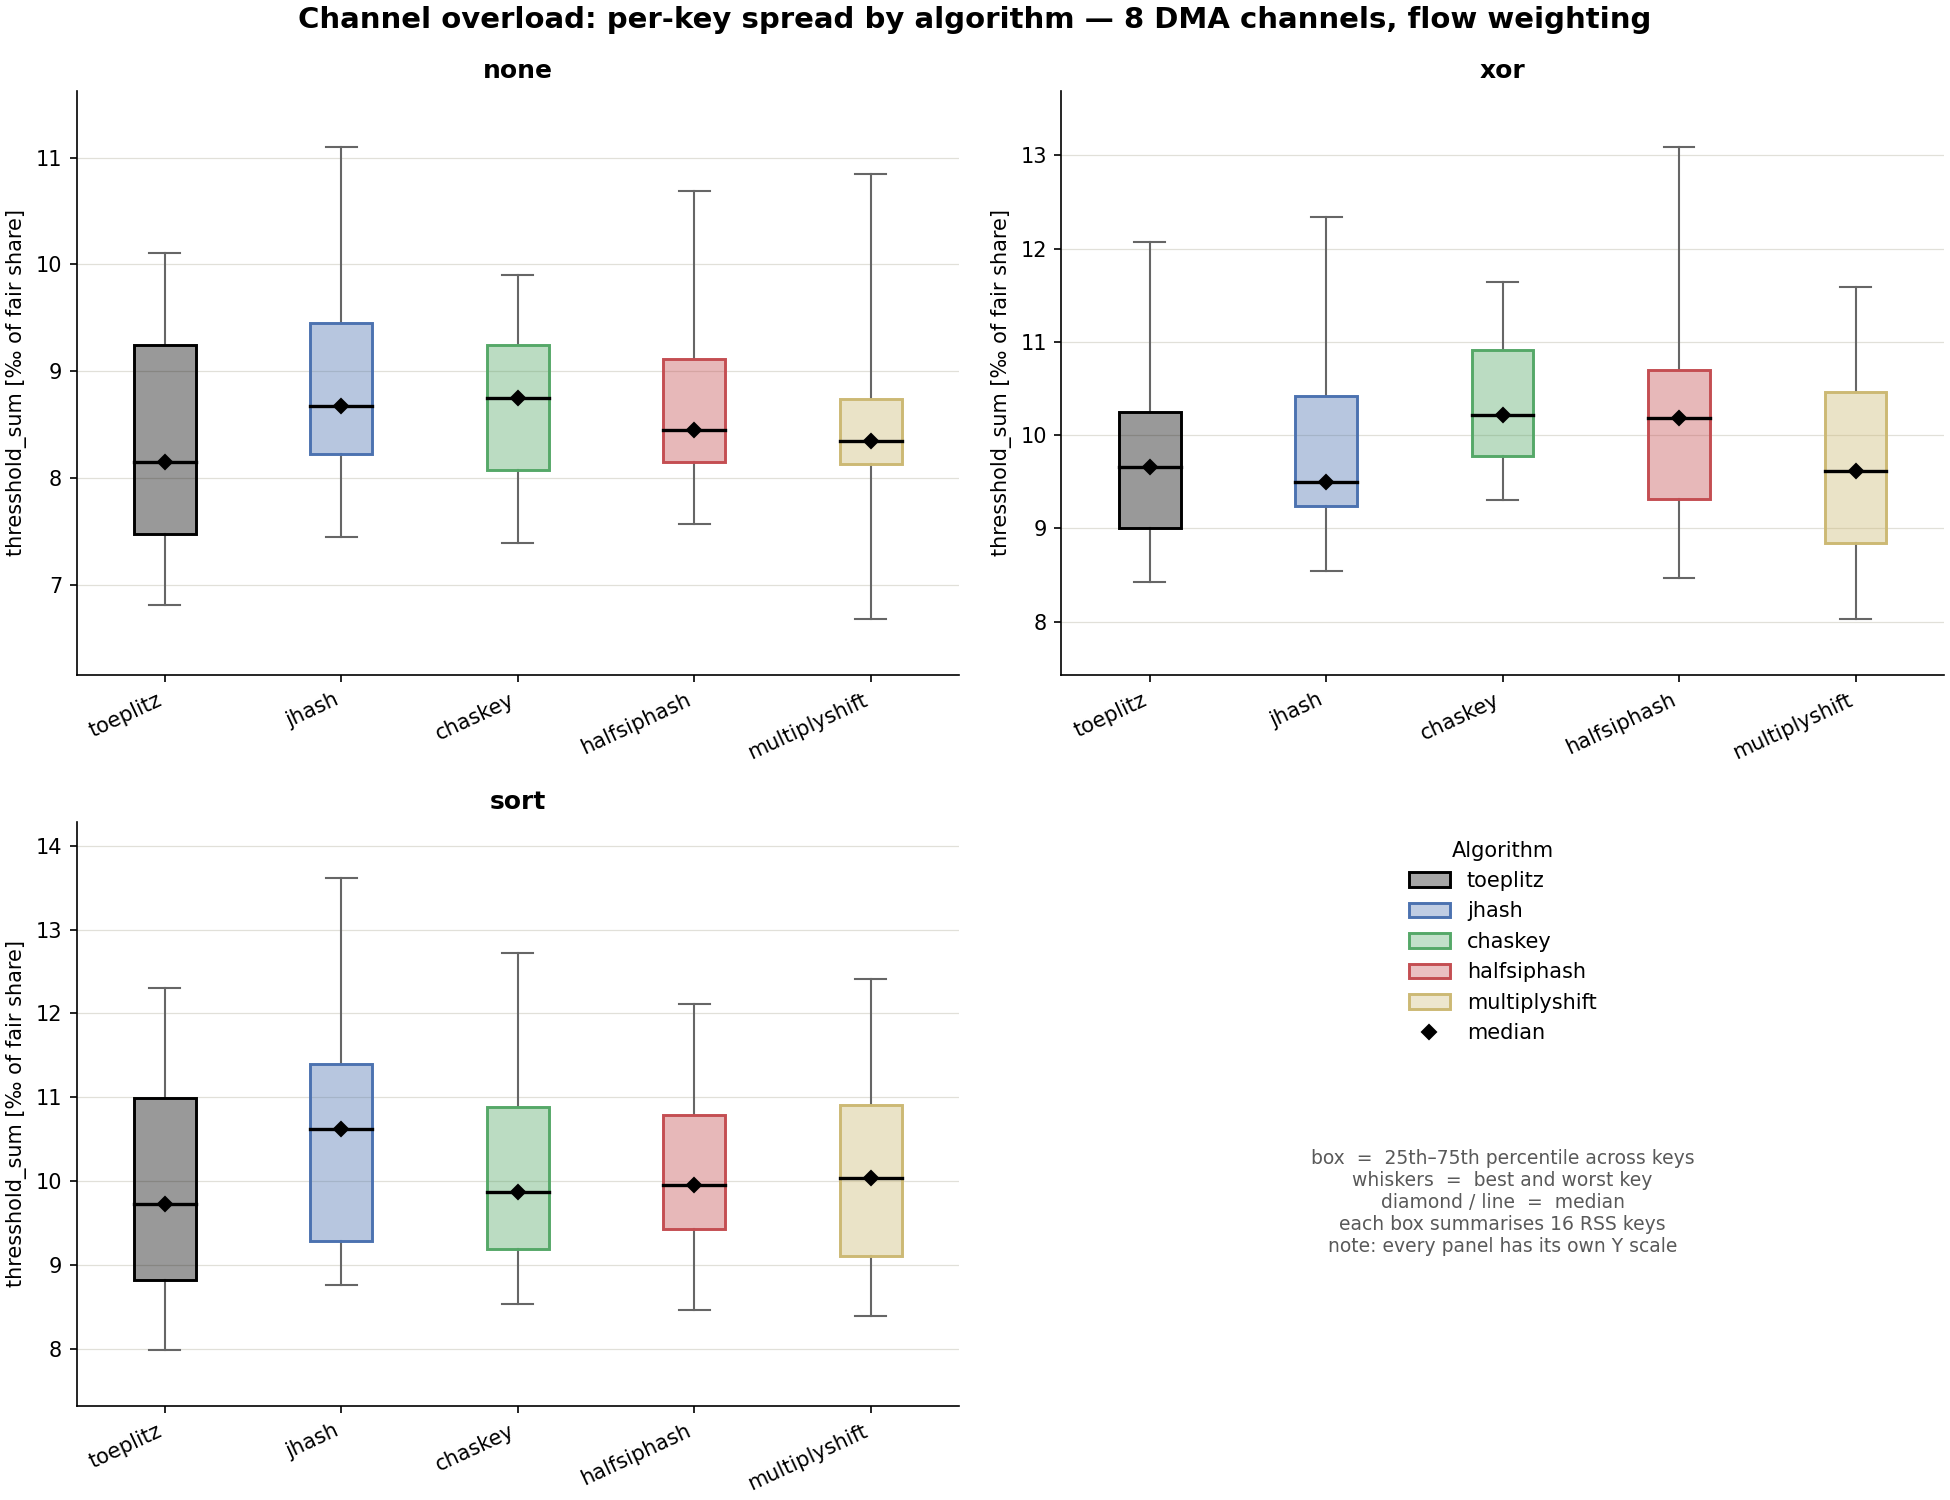
\includegraphics[width=\textwidth]{ostatne_vzorky/odid6_full_tuple/keys_8.png}
    \caption{8 kanálov}
  \end{subfigure}

  \begin{subfigure}{0.54\textwidth}
    \centering
    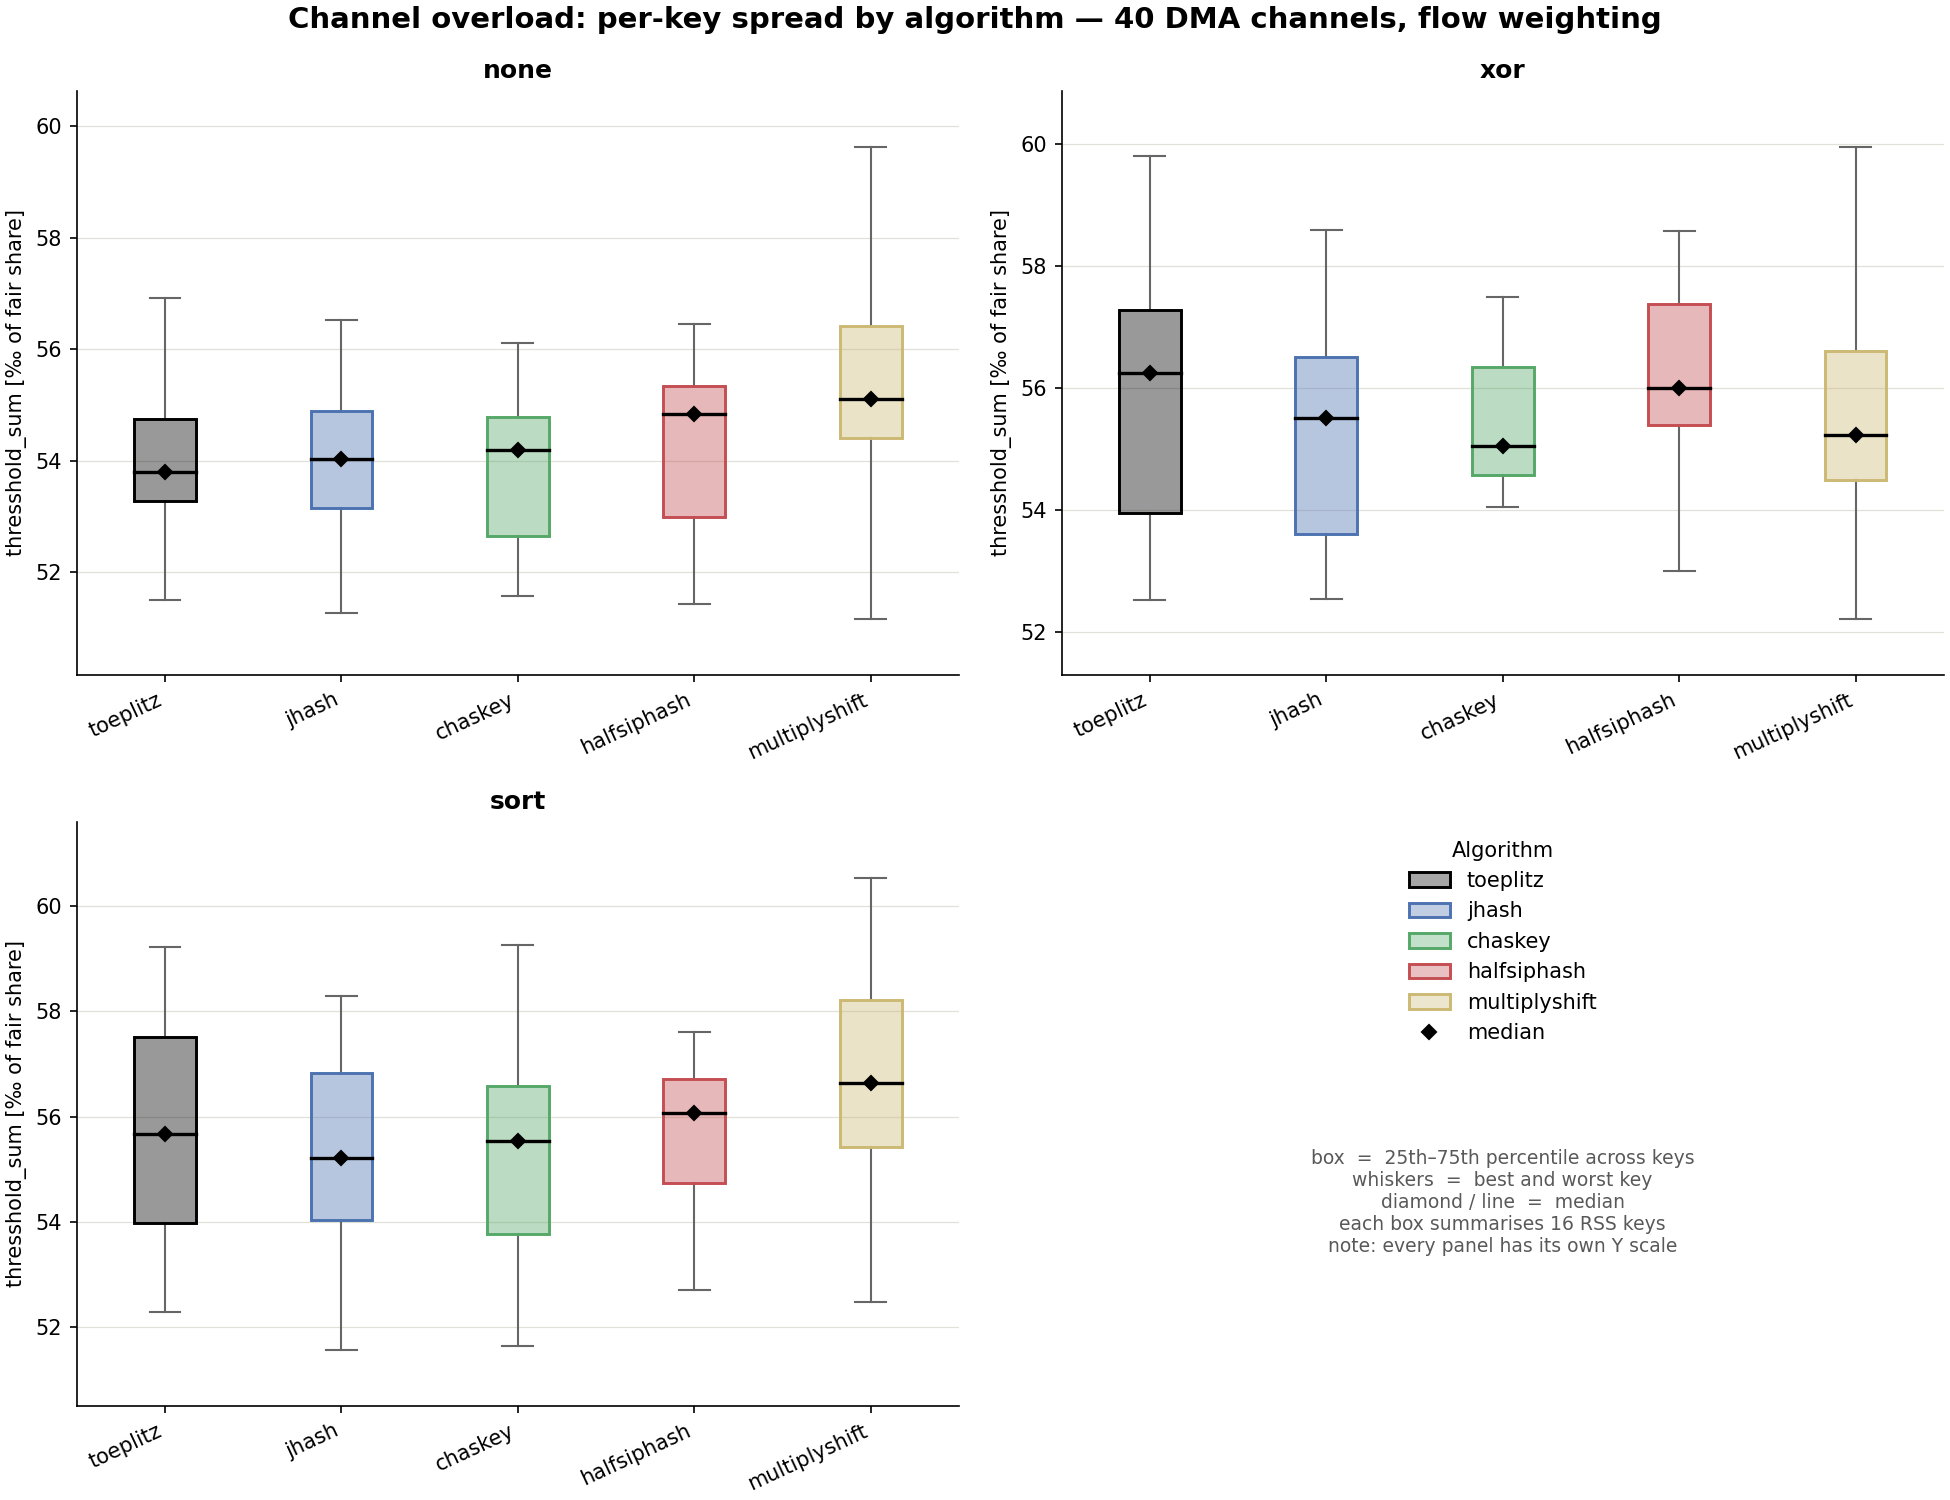
\includegraphics[width=\textwidth]{ostatne_vzorky/odid6_full_tuple/keys_40.png}
    \caption{40 kanálov}
  \end{subfigure}

  \begin{subfigure}{0.54\textwidth}
    \centering
    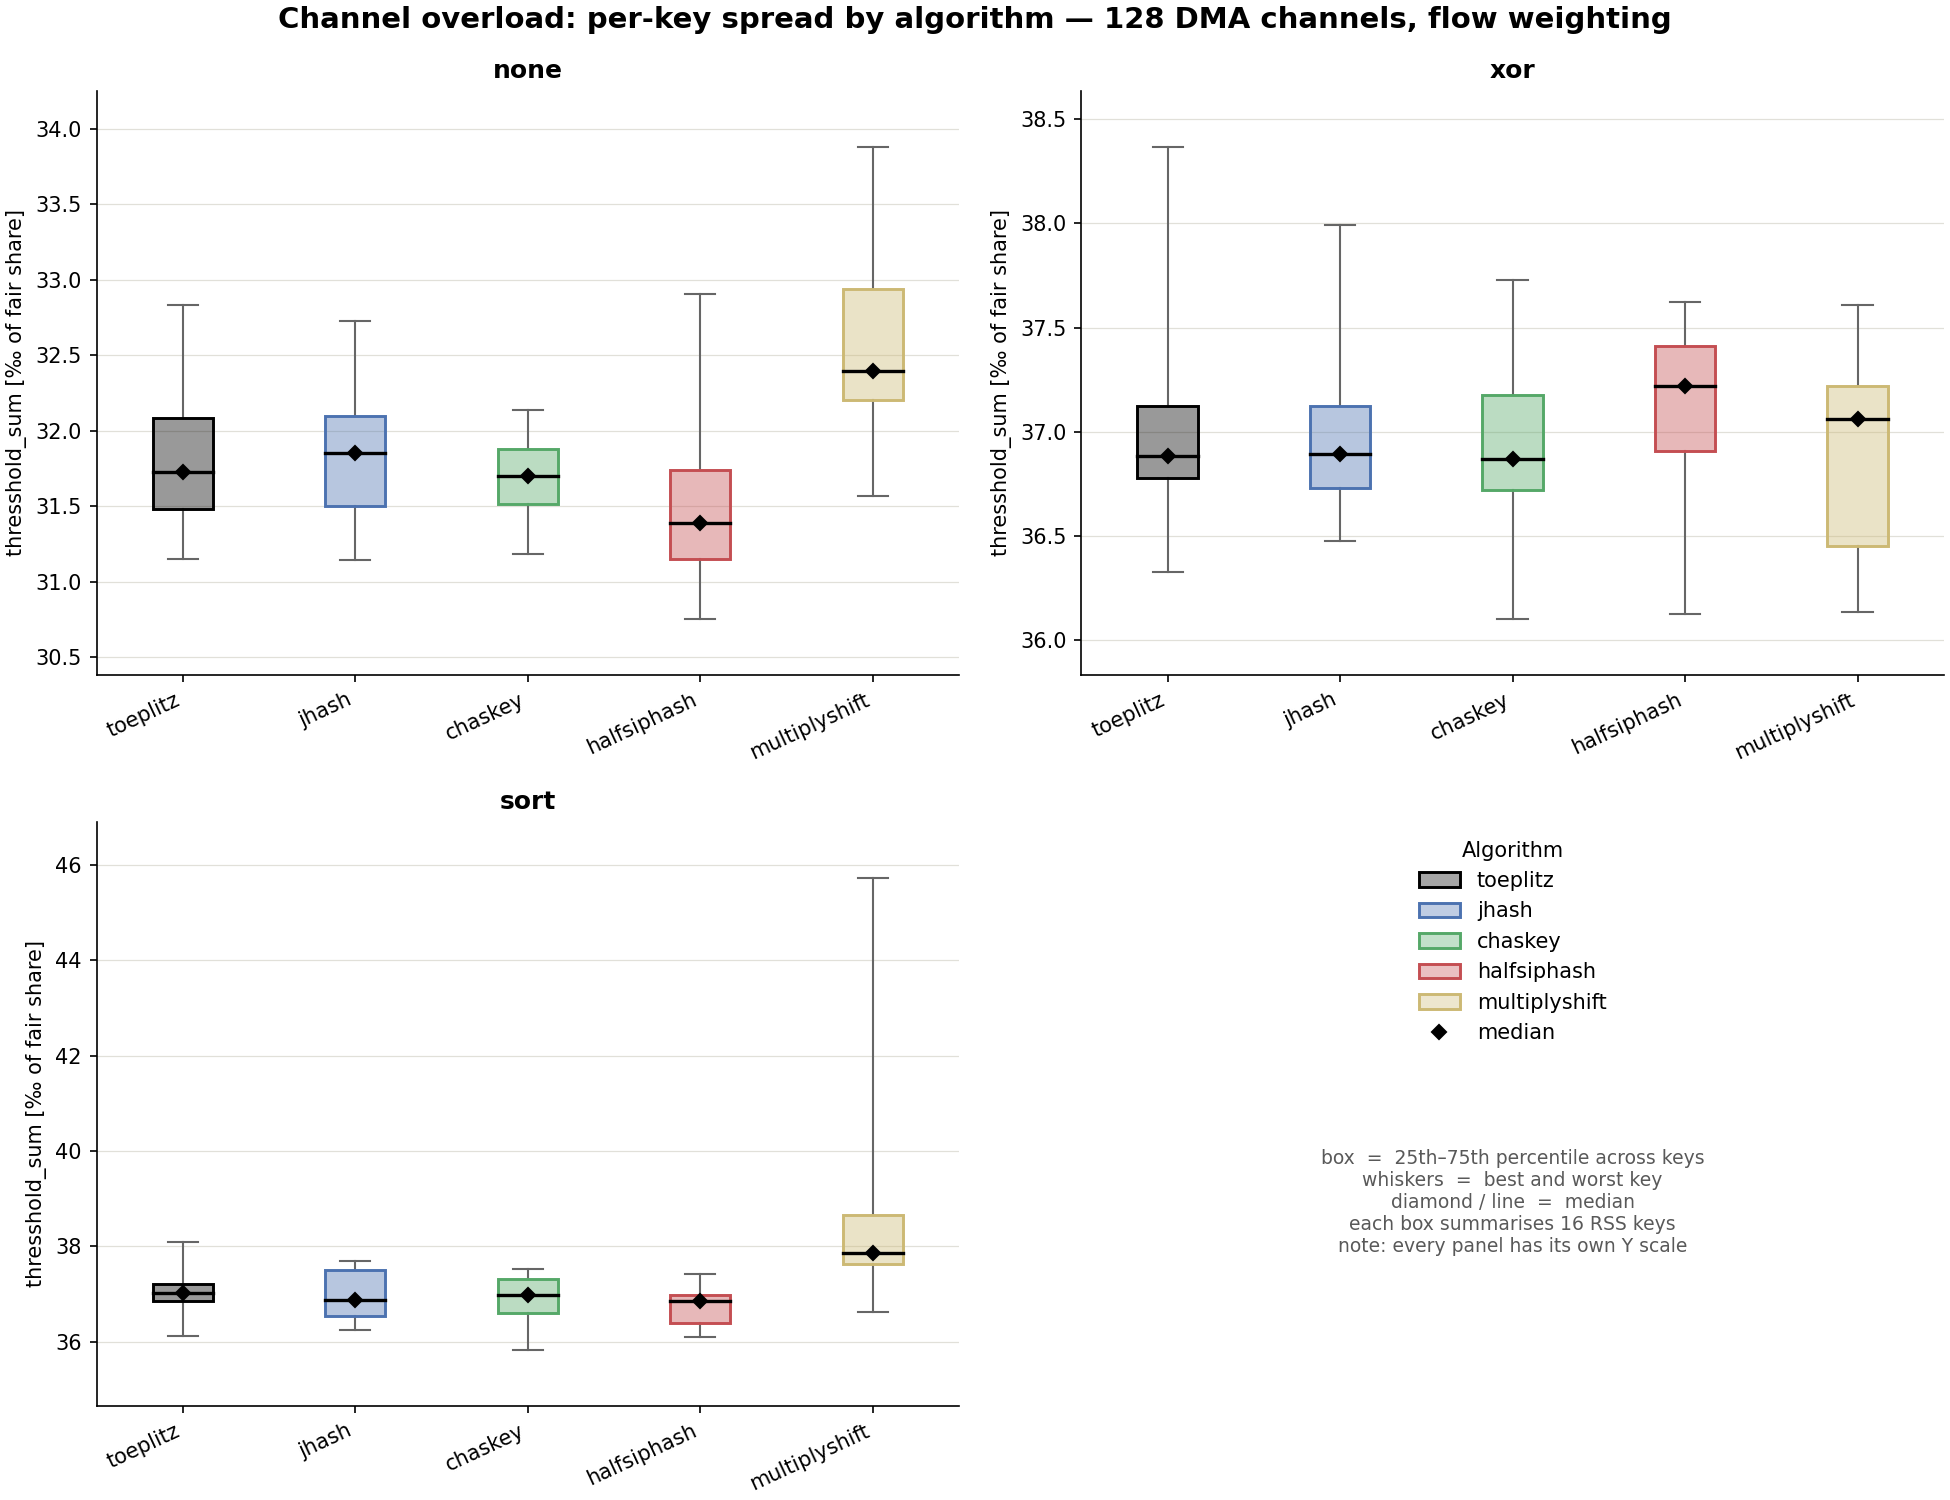
\includegraphics[width=\textwidth]{ostatne_vzorky/odid6_full_tuple/keys_128.png}
    \caption{128 kanálov}
  \end{subfigure}

  \caption{Rozptyl preťaženia medzi 16 kľúčmi pri váhe \texttt{flow}: \texttt{odid6}, plný tuple.}
  \label{fig:b-odid6-full-tuple-keys}
\end{figure}

\begin{figure}[ht]
  \centering
  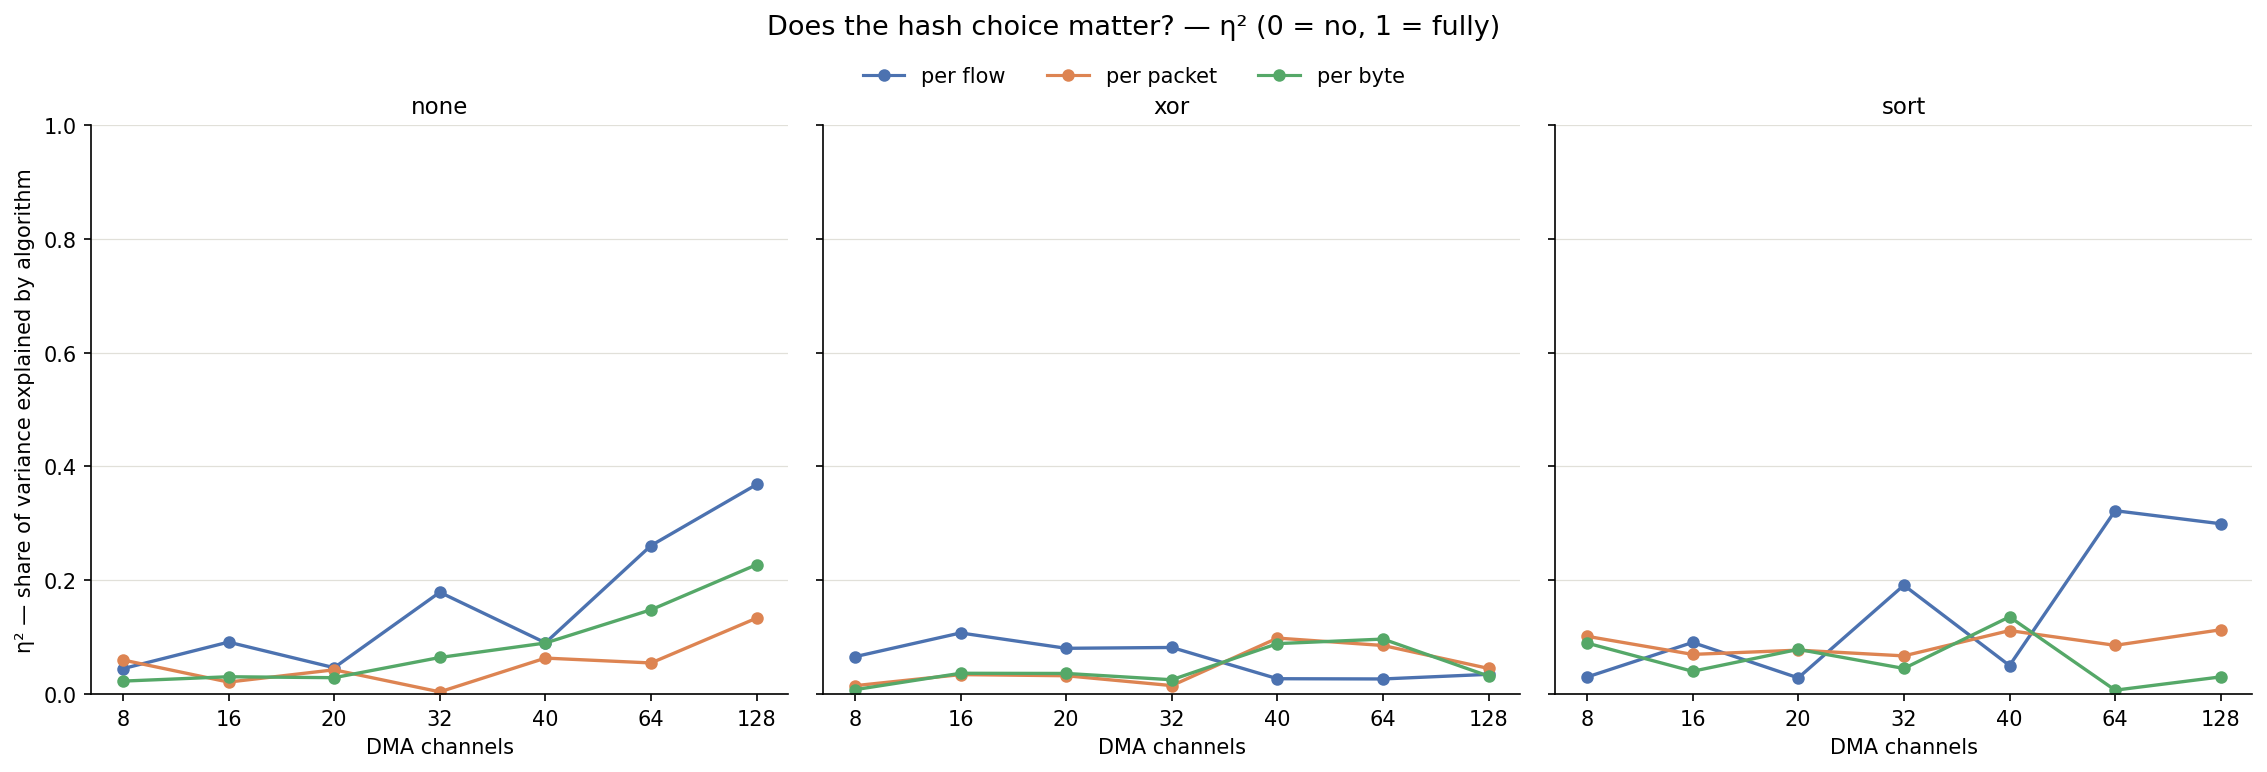
\includegraphics[width=0.9\textwidth]{ostatne_vzorky/odid6_full_tuple/spread.png}
  \caption{Podiel rozptylu vysvetlený voľbou funkcie ($\eta^2$): \texttt{odid6}, plný tuple.}
  \label{fig:b-odid6-full-tuple-spread}
\end{figure}

\clearpage
\begin{figure}[p]
  \centering
  \begin{subfigure}{0.60\textwidth}
    \centering
    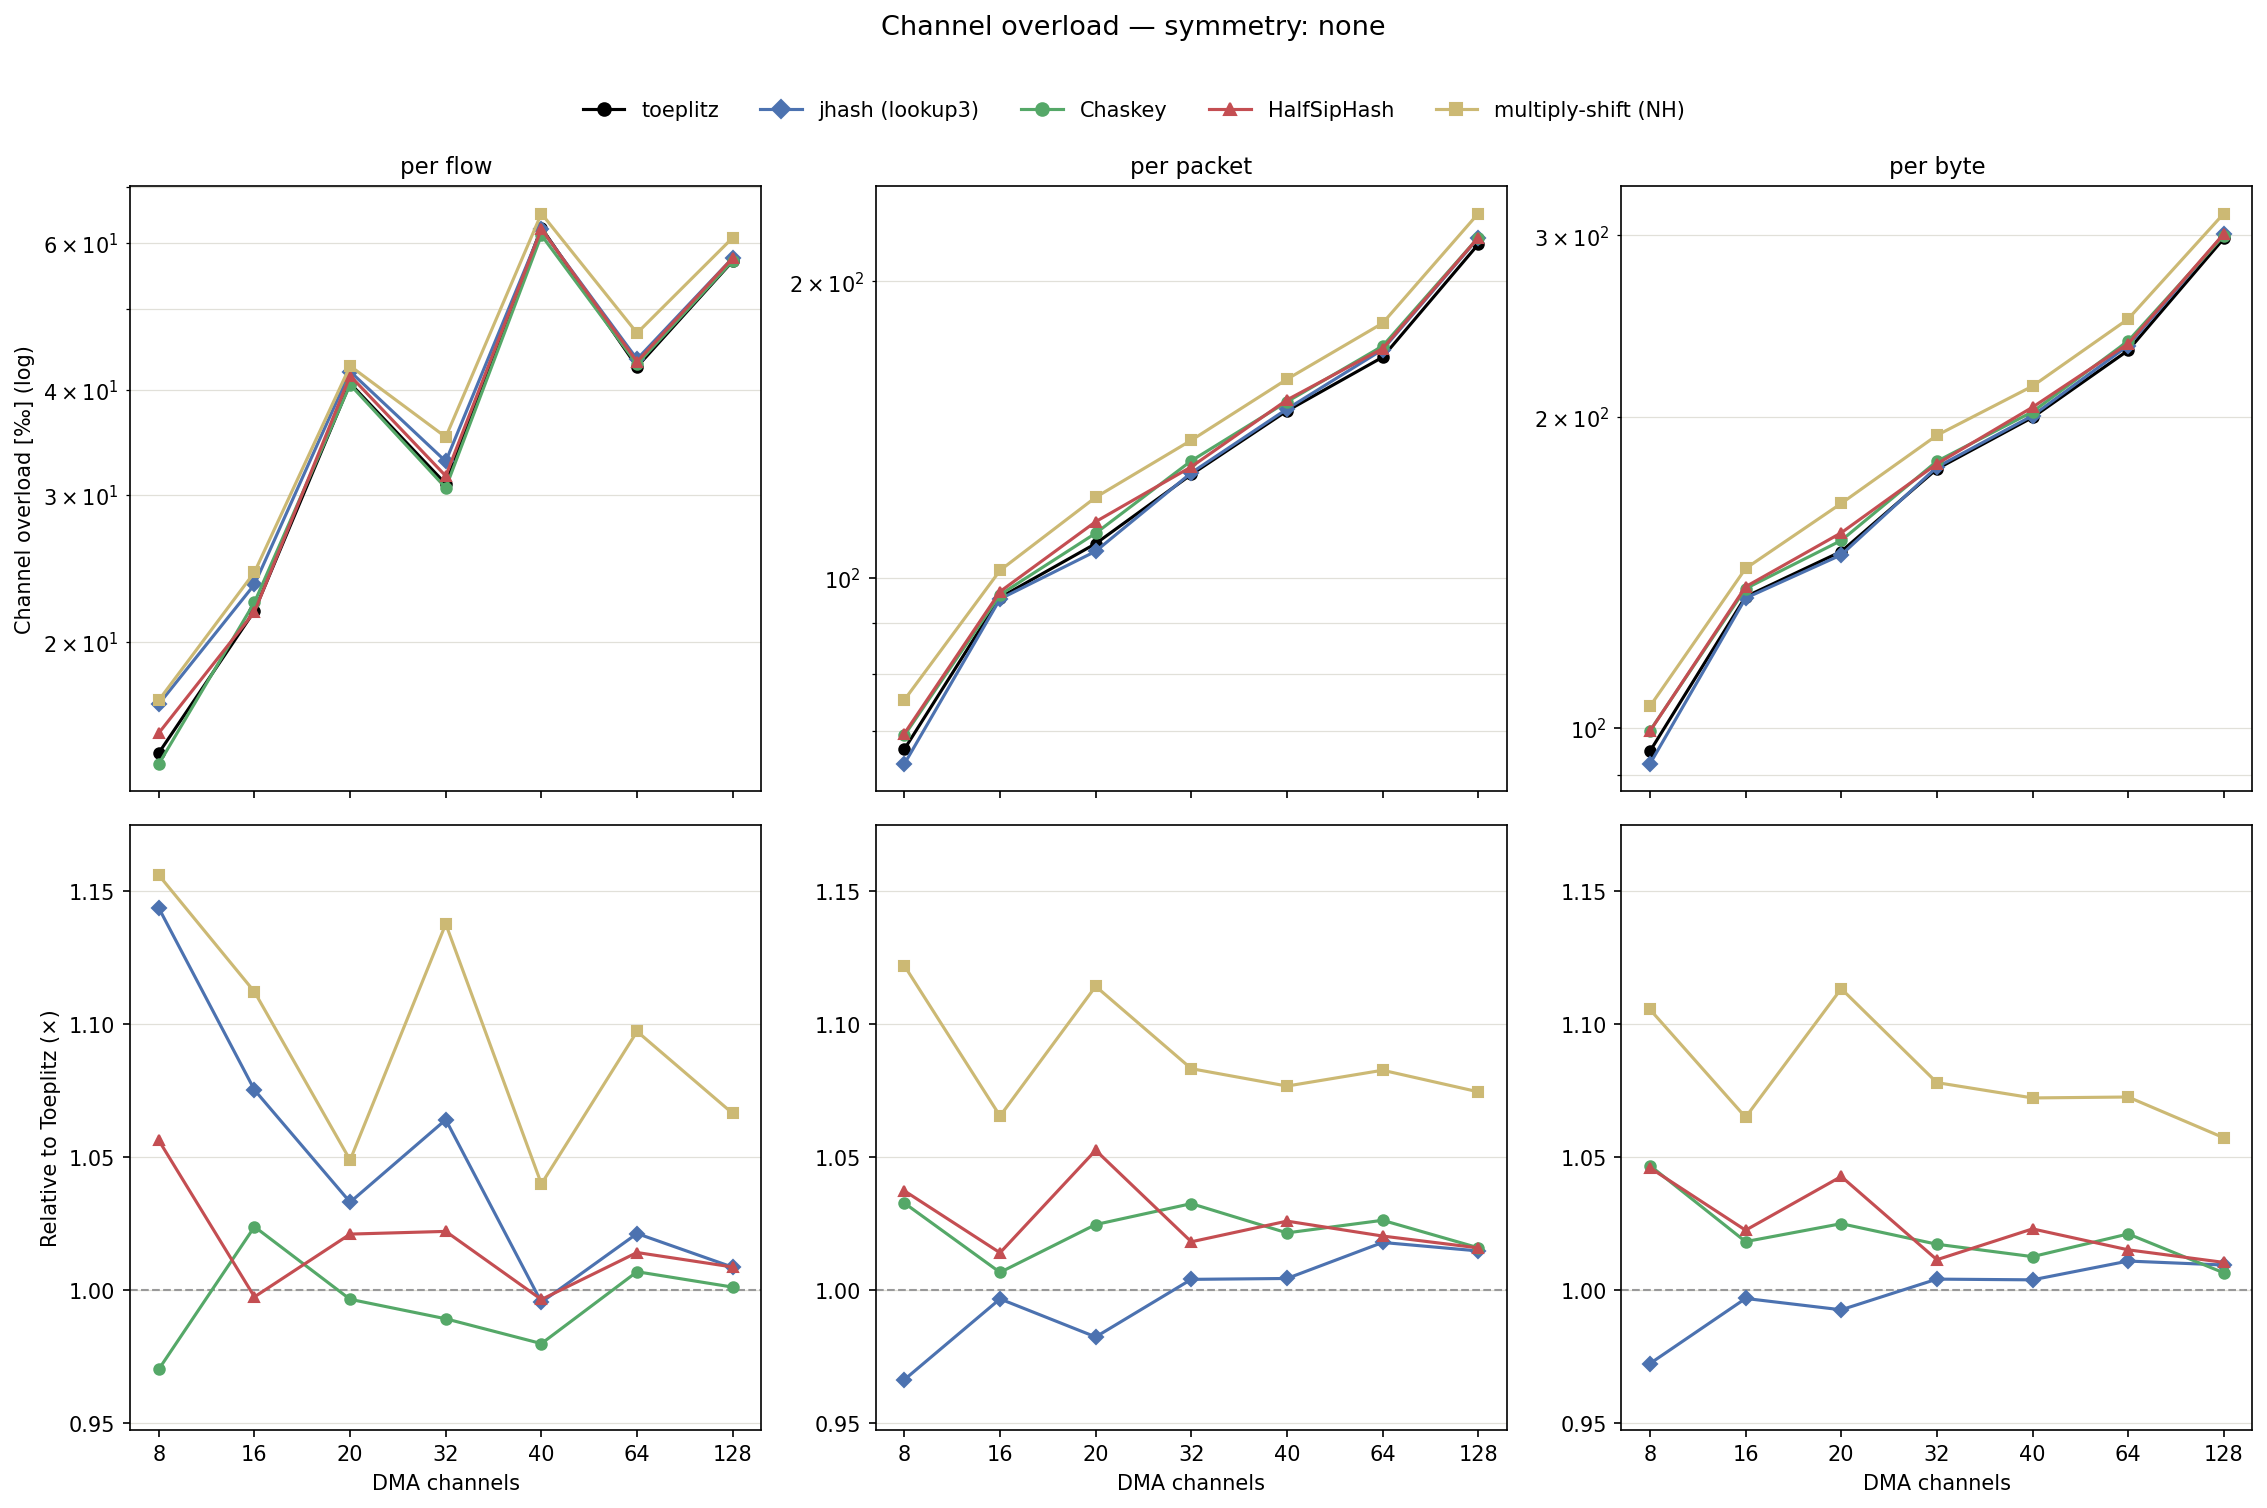
\includegraphics[width=\textwidth]{ostatne_vzorky/odid1_ip_only/overload_none.png}
    \caption{bez symetrie}
  \end{subfigure}

  \begin{subfigure}{0.60\textwidth}
    \centering
    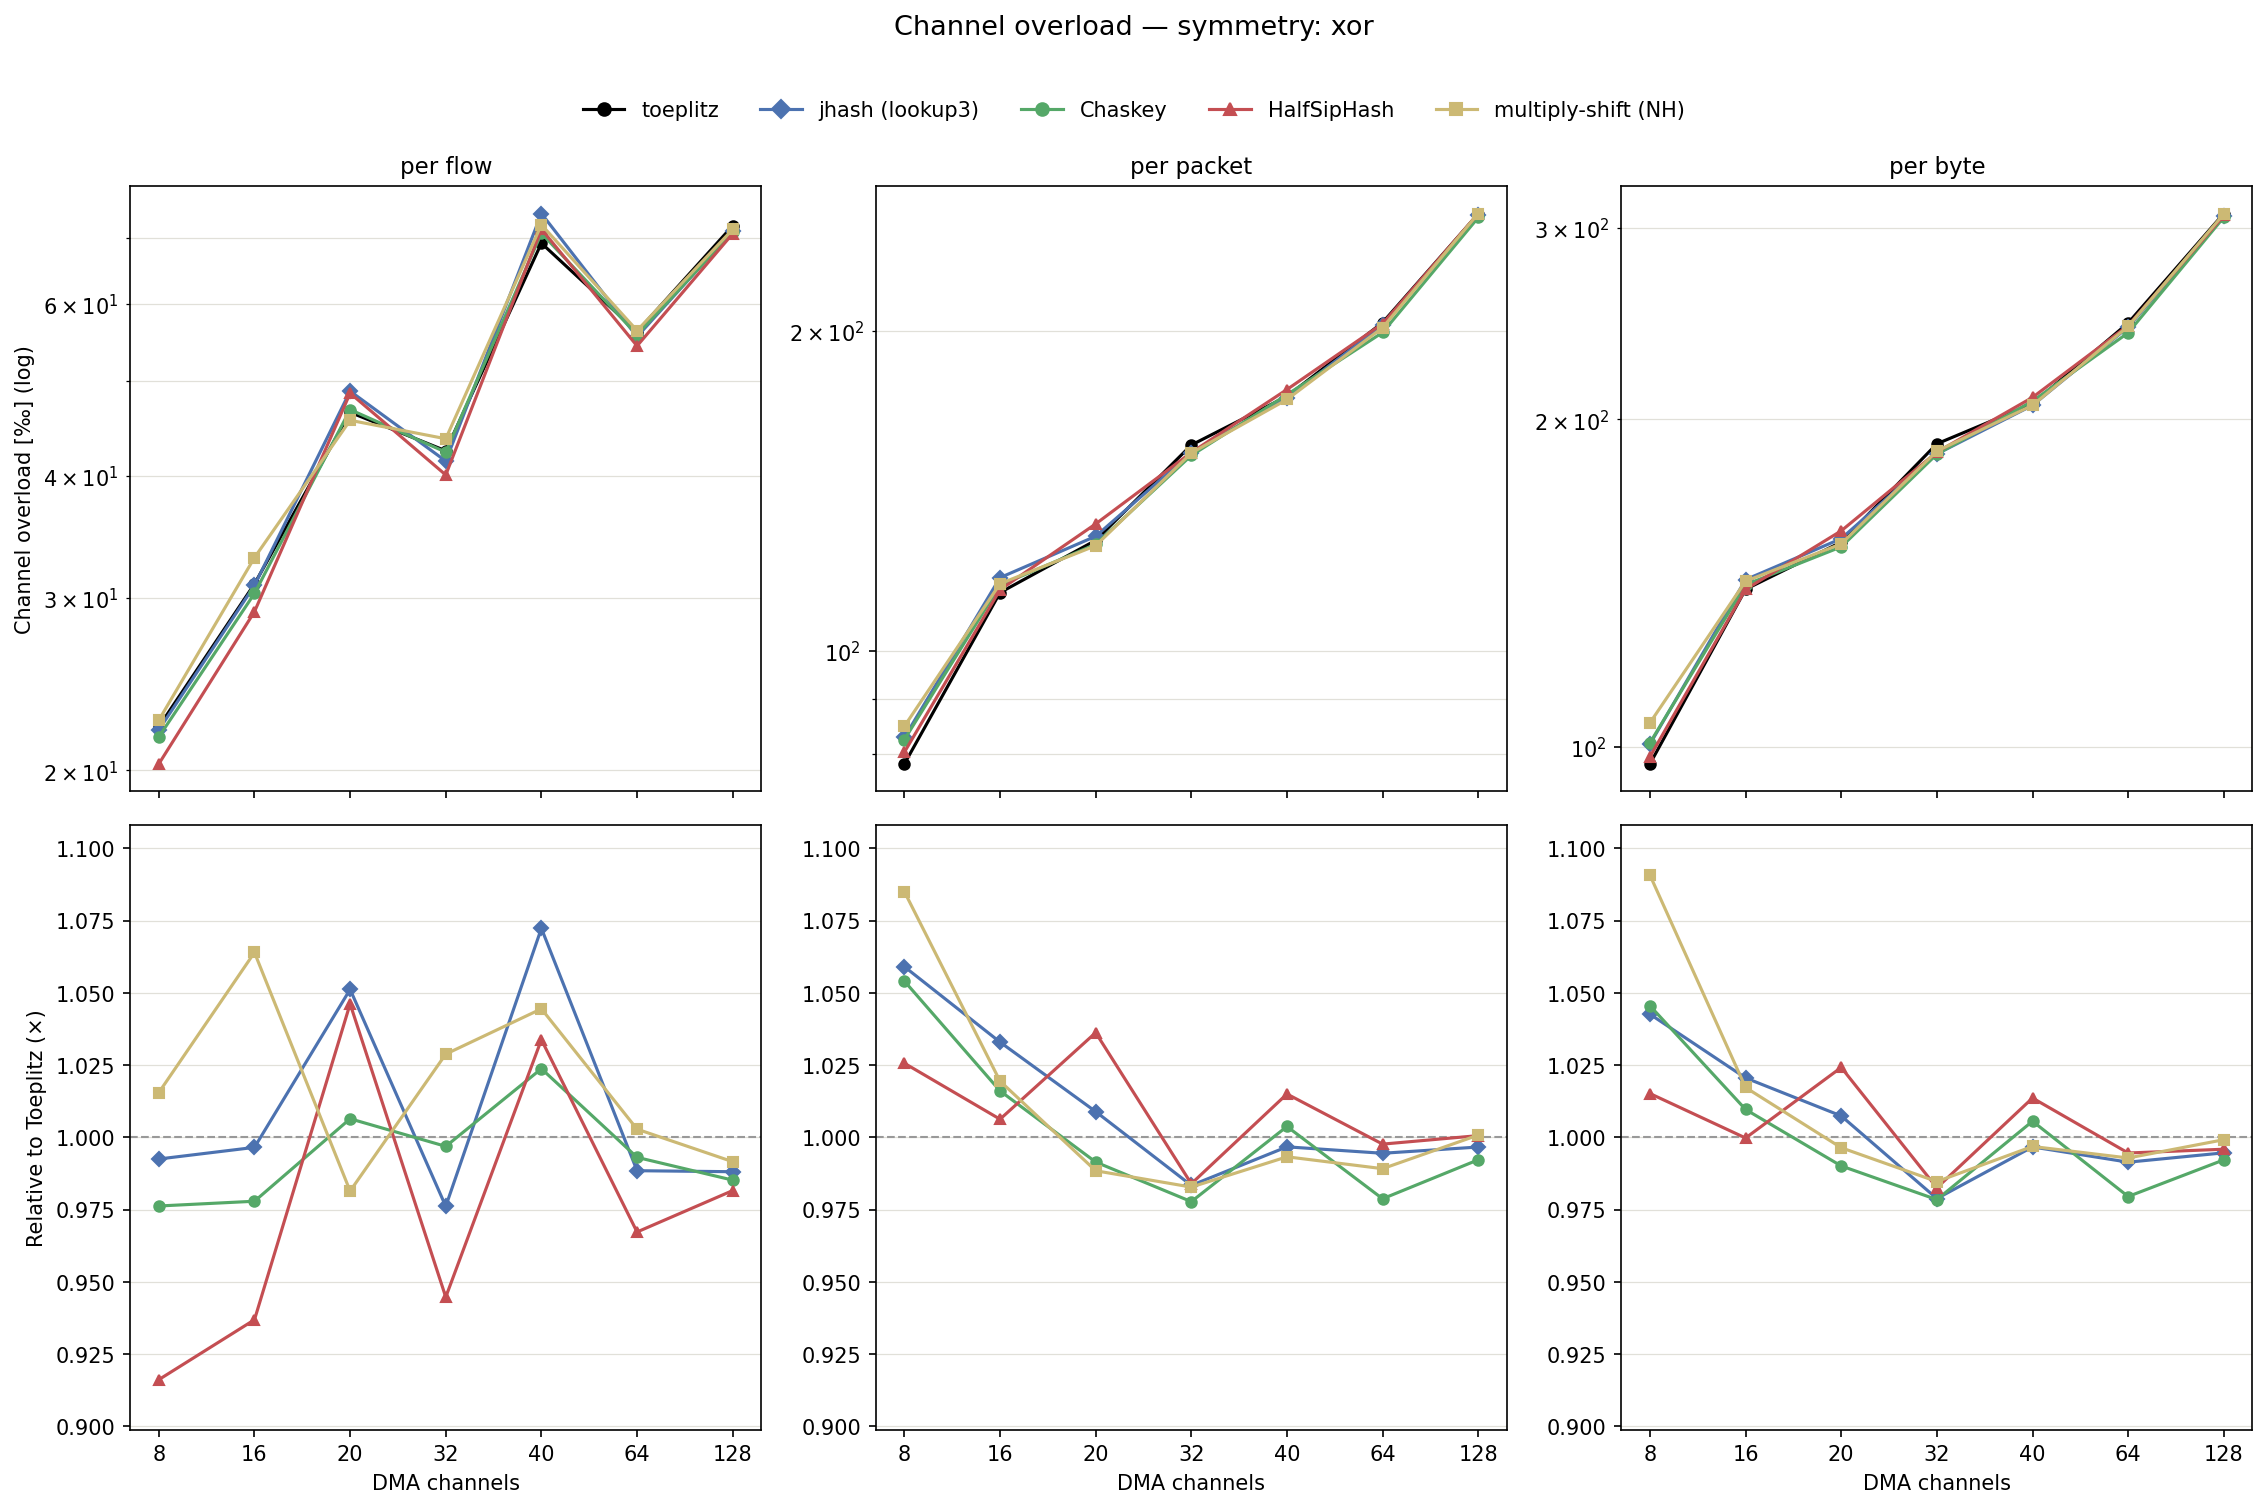
\includegraphics[width=\textwidth]{ostatne_vzorky/odid1_ip_only/overload_xorfold.png}
    \caption{symetria XOR}
  \end{subfigure}

  \begin{subfigure}{0.60\textwidth}
    \centering
    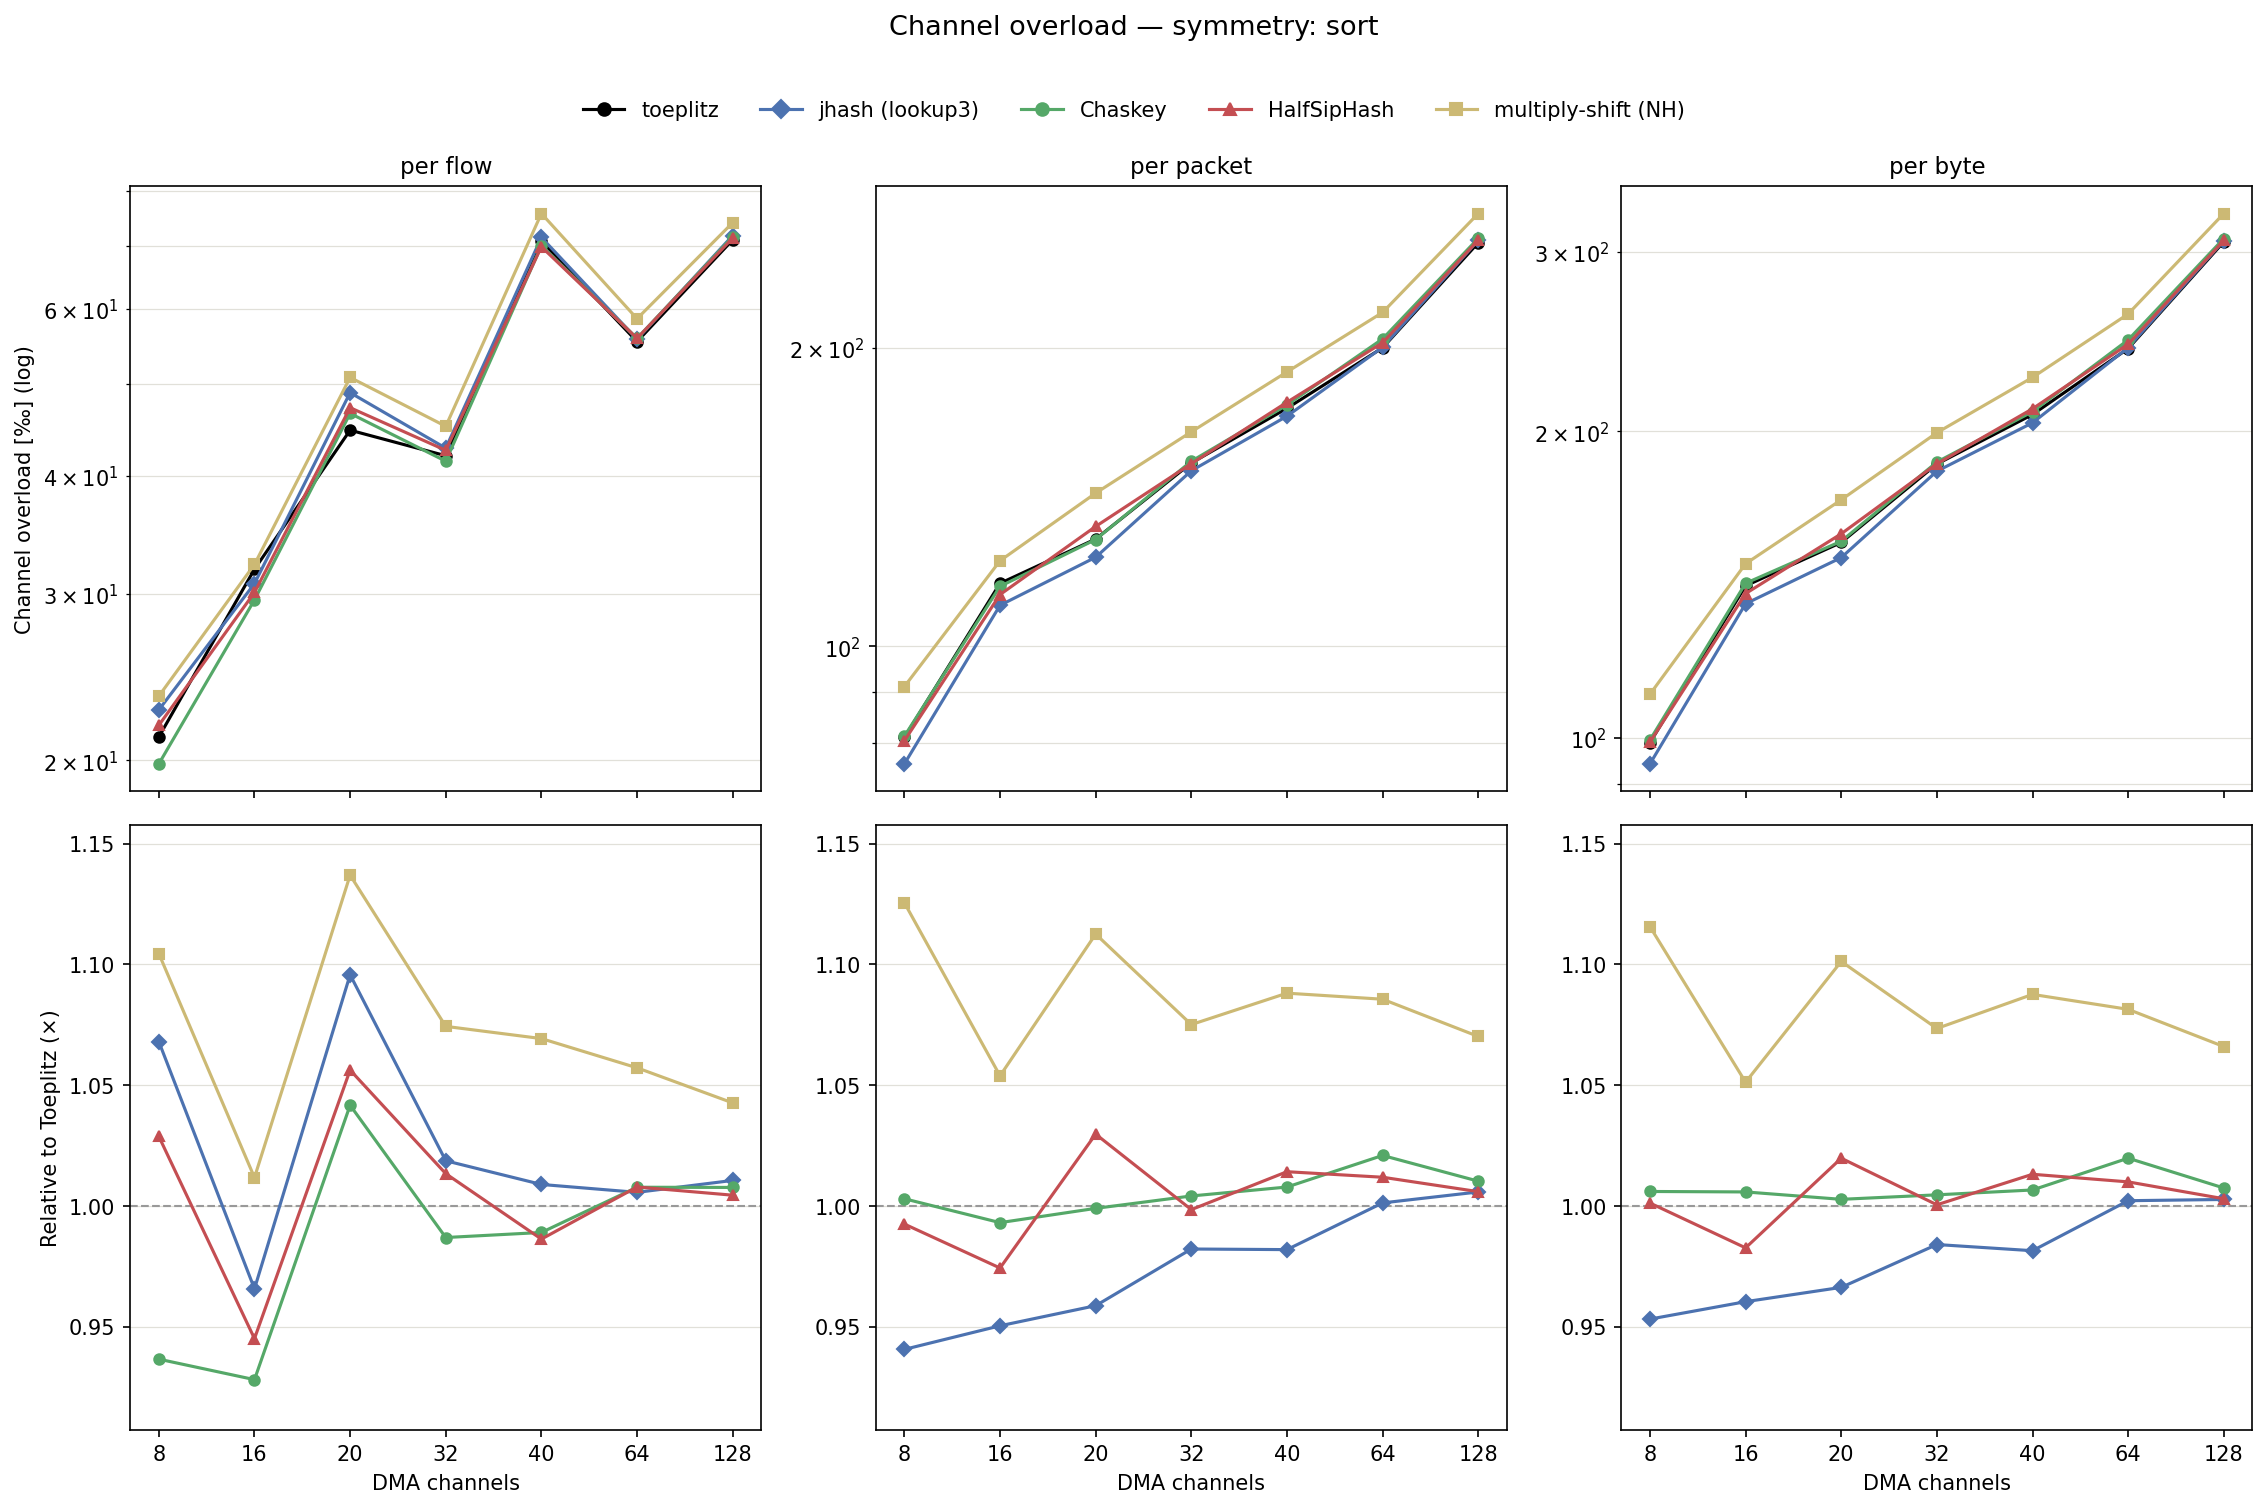
\includegraphics[width=\textwidth]{ostatne_vzorky/odid1_ip_only/overload_sortfold.png}
    \caption{symetria sort}
  \end{subfigure}

  \caption{Preťaženie funkcií a pomer k~Toeplitzu: \texttt{odid1}, iba IP adresy.}
  \label{fig:b-odid1-ip-only-overload}
\end{figure}

\begin{figure}[p]
  \centering
  \begin{subfigure}{0.54\textwidth}
    \centering
    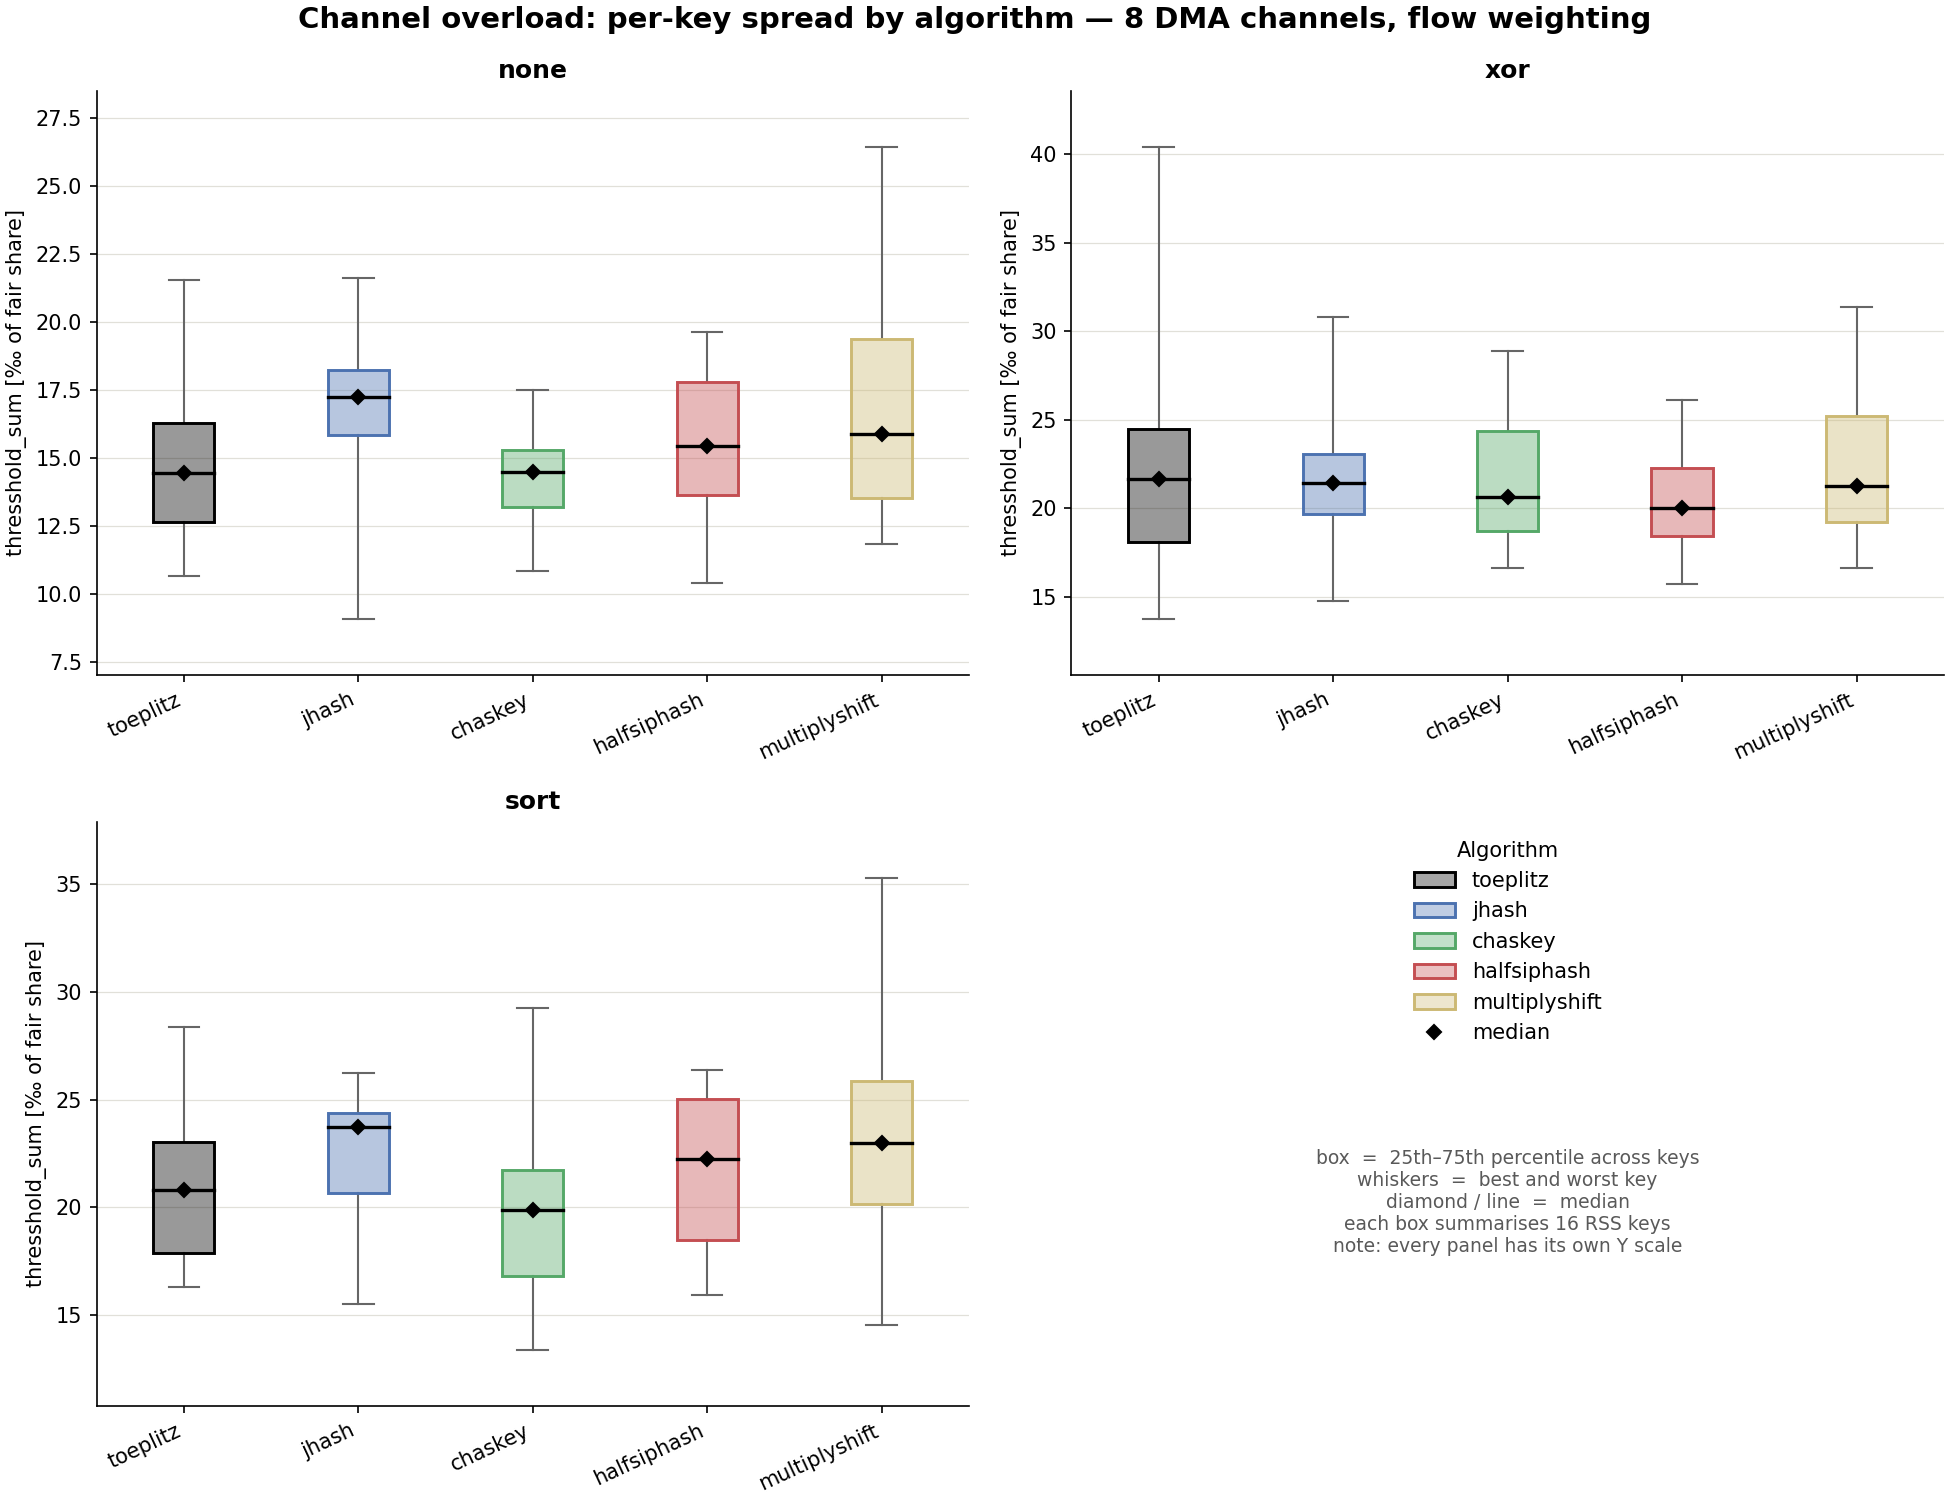
\includegraphics[width=\textwidth]{ostatne_vzorky/odid1_ip_only/keys_8.png}
    \caption{8 kanálov}
  \end{subfigure}

  \begin{subfigure}{0.54\textwidth}
    \centering
    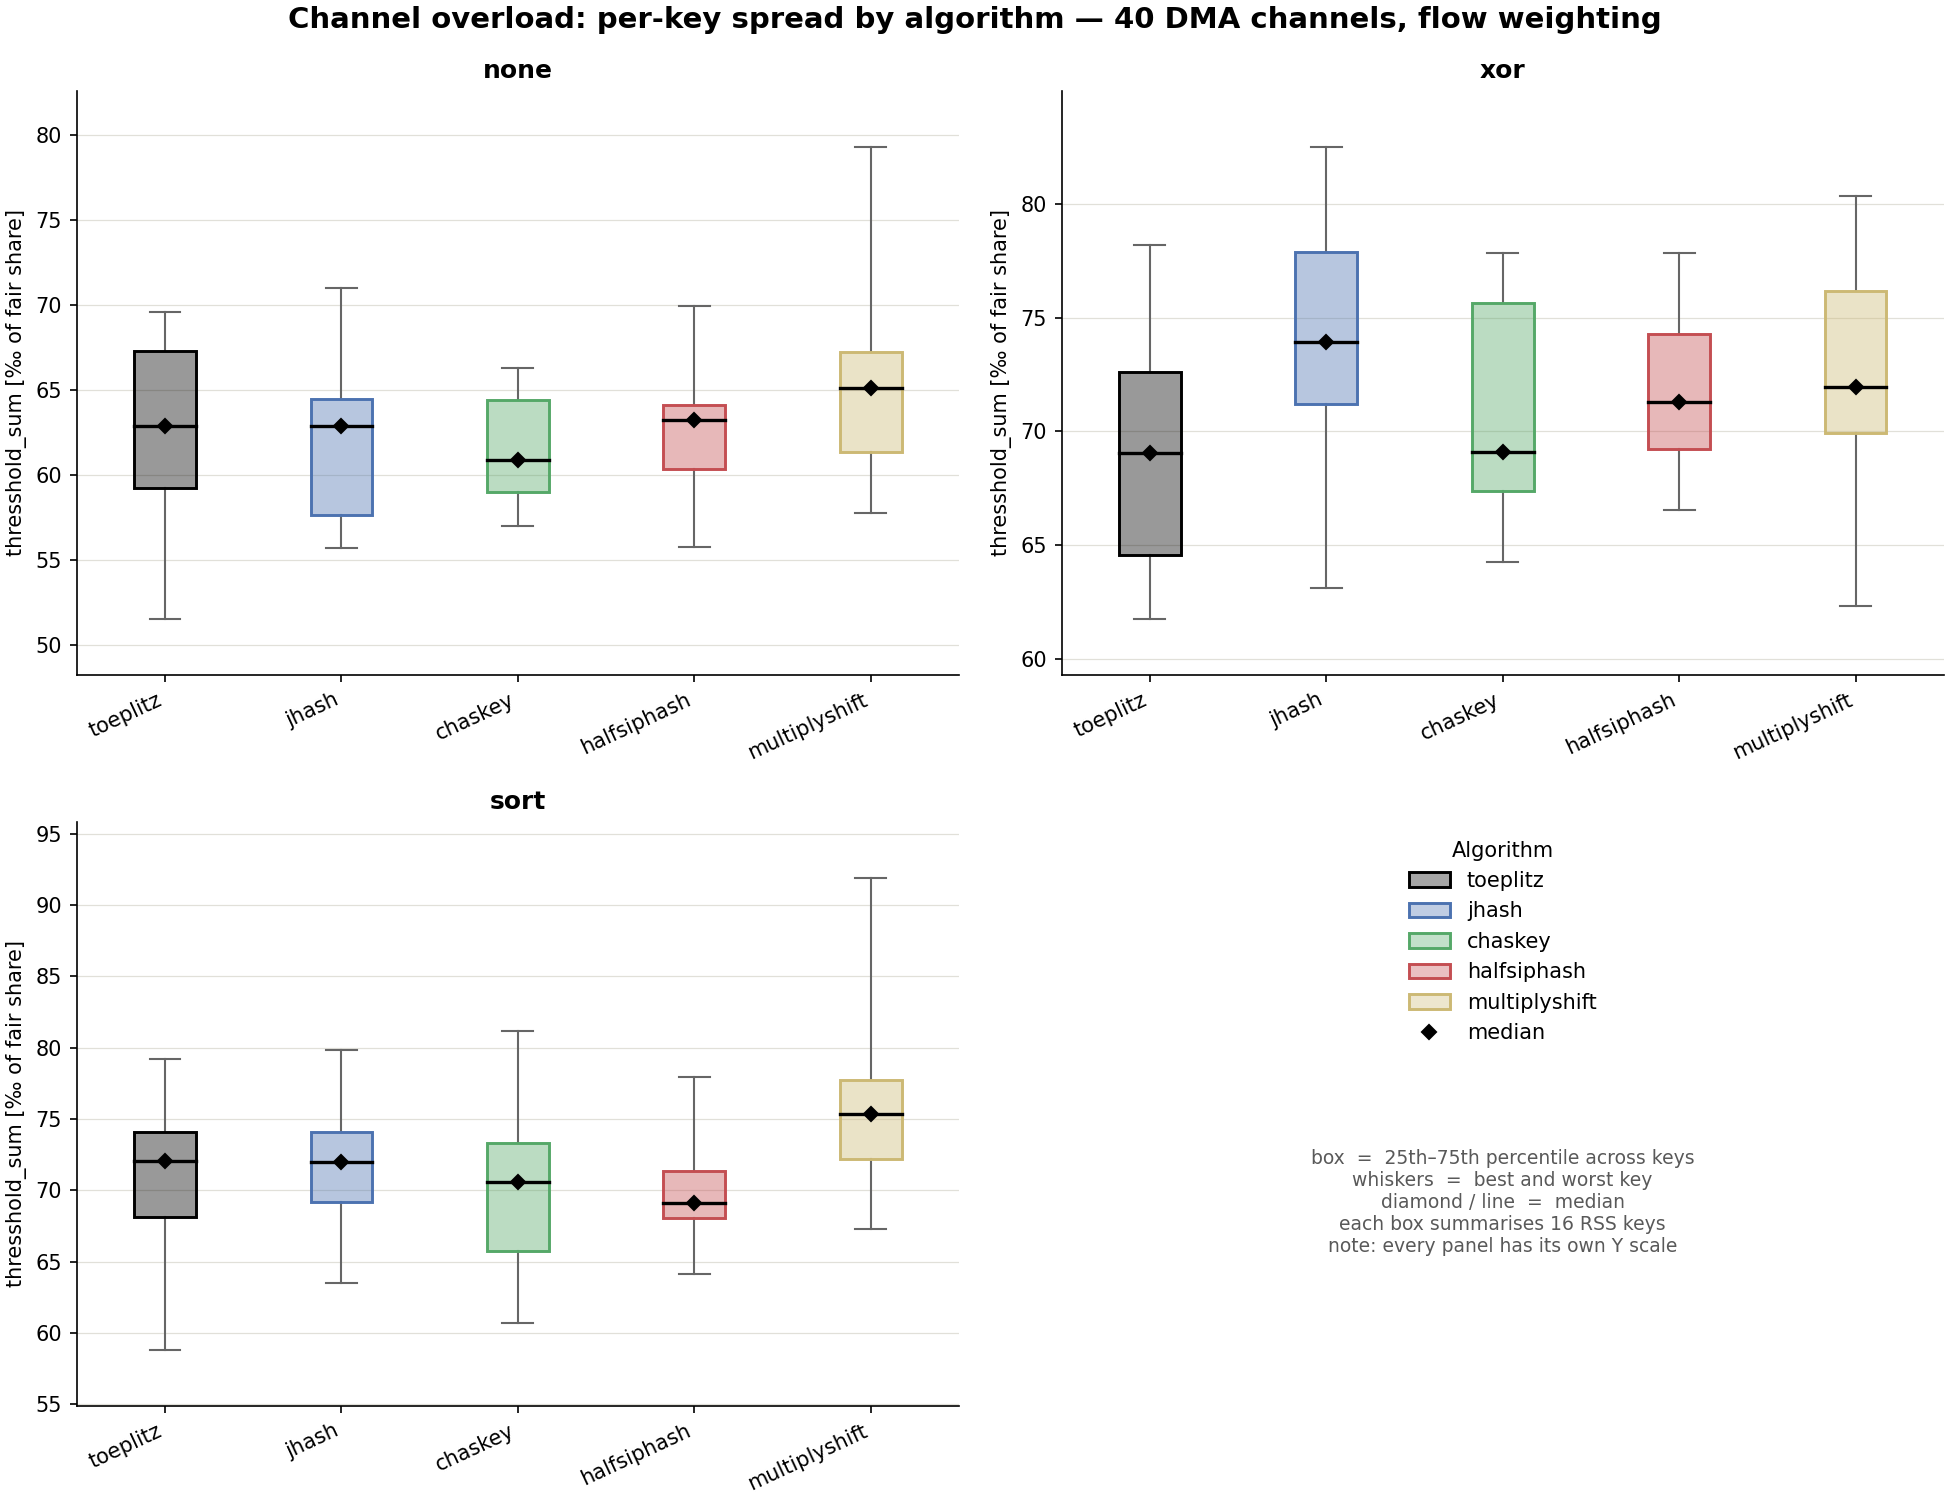
\includegraphics[width=\textwidth]{ostatne_vzorky/odid1_ip_only/keys_40.png}
    \caption{40 kanálov}
  \end{subfigure}

  \begin{subfigure}{0.54\textwidth}
    \centering
    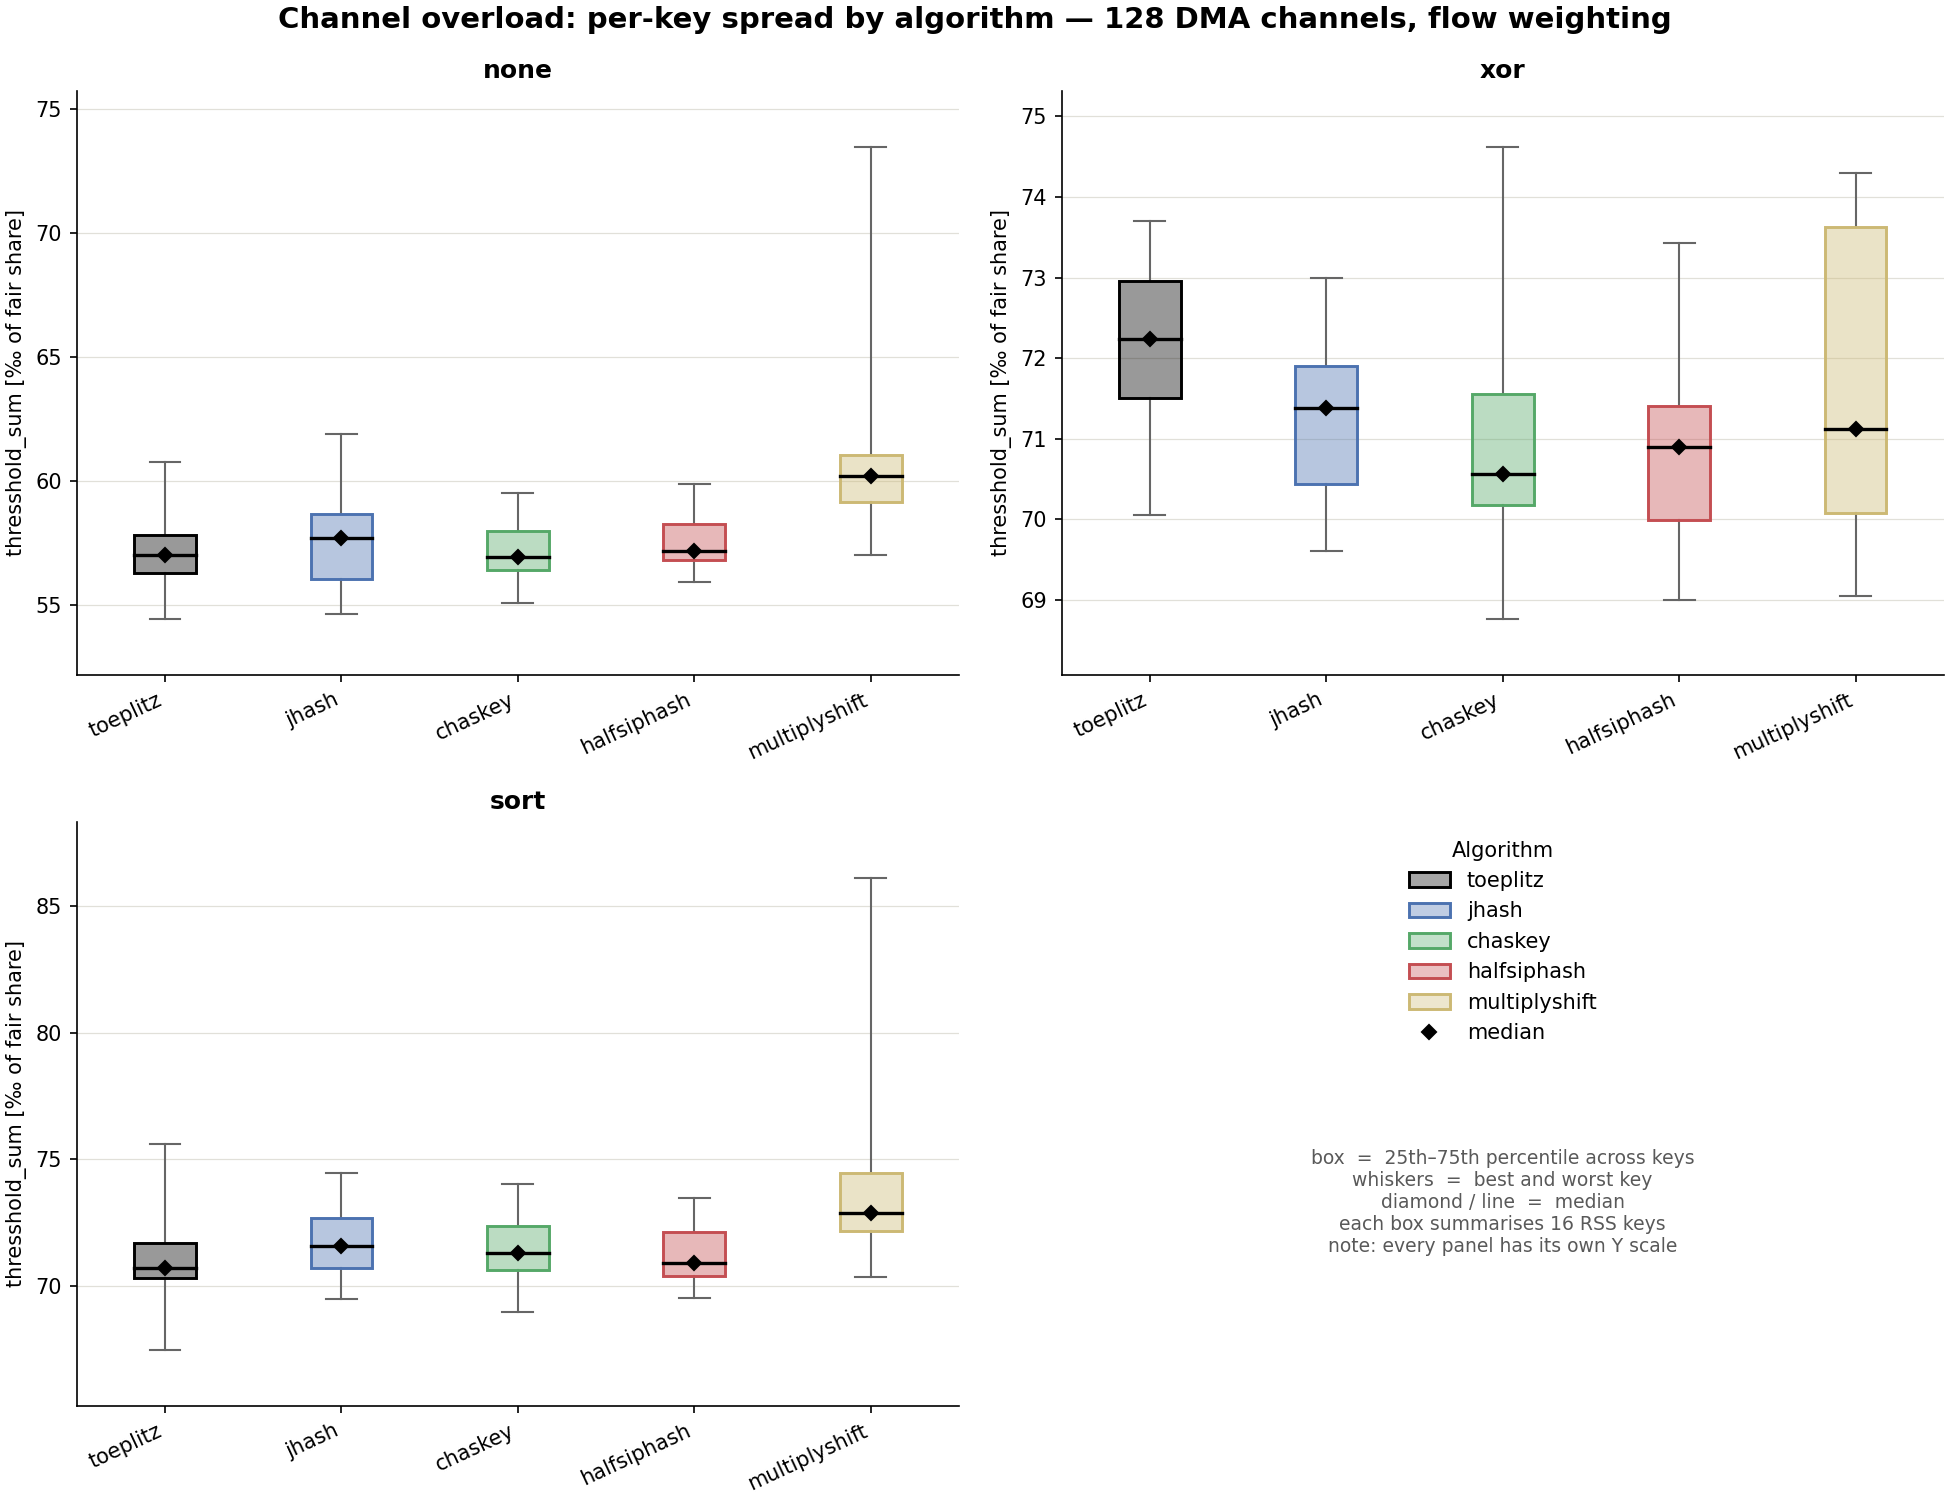
\includegraphics[width=\textwidth]{ostatne_vzorky/odid1_ip_only/keys_128.png}
    \caption{128 kanálov}
  \end{subfigure}

  \caption{Rozptyl preťaženia medzi 16 kľúčmi pri váhe \texttt{flow}: \texttt{odid1}, iba IP adresy.}
  \label{fig:b-odid1-ip-only-keys}
\end{figure}

\begin{figure}[ht]
  \centering
  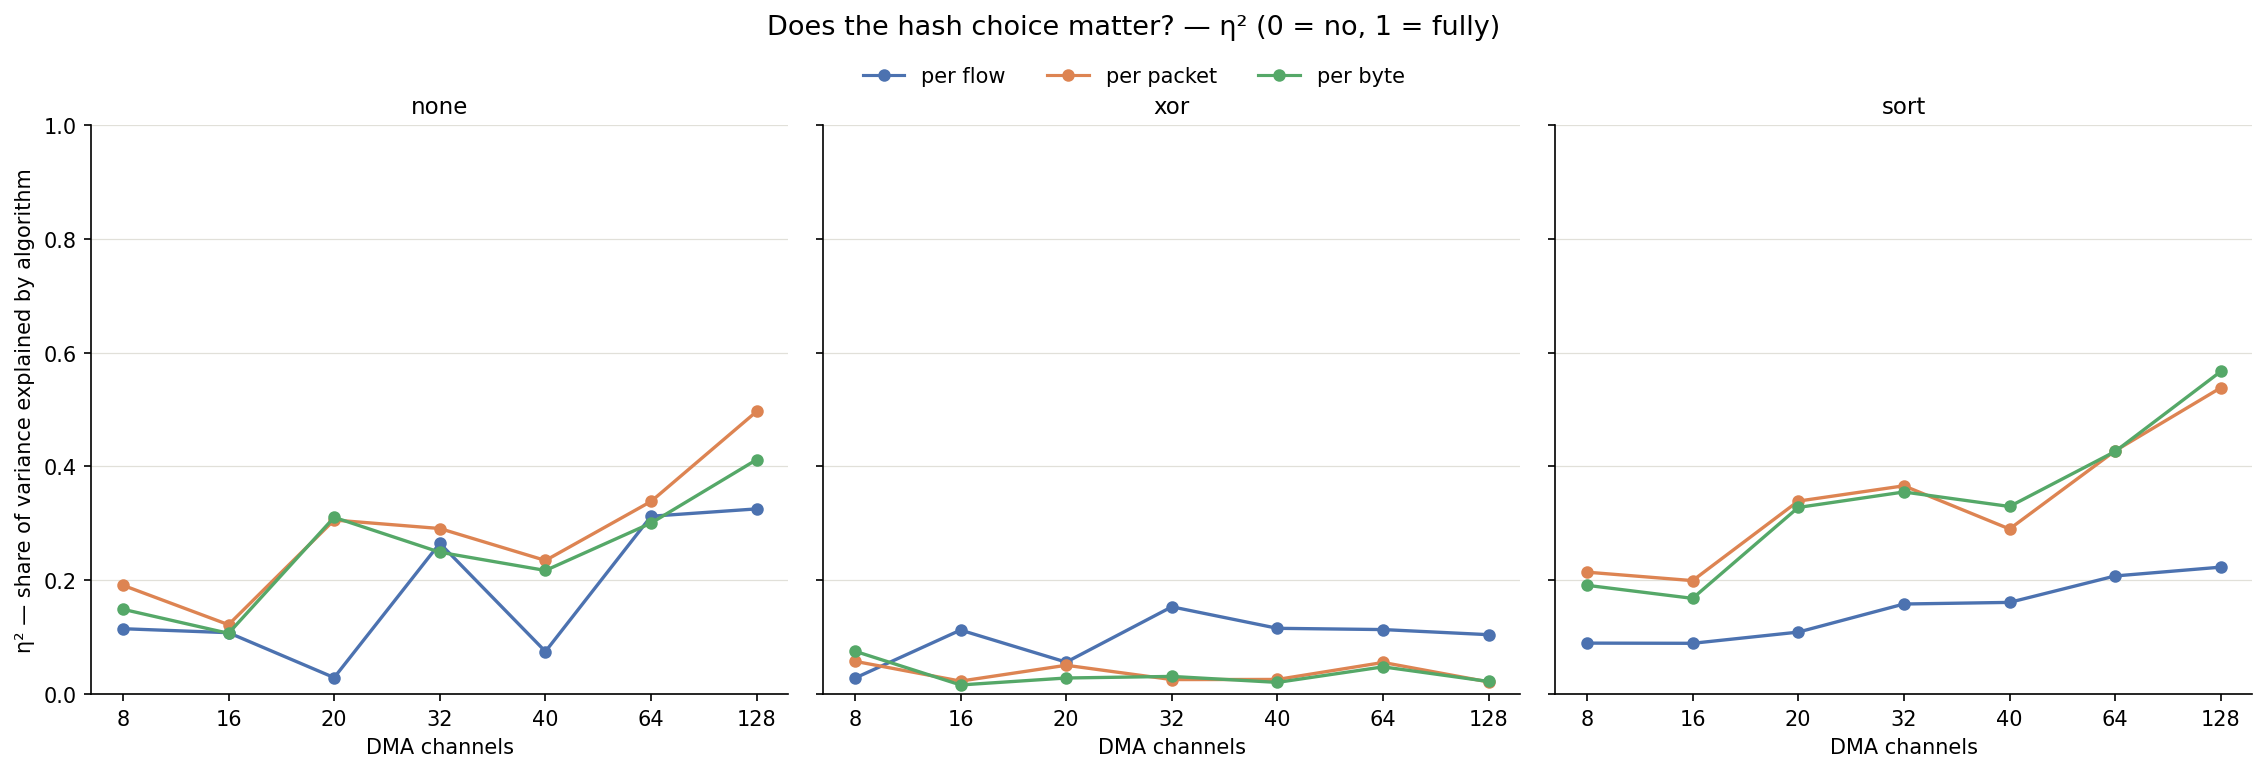
\includegraphics[width=0.9\textwidth]{ostatne_vzorky/odid1_ip_only/spread.png}
  \caption{Podiel rozptylu vysvetlený voľbou funkcie ($\eta^2$): \texttt{odid1}, iba IP adresy.}
  \label{fig:b-odid1-ip-only-spread}
\end{figure}
